% 数据图插入清单（20 张 DATA 图，由 figures/gen_fig_*.py 生成）
% 输出格式 docx：图为 PNG；width 取各脚本 set_paper_placement 声明的版面占比。
% 用法：把需要的 figure 环境复制到正文对应小节，不要整文件 \input。

% ── 数据与物性 ────────────────────────────────────────────────
\begin{figure}[H]
  \centering
  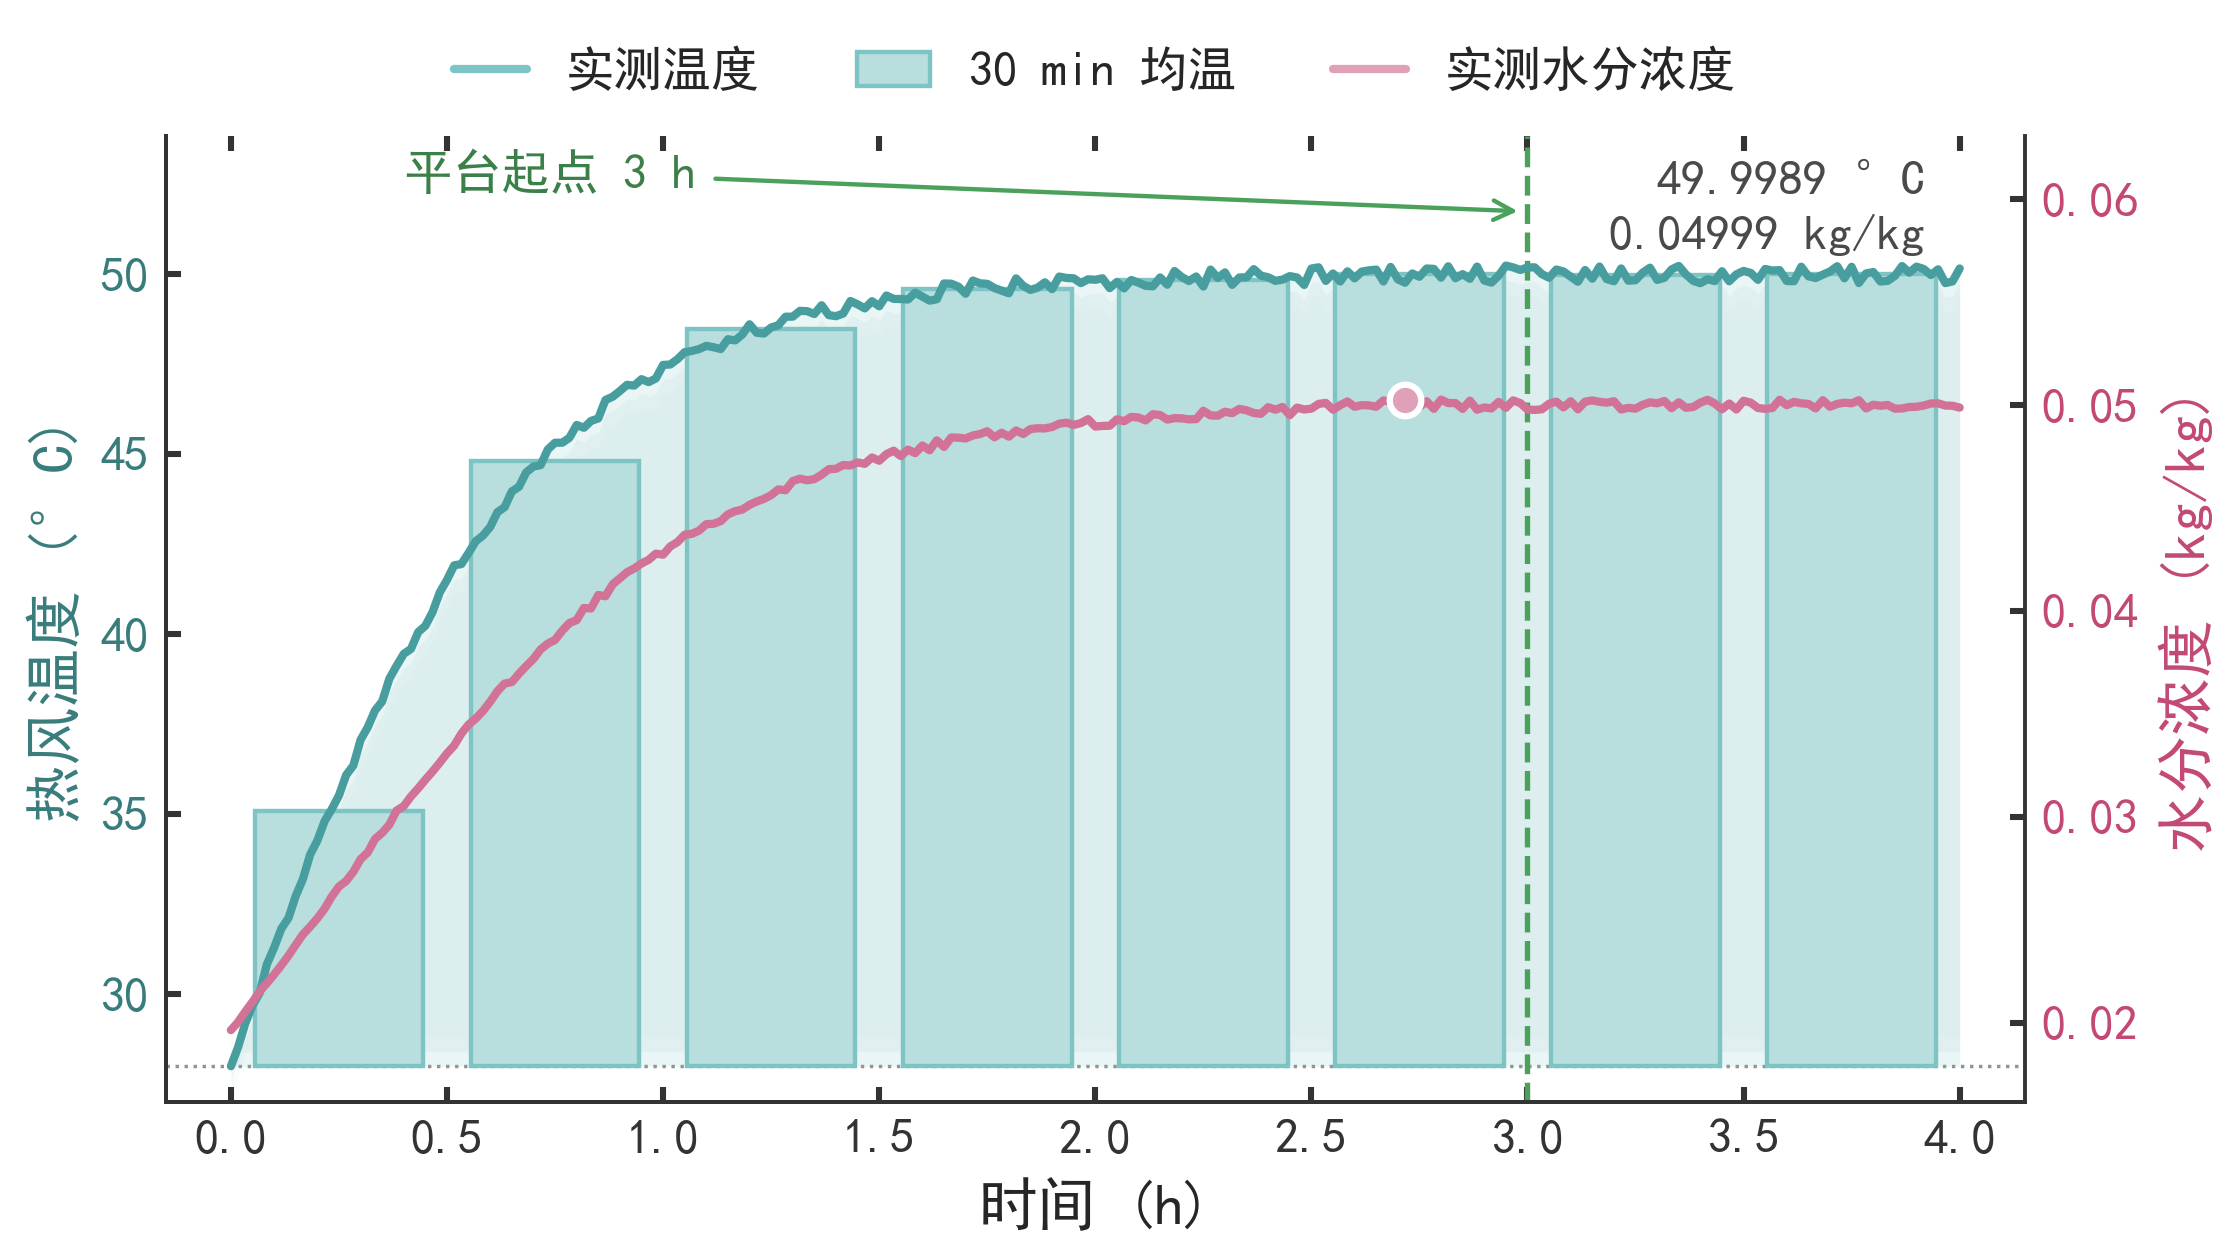
\includegraphics[width=0.90\textwidth]{figures/fig_oven_input.png}
  \caption{烘房温度与水分浓度演化}
  \label{fig:oven_input}
\end{figure}

\begin{figure}[H]
  \centering
  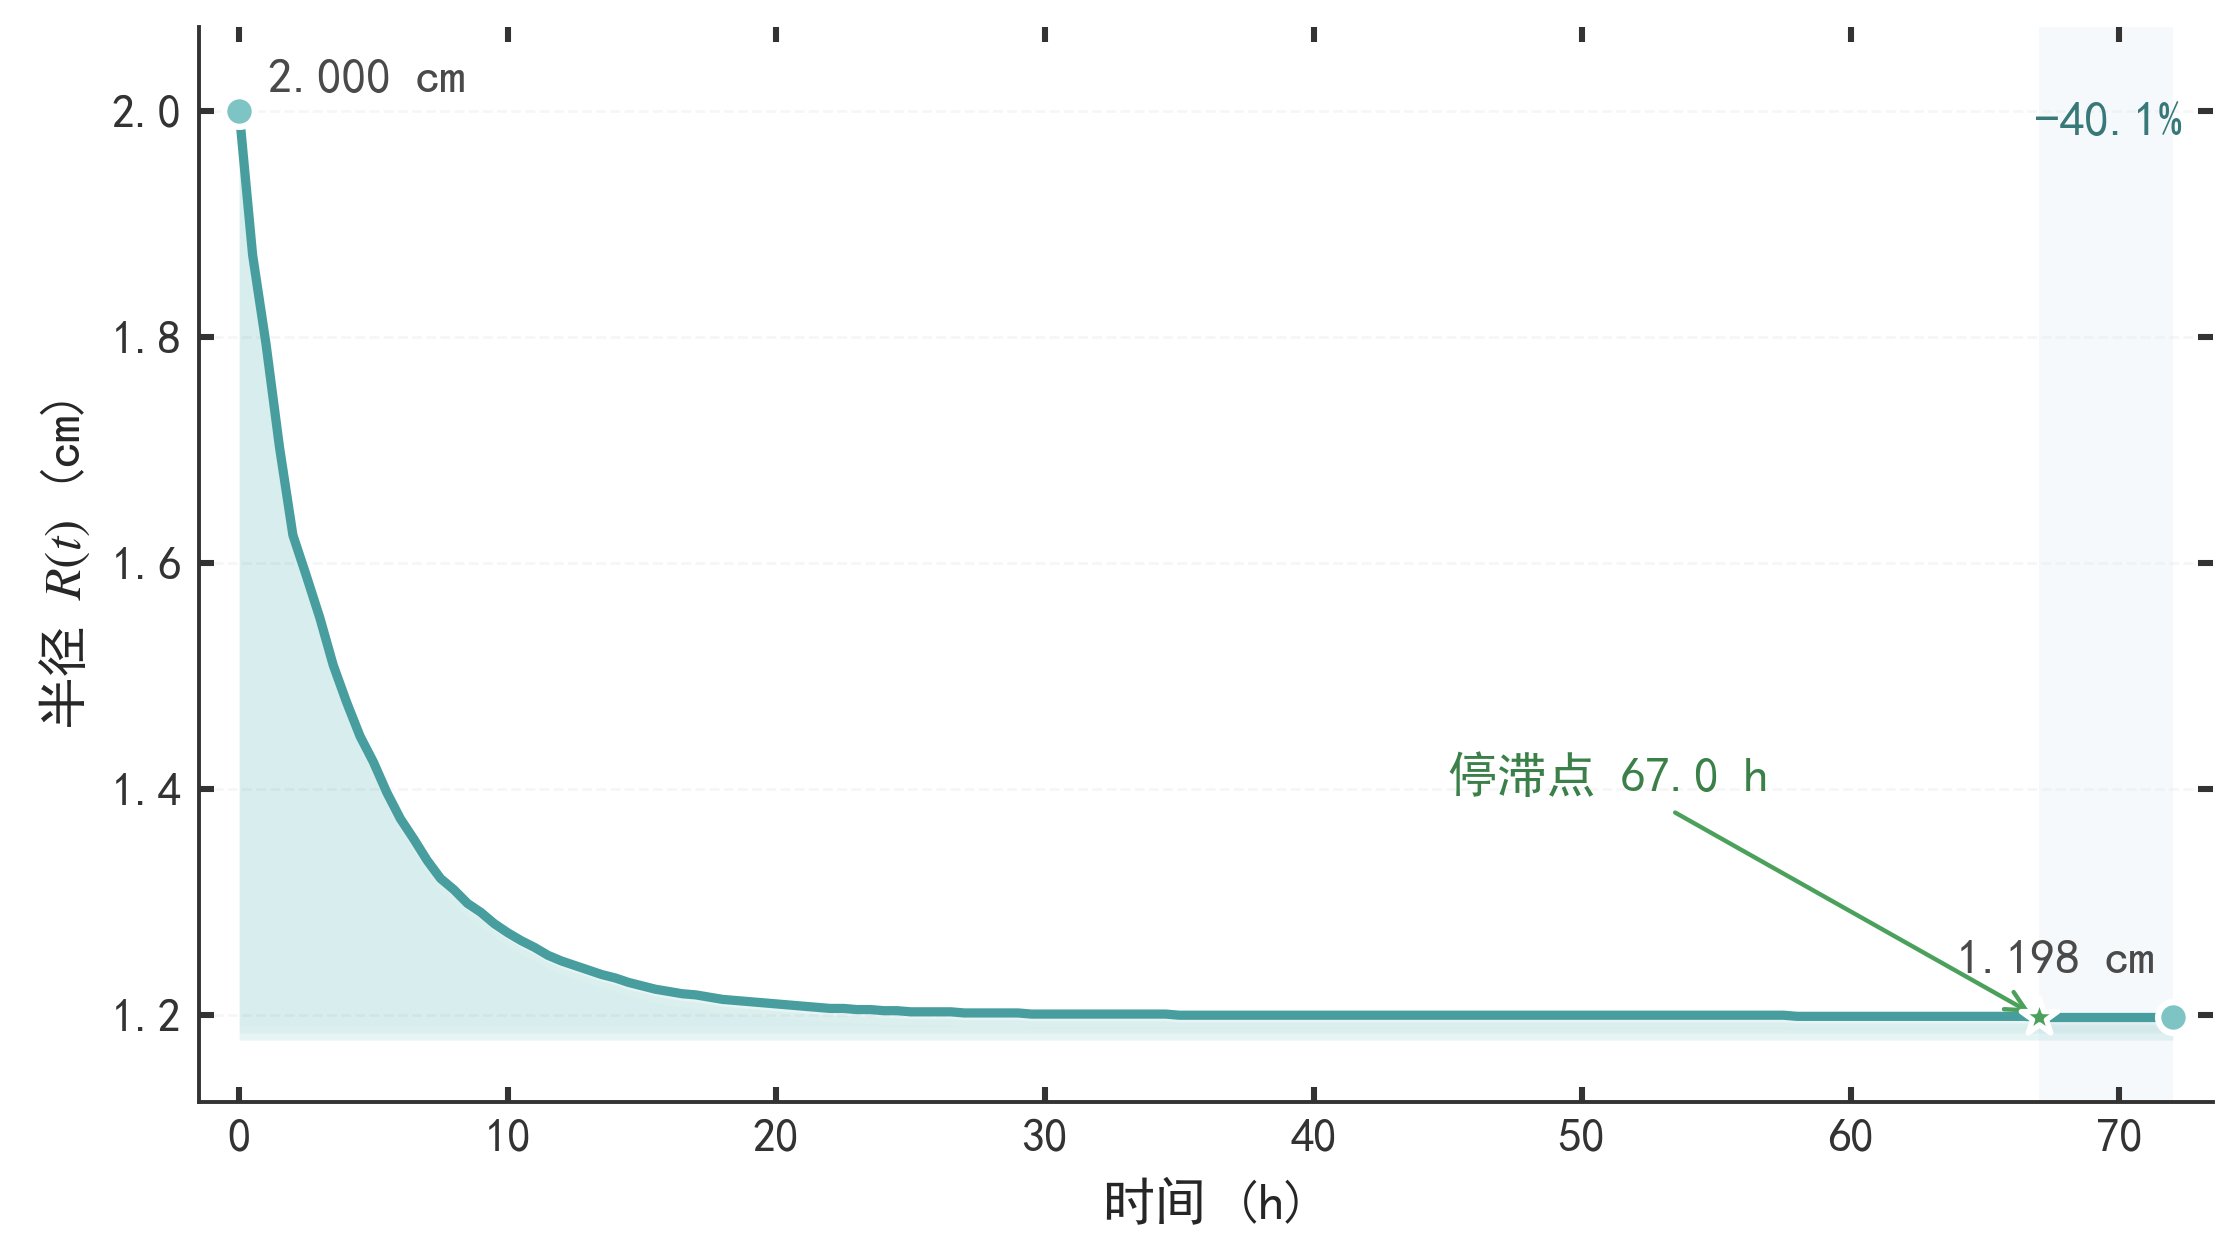
\includegraphics[width=0.90\textwidth]{figures/fig_shrink_radius.png}
  \caption{药材半径收缩曲线}
  \label{fig:shrink_radius}
\end{figure}

\begin{figure}[H]
  \centering
  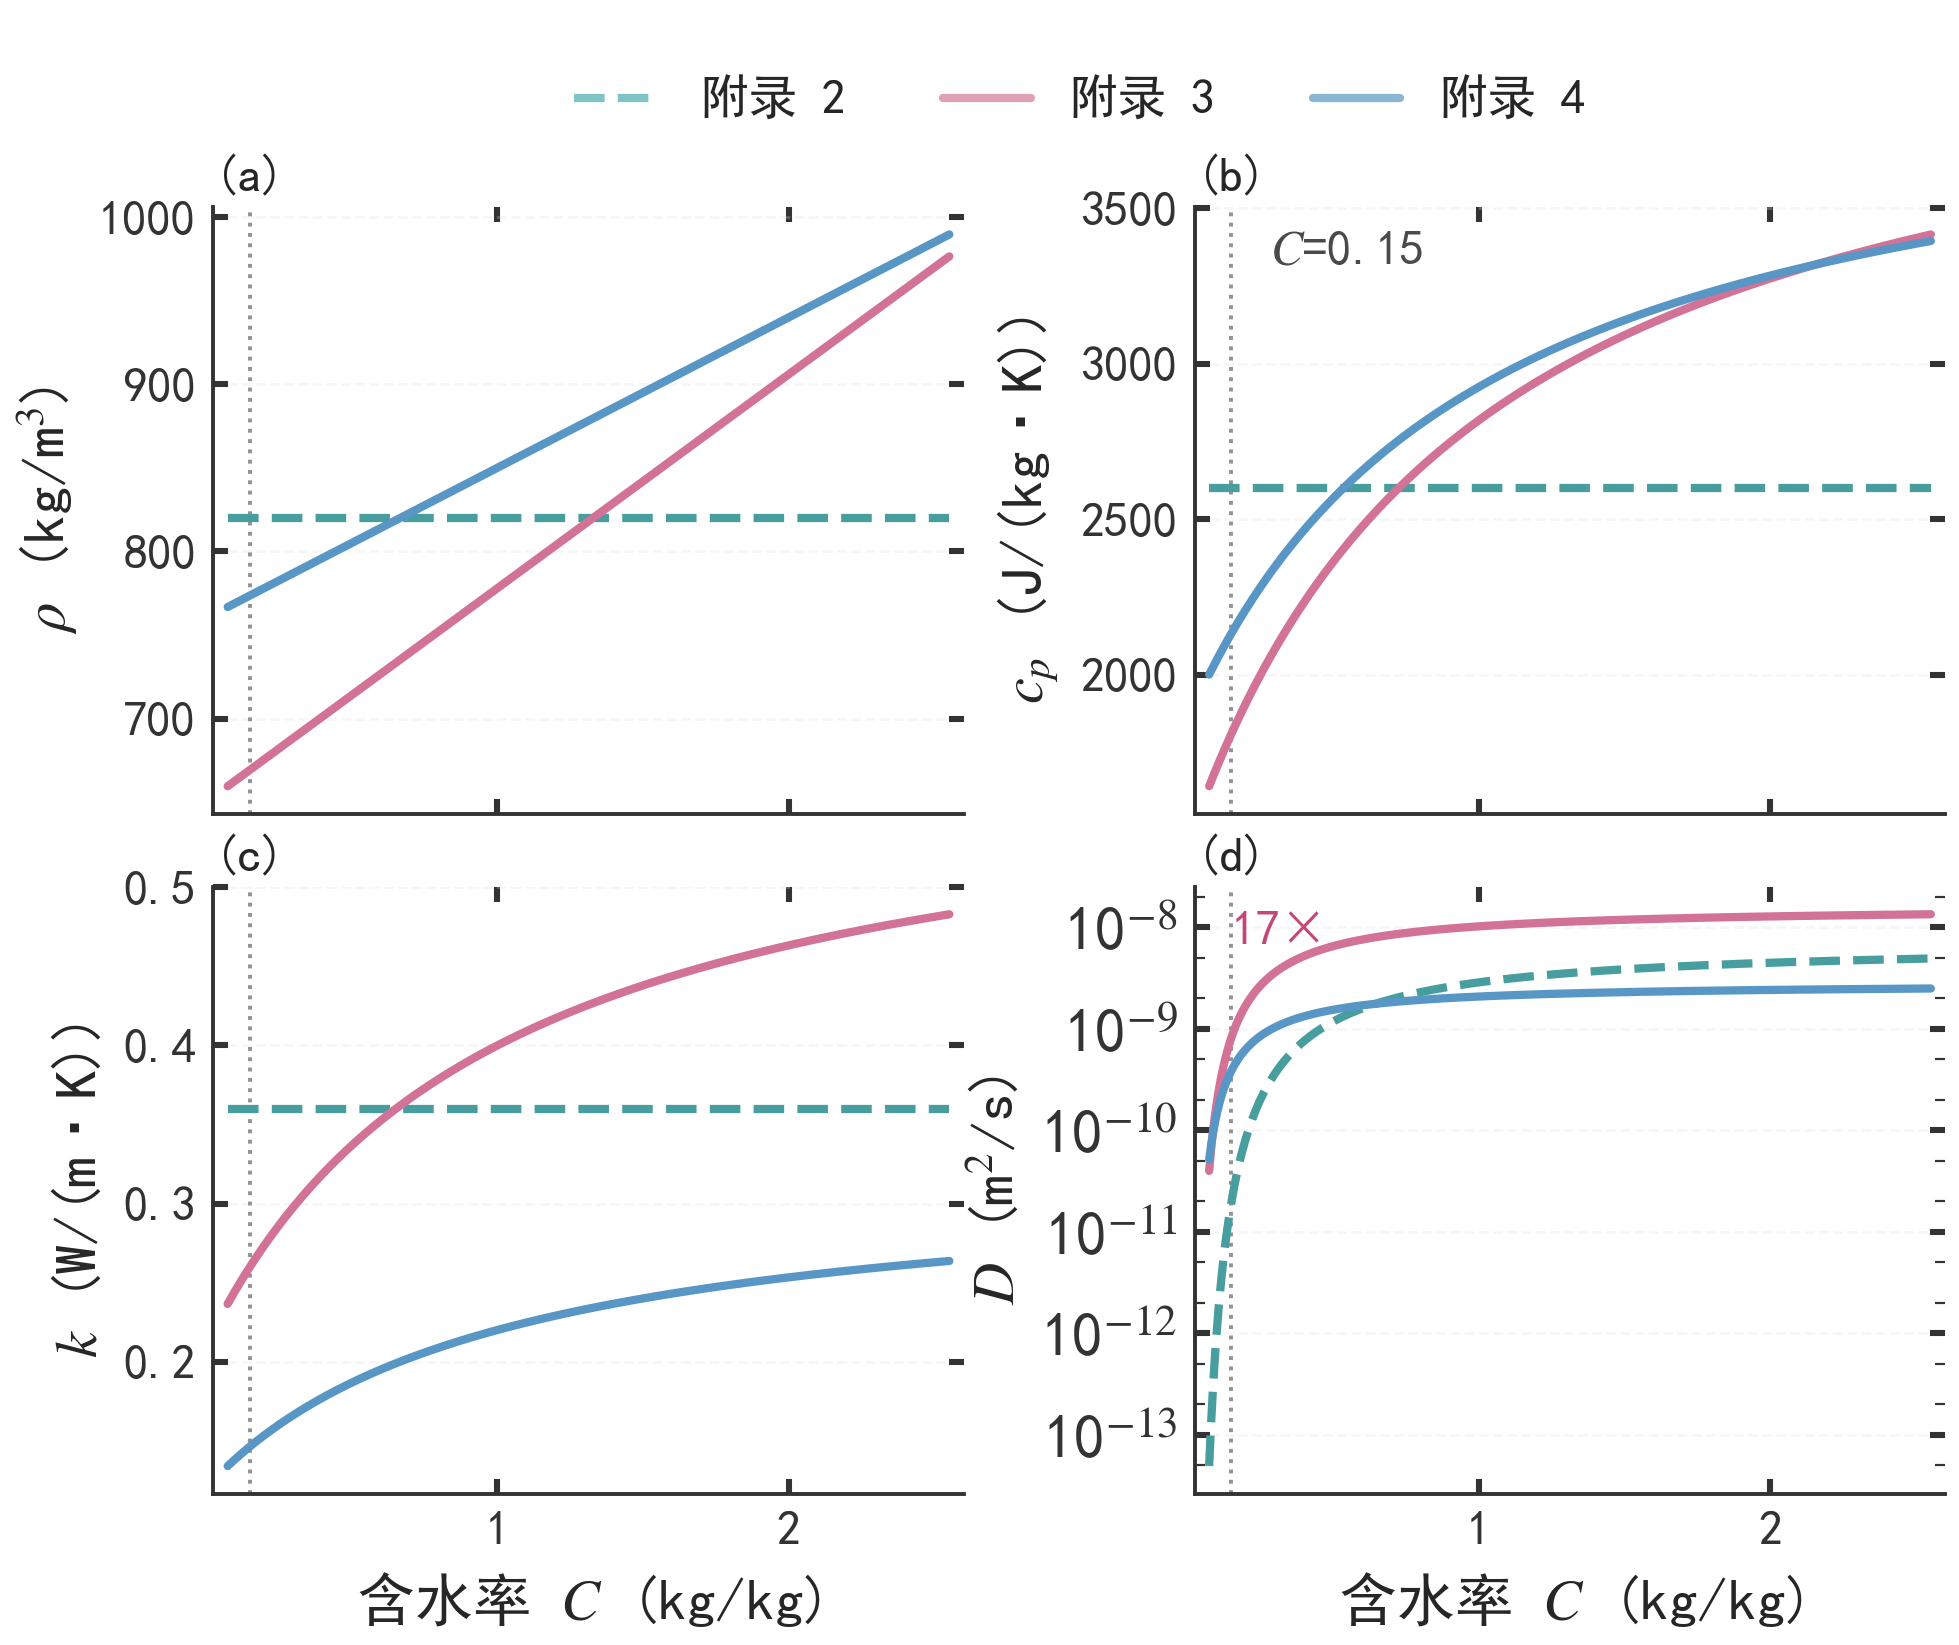
\includegraphics[width=0.80\textwidth]{figures/fig_property_laws.png}
  \caption{三组物性随含水率的变化}
  \label{fig:property_laws}
\end{figure}

\begin{figure}[H]
  \centering
  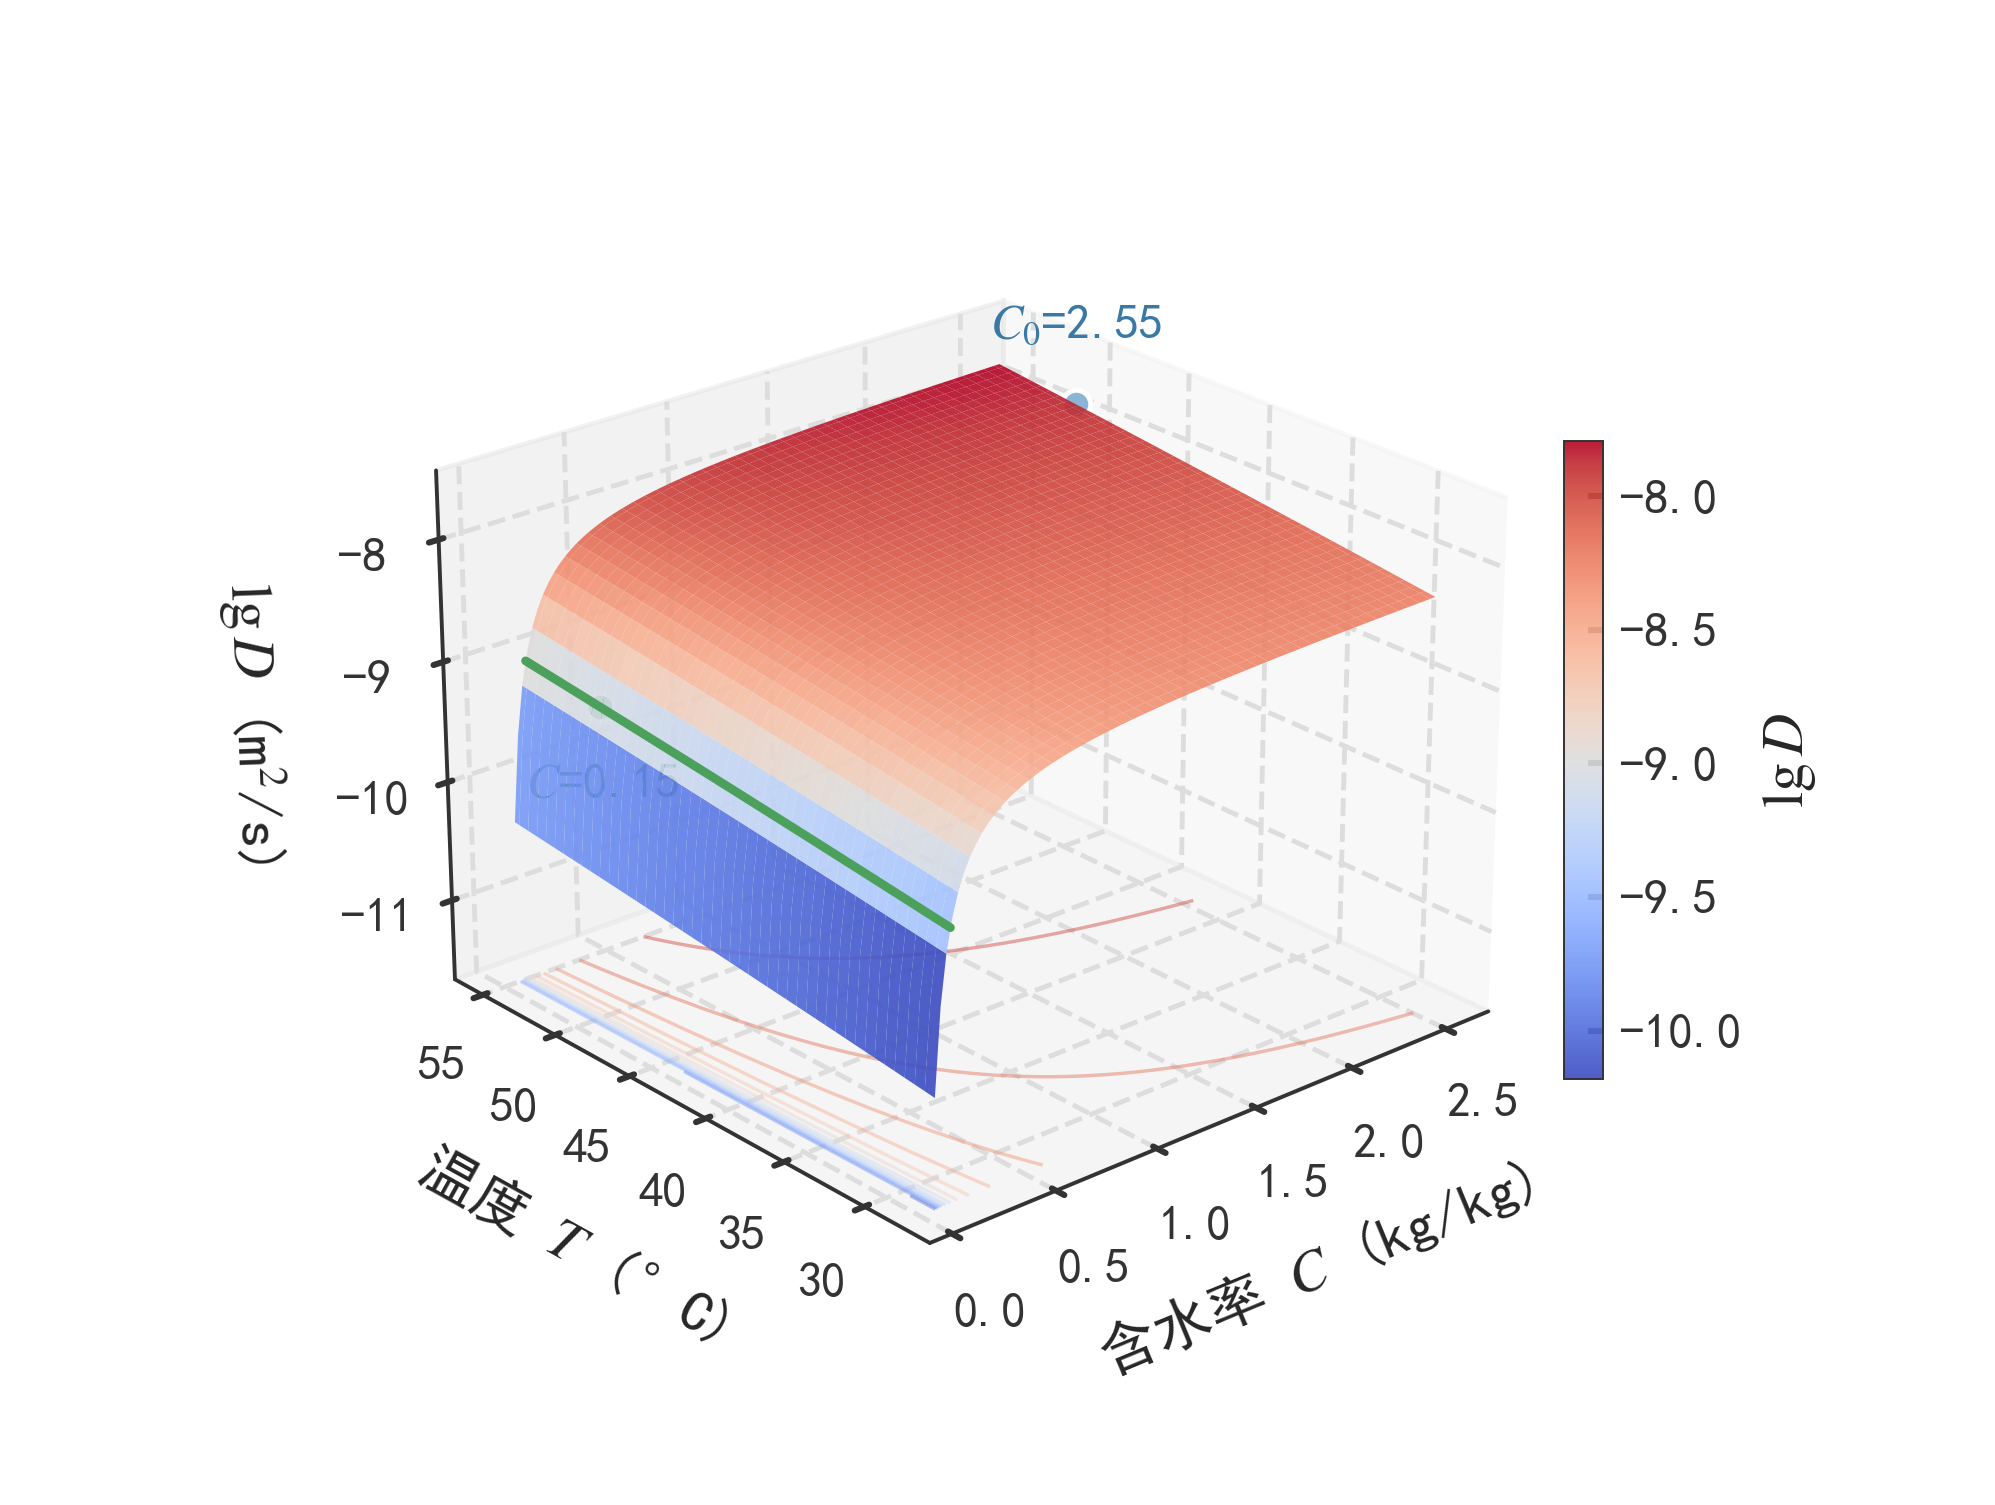
\includegraphics[width=0.80\textwidth]{figures/fig_D_landscape.png}
  \caption{扩散系数在 $(C,T)$ 平面的地形}
  \label{fig:D_landscape}
\end{figure}

% ── 问题 1 ────────────────────────────────────────────────────
\begin{figure}[H]
  \centering
  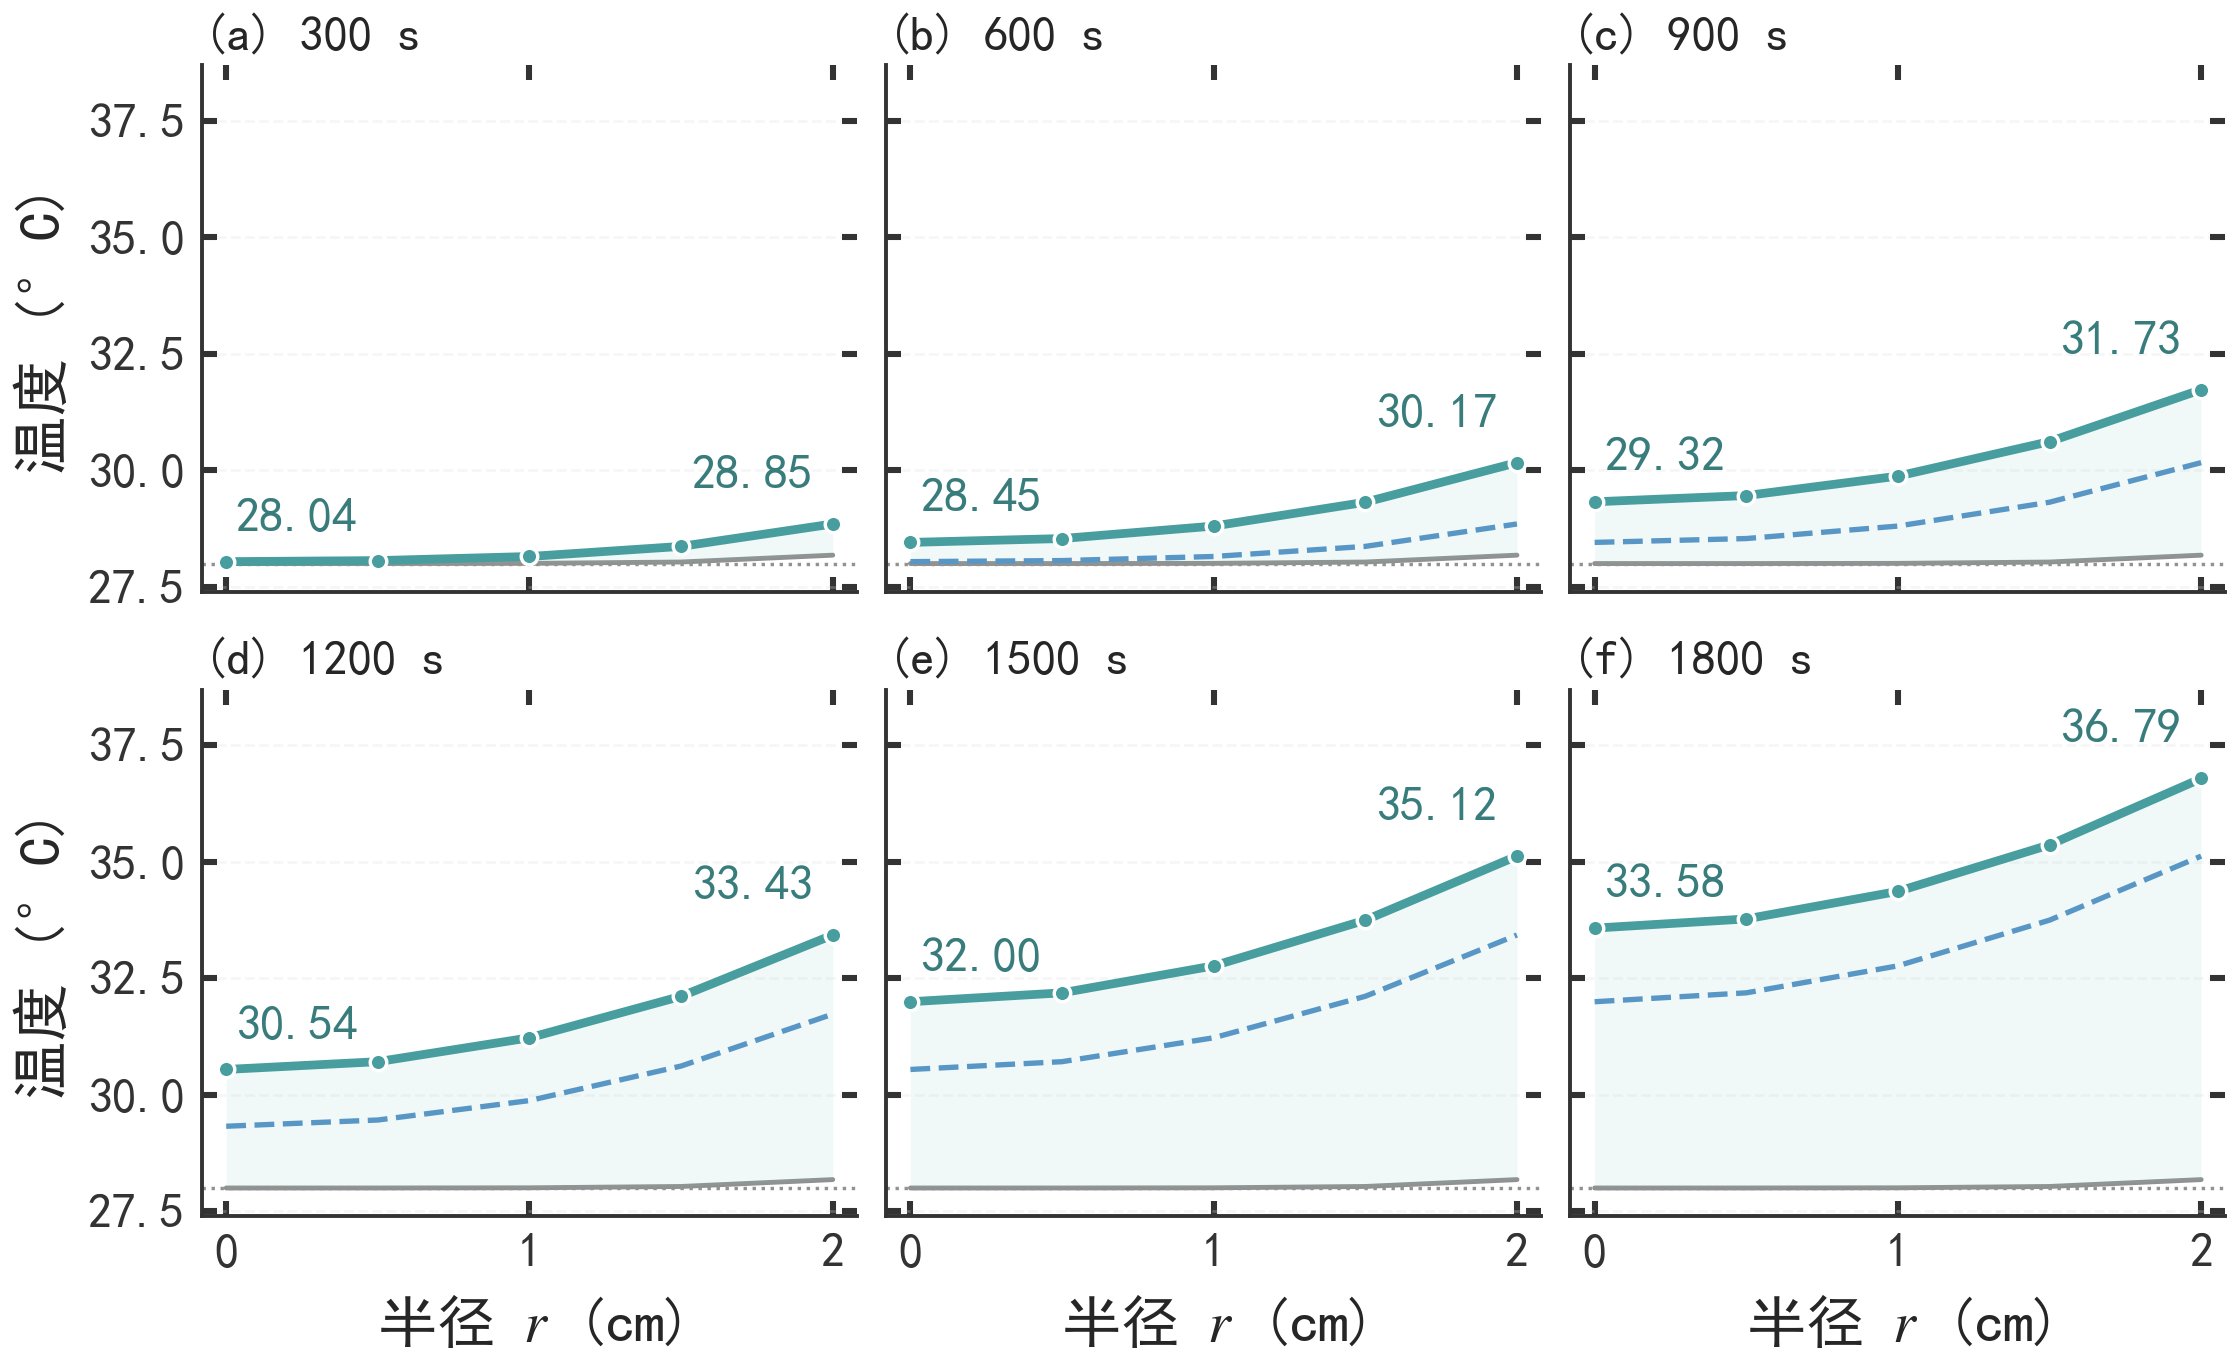
\includegraphics[width=0.90\textwidth]{figures/fig_q1_temp_profiles.png}
  \caption{预热段各时刻温度径向剖面}
  \label{fig:q1_temp_profiles}
\end{figure}

\begin{figure}[H]
  \centering
  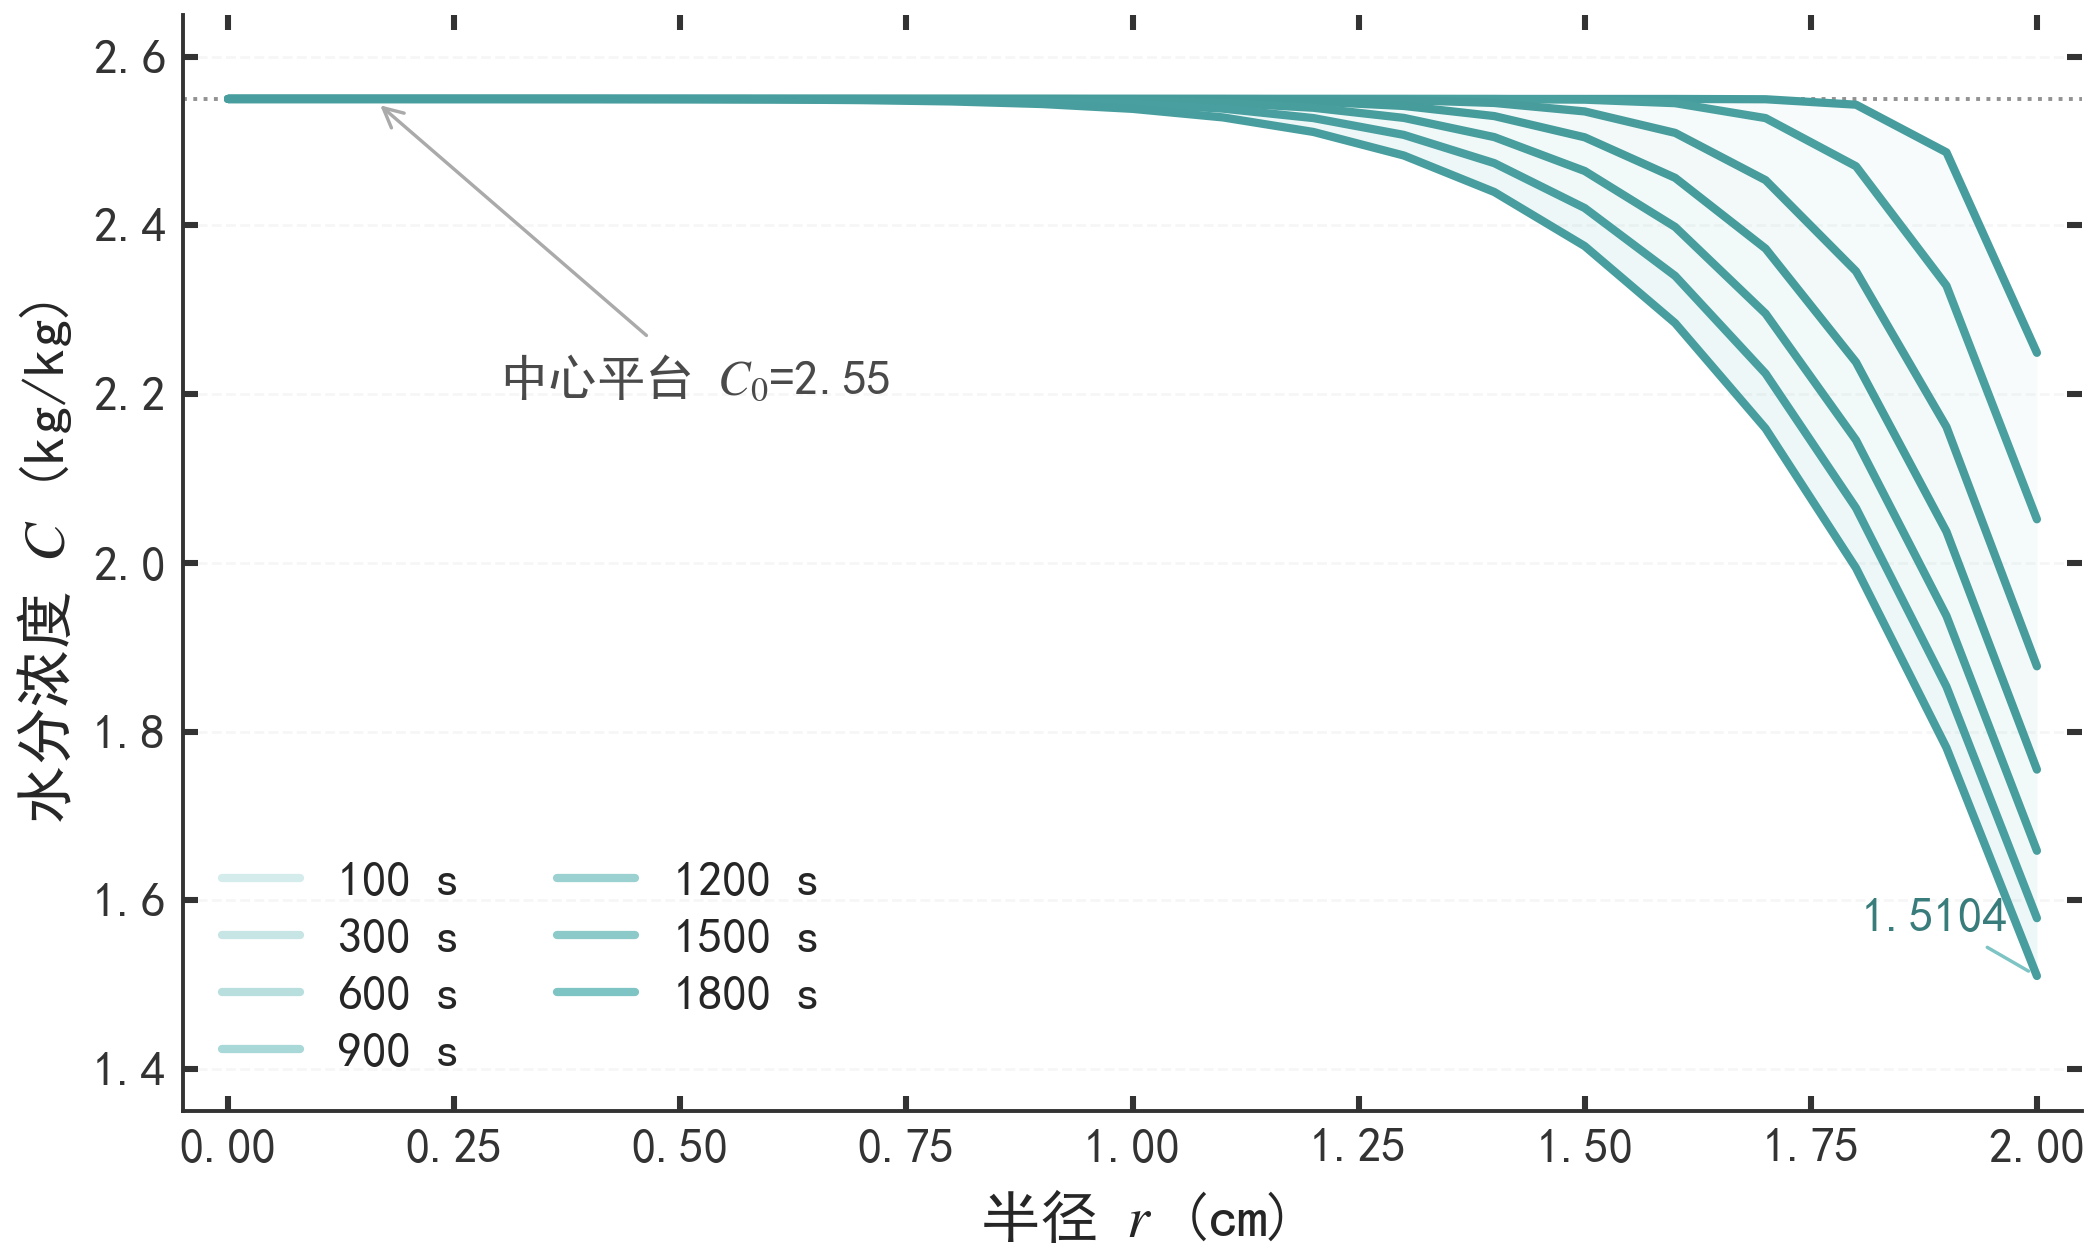
\includegraphics[width=0.86\textwidth]{figures/fig_q1_moist_profiles.png}
  \caption{预热段水分径向剖面}
  \label{fig:q1_moist_profiles}
\end{figure}

\begin{figure}[H]
  \centering
  
\includegraphics[width=0.86\textwidth]{figures/fig_q1_temp_field.png}
  \caption{预热段温度时空场}
  \label{fig:q1_temp_field}
\end{figure}

\begin{figure}[H]
  \centering
  
\includegraphics[width=0.86\textwidth]{figures/fig_q1_moist_field.png}
  \caption{预热段水分时空场与渗透前沿}
  \label{fig:q1_moist_field}
\end{figure}

\begin{figure}[H]
  \centering
  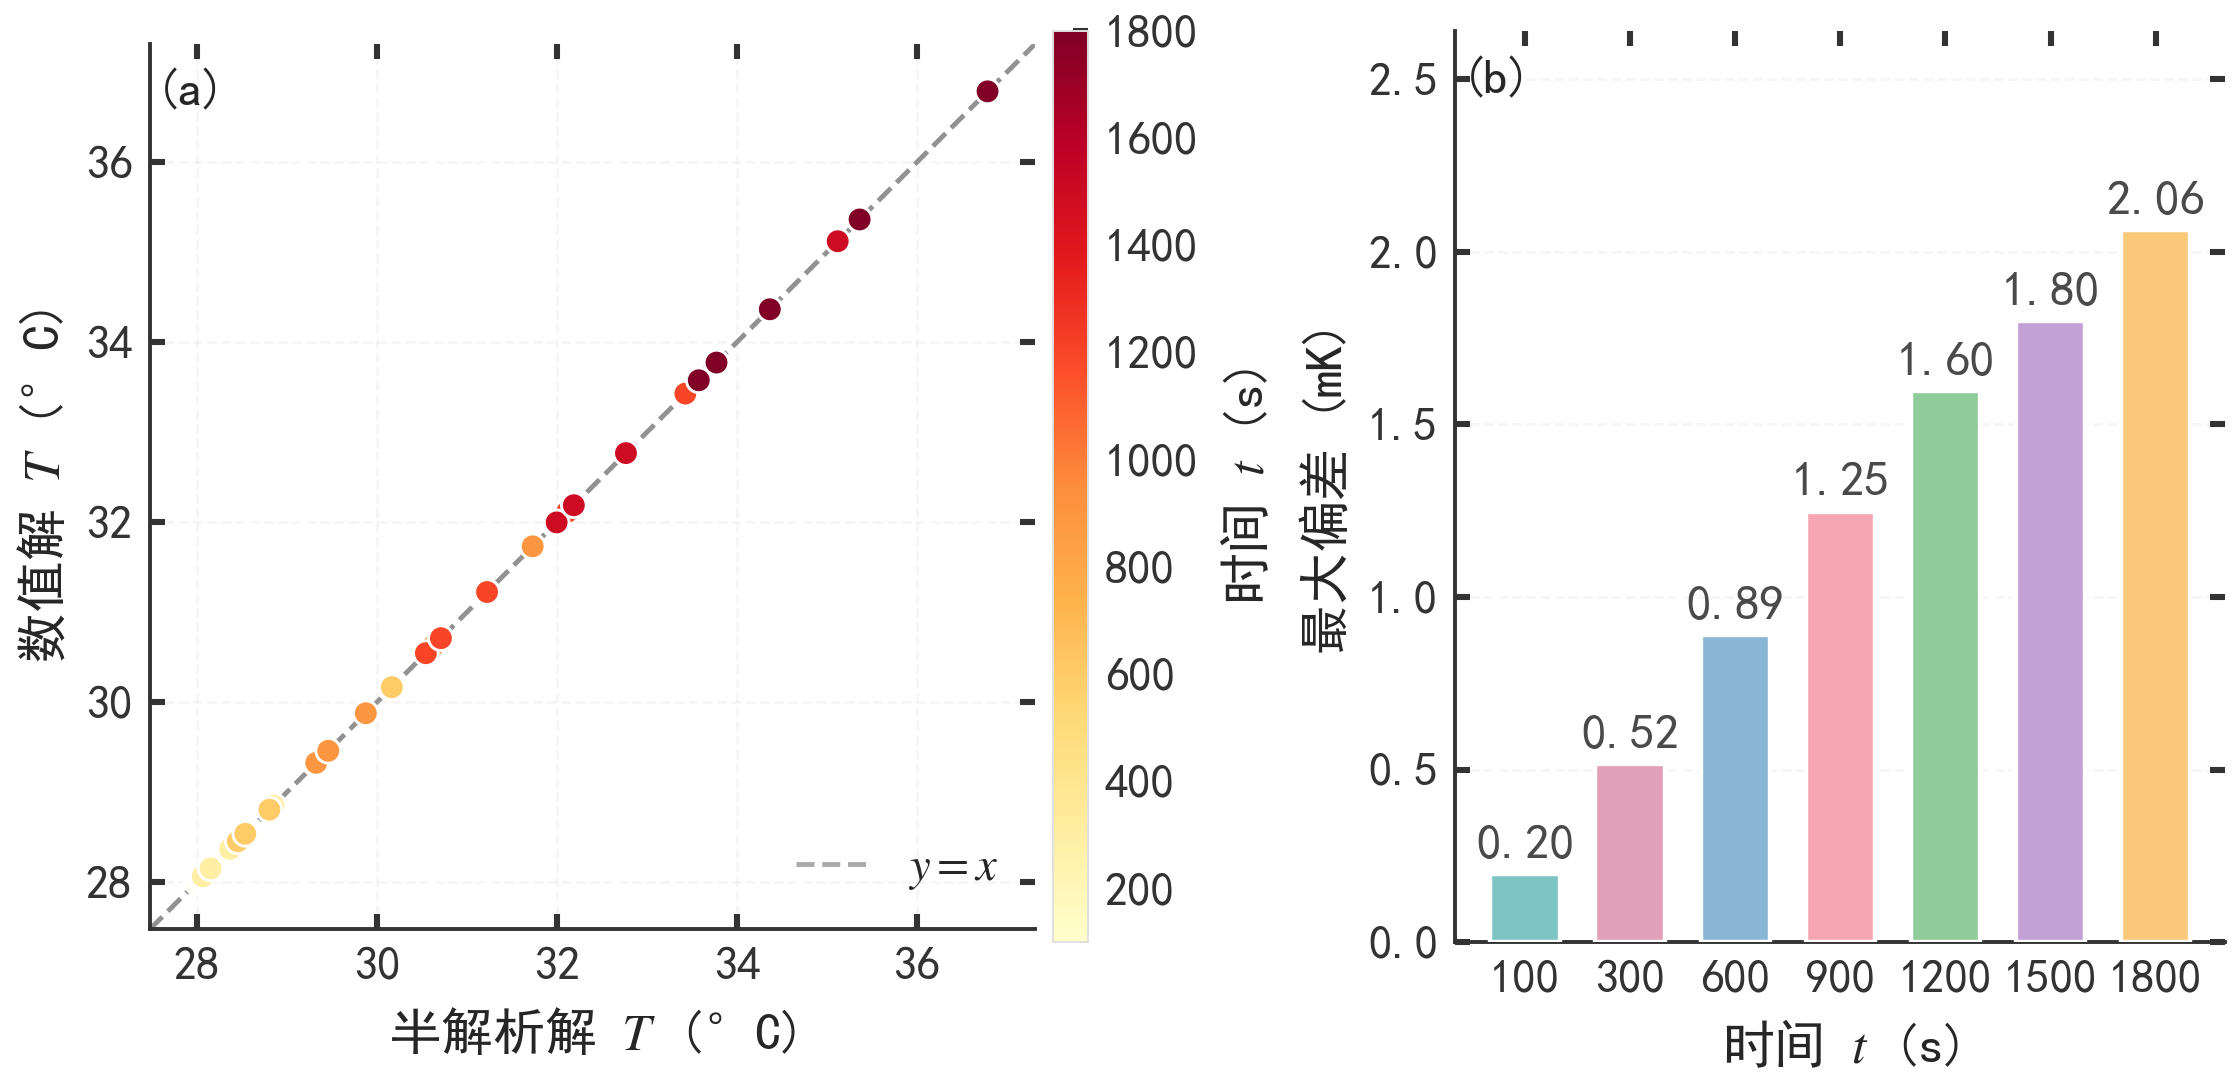
\includegraphics[width=0.94\textwidth]{figures/fig_q1_analytic_validation.png}
  \caption{数值解与级数解对照}
  \label{fig:q1_analytic_validation}
\end{figure}

% ── 问题 2 ────────────────────────────────────────────────────
\begin{figure}[H]
  \centering
  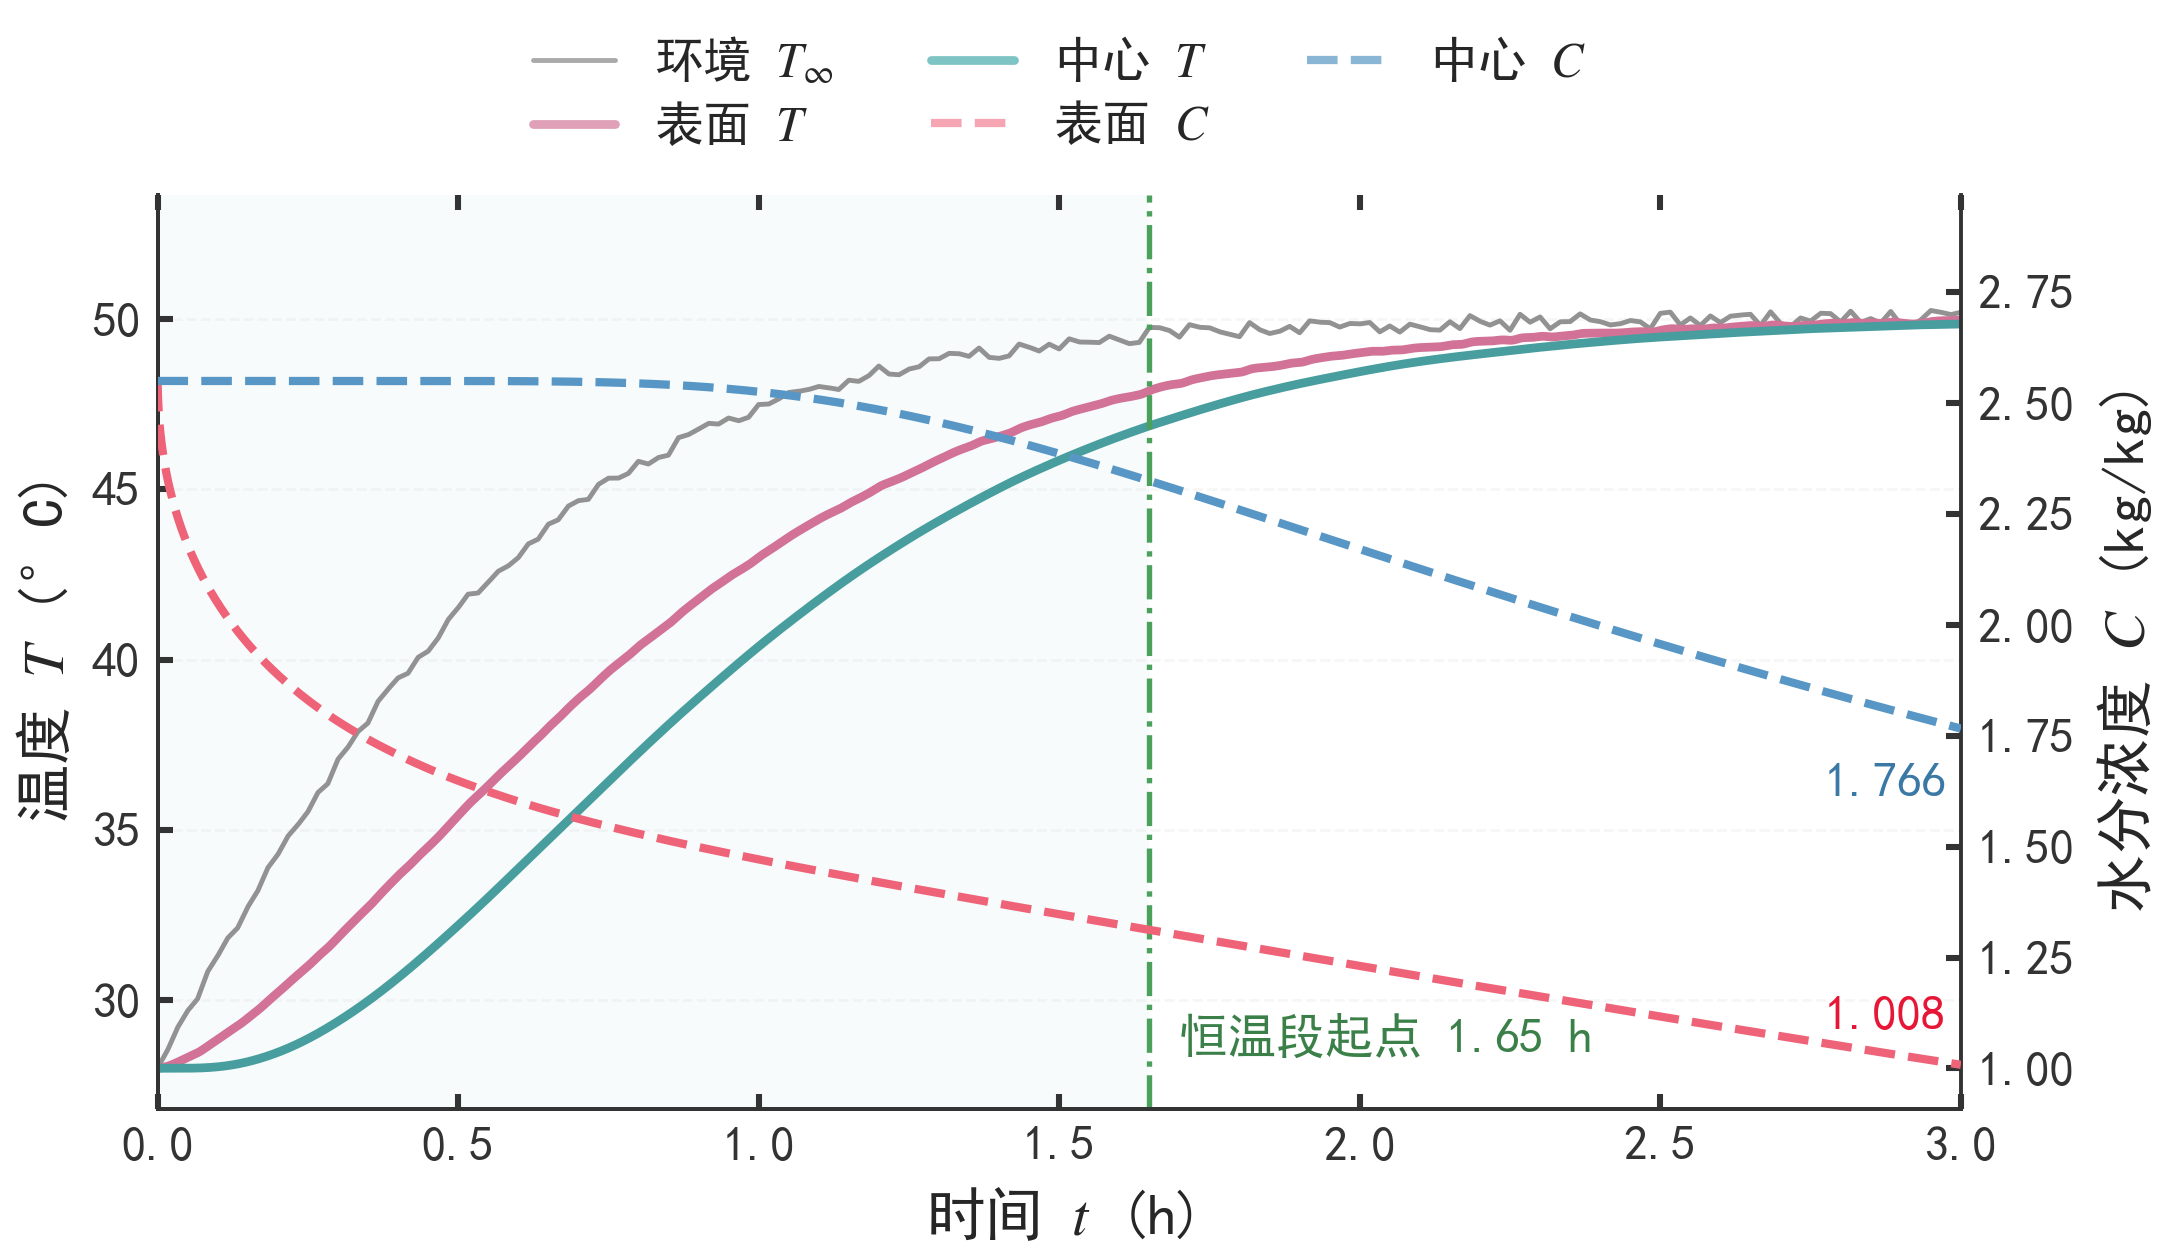
\includegraphics[width=0.90\textwidth]{figures/fig_q2_stage_transition.png}
  \caption{升温段与恒温段的演化分界}
  \label{fig:q2_stage_transition}
\end{figure}

\begin{figure}[H]
  \centering
  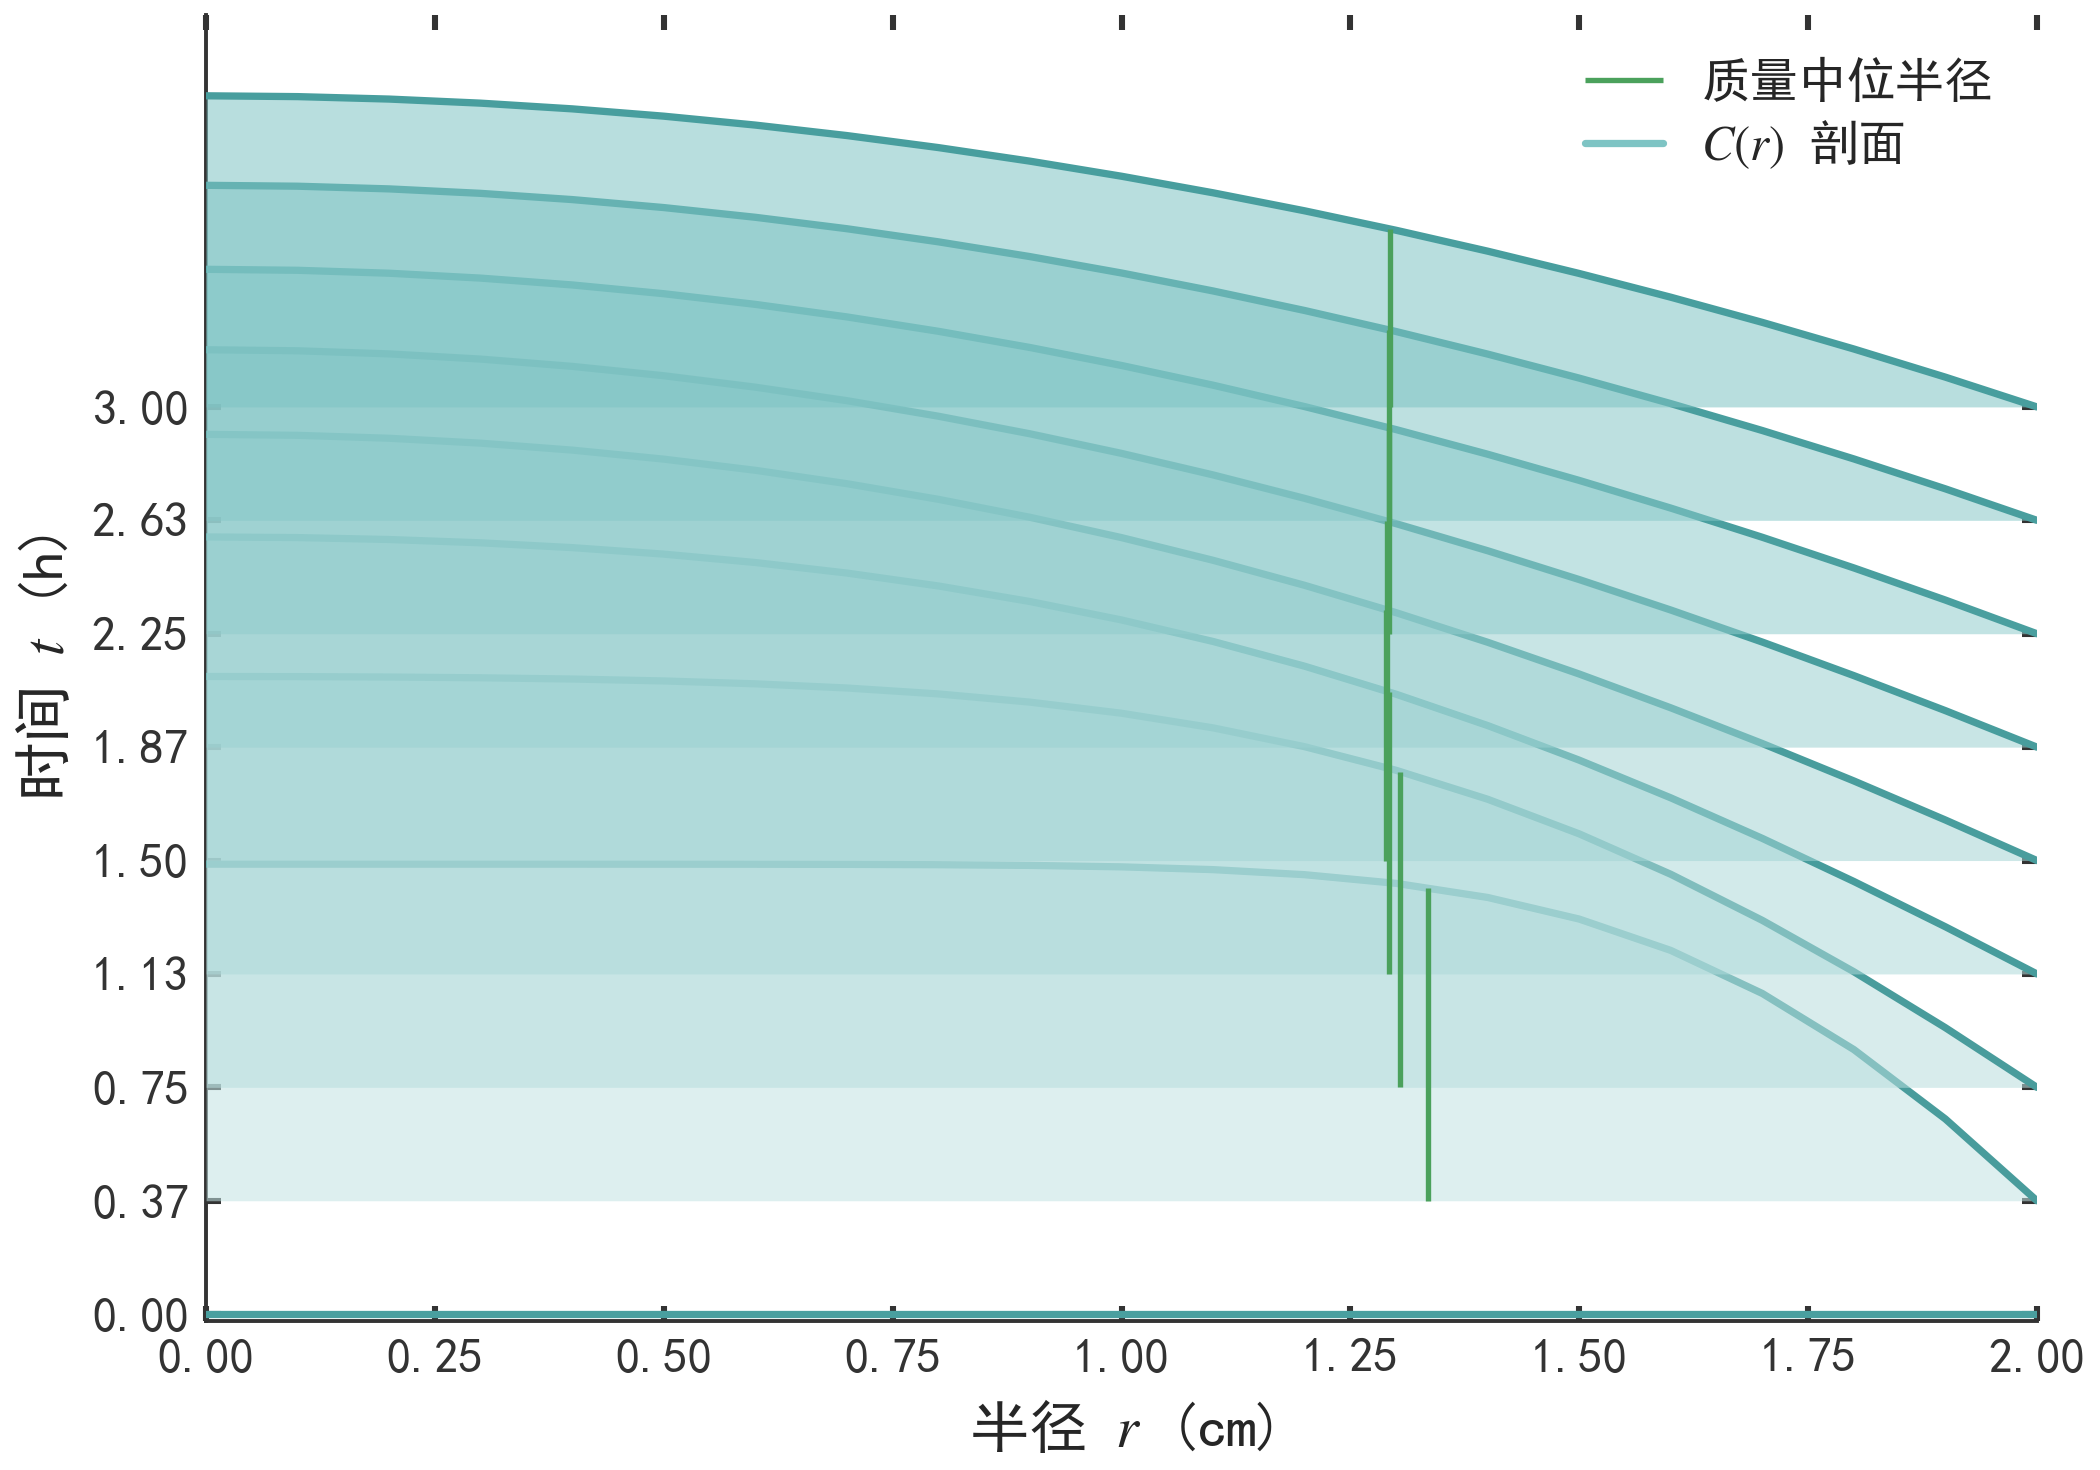
\includegraphics[width=0.86\textwidth]{figures/fig_q2_moist_ridgeline.png}
  \caption{水分径向分布的堆叠演化}
  \label{fig:q2_moist_ridgeline}
\end{figure}

\begin{figure}[H]
  \centering
  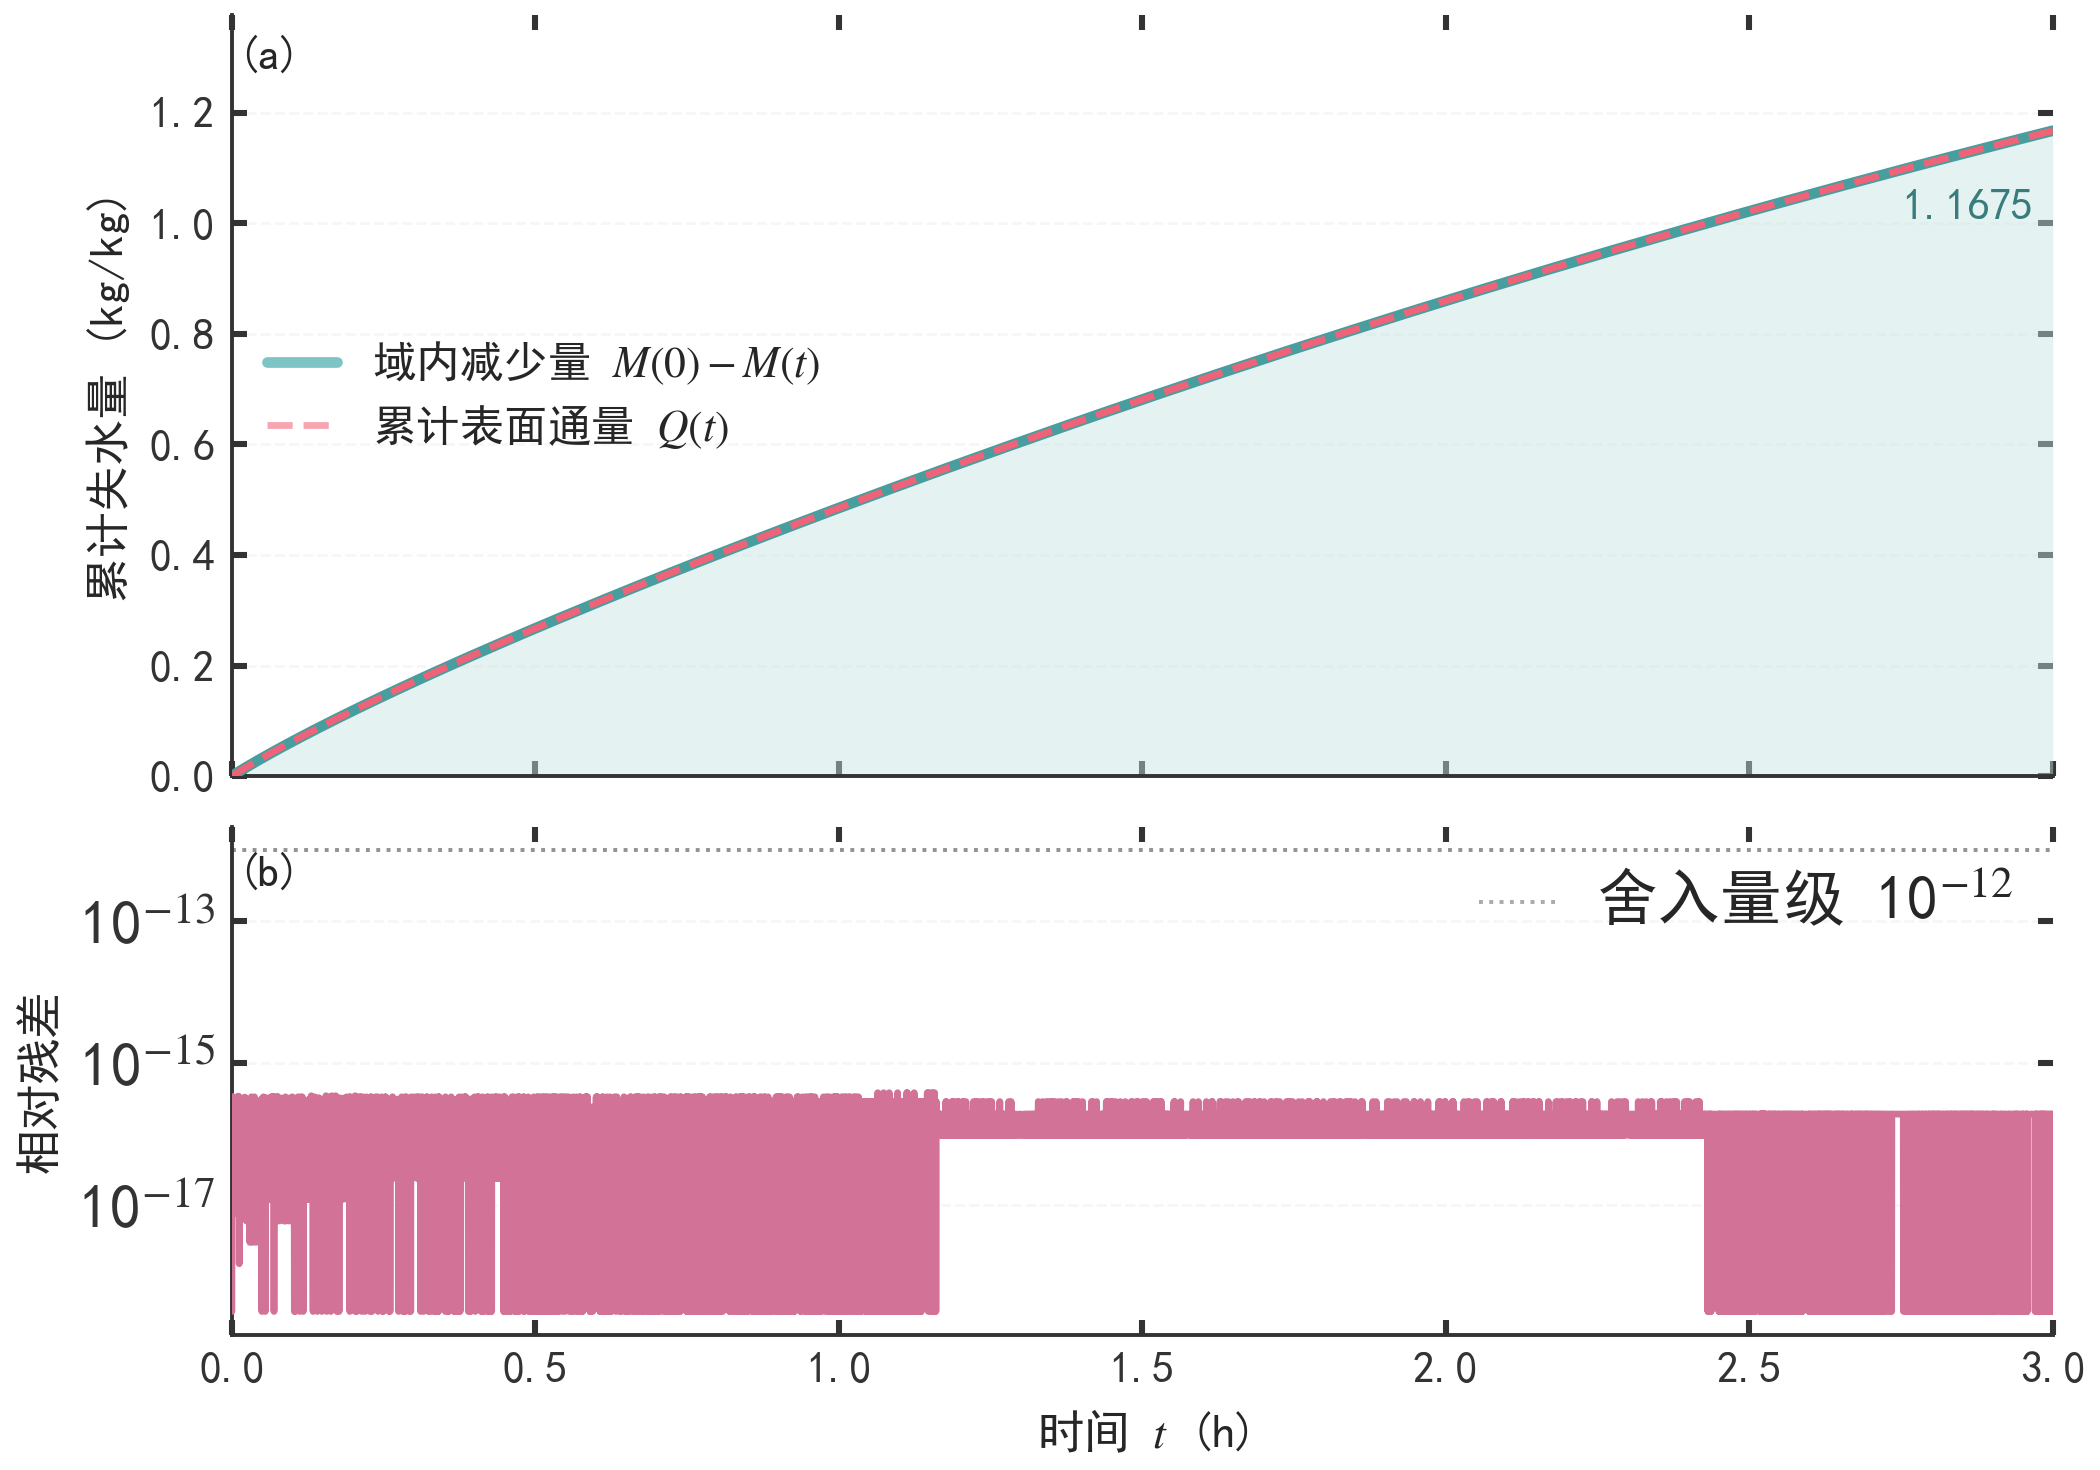
\includegraphics[width=0.86\textwidth]{figures/fig_q2_flux_balance.png}
  \caption{累计失水通量与守恒残差}
  \label{fig:q2_flux_balance}
\end{figure}

% ── 问题 3 ────────────────────────────────────────────────────
\begin{figure}[H]
  \centering
  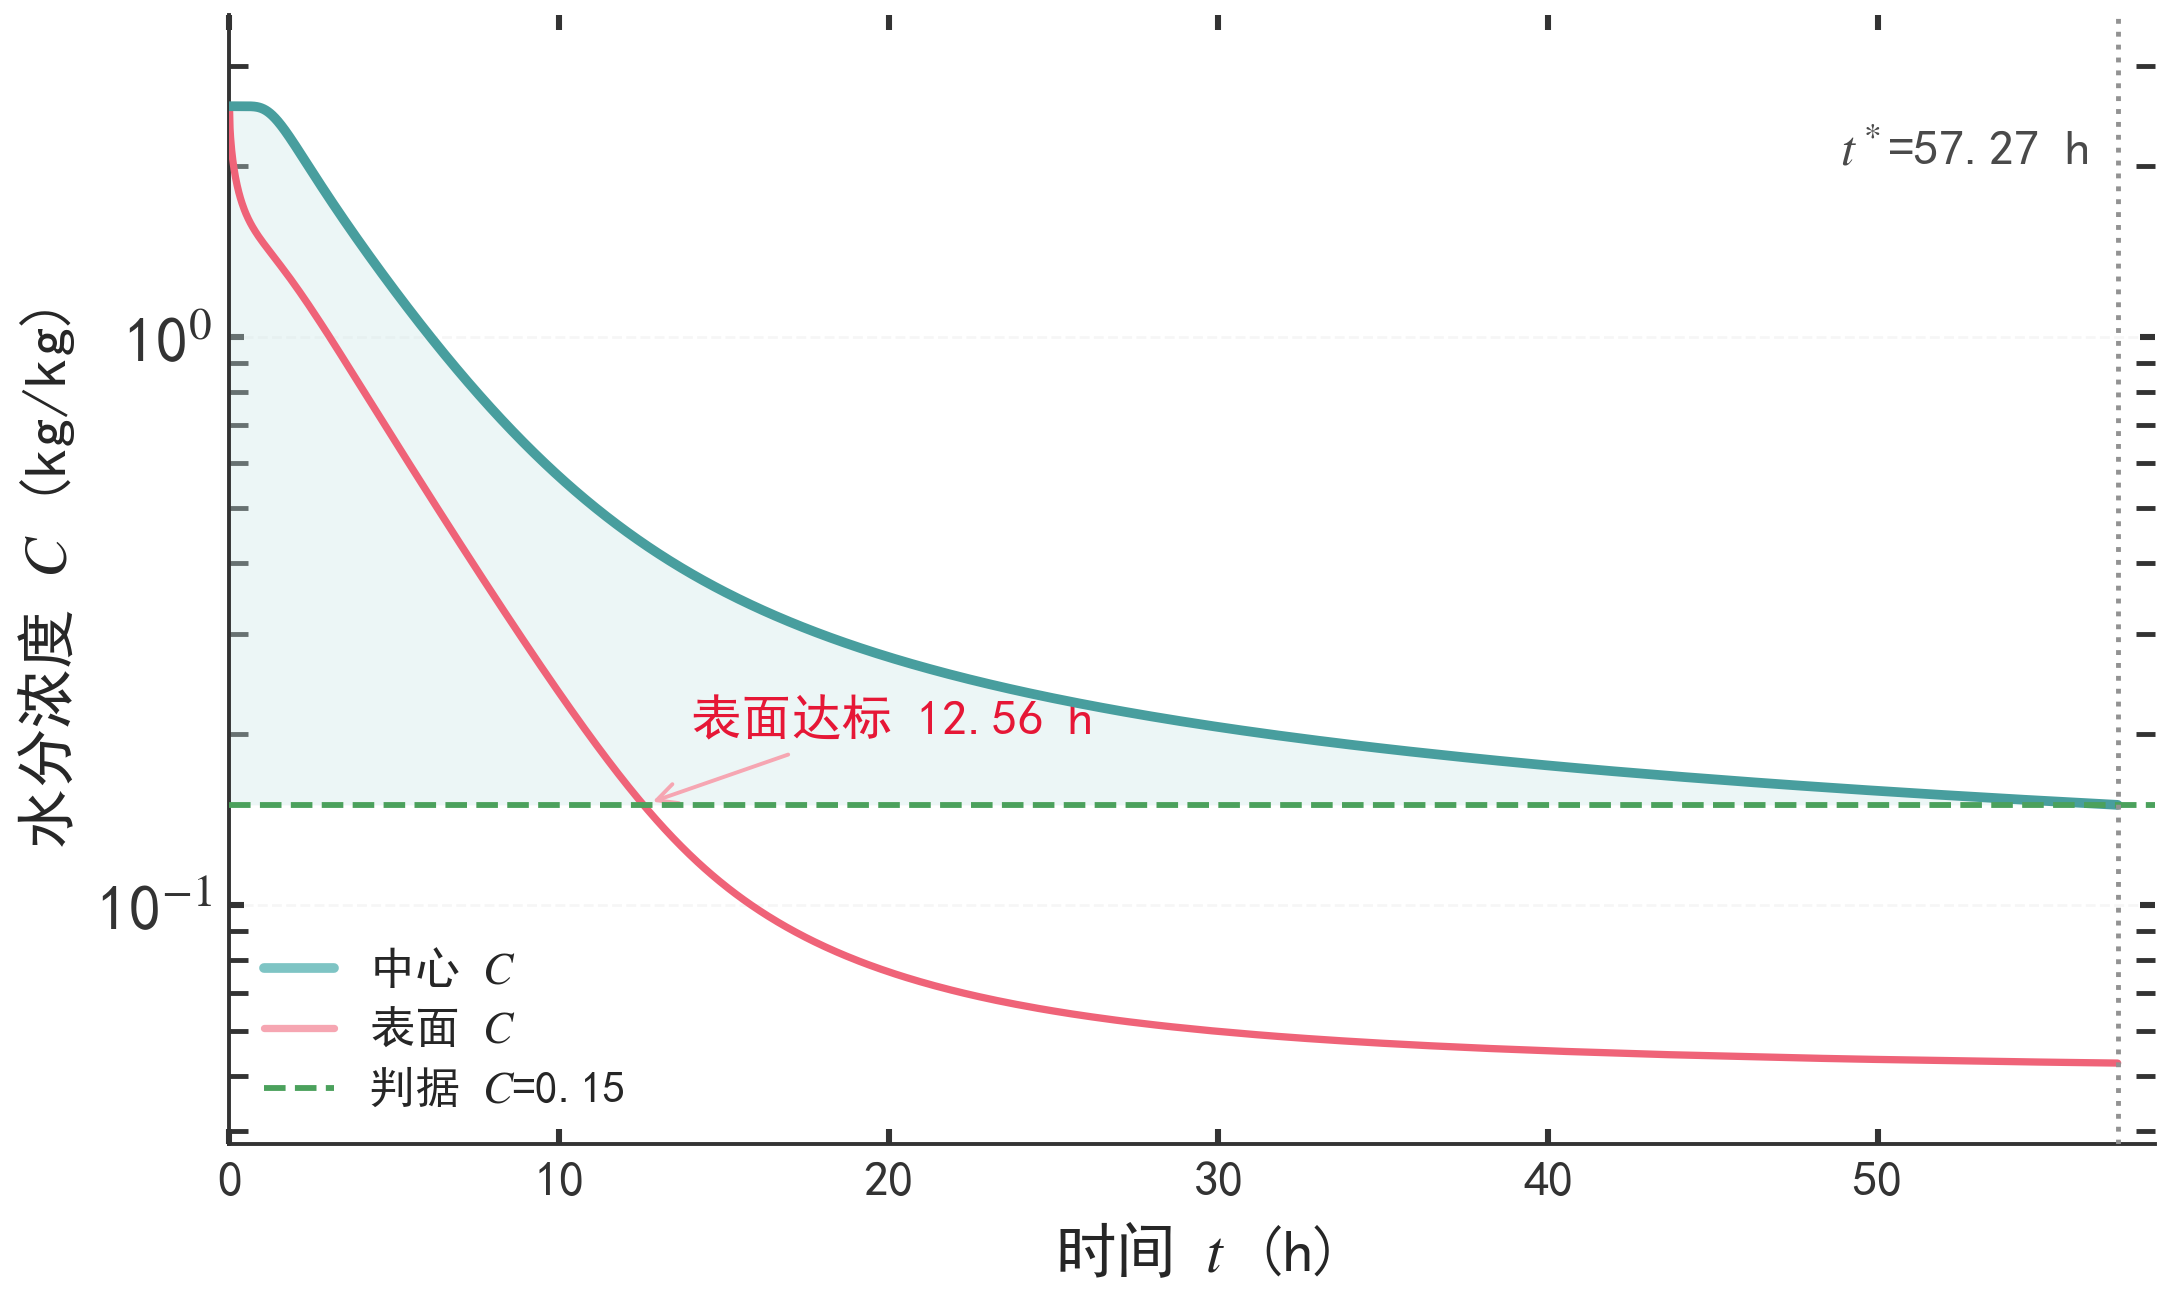
\includegraphics[width=0.90\textwidth]{figures/fig_q3_center_decay.png}
  \caption{中心含水率长时程衰减}
  \label{fig:q3_center_decay}
\end{figure}

\begin{figure}[H]
  \centering
  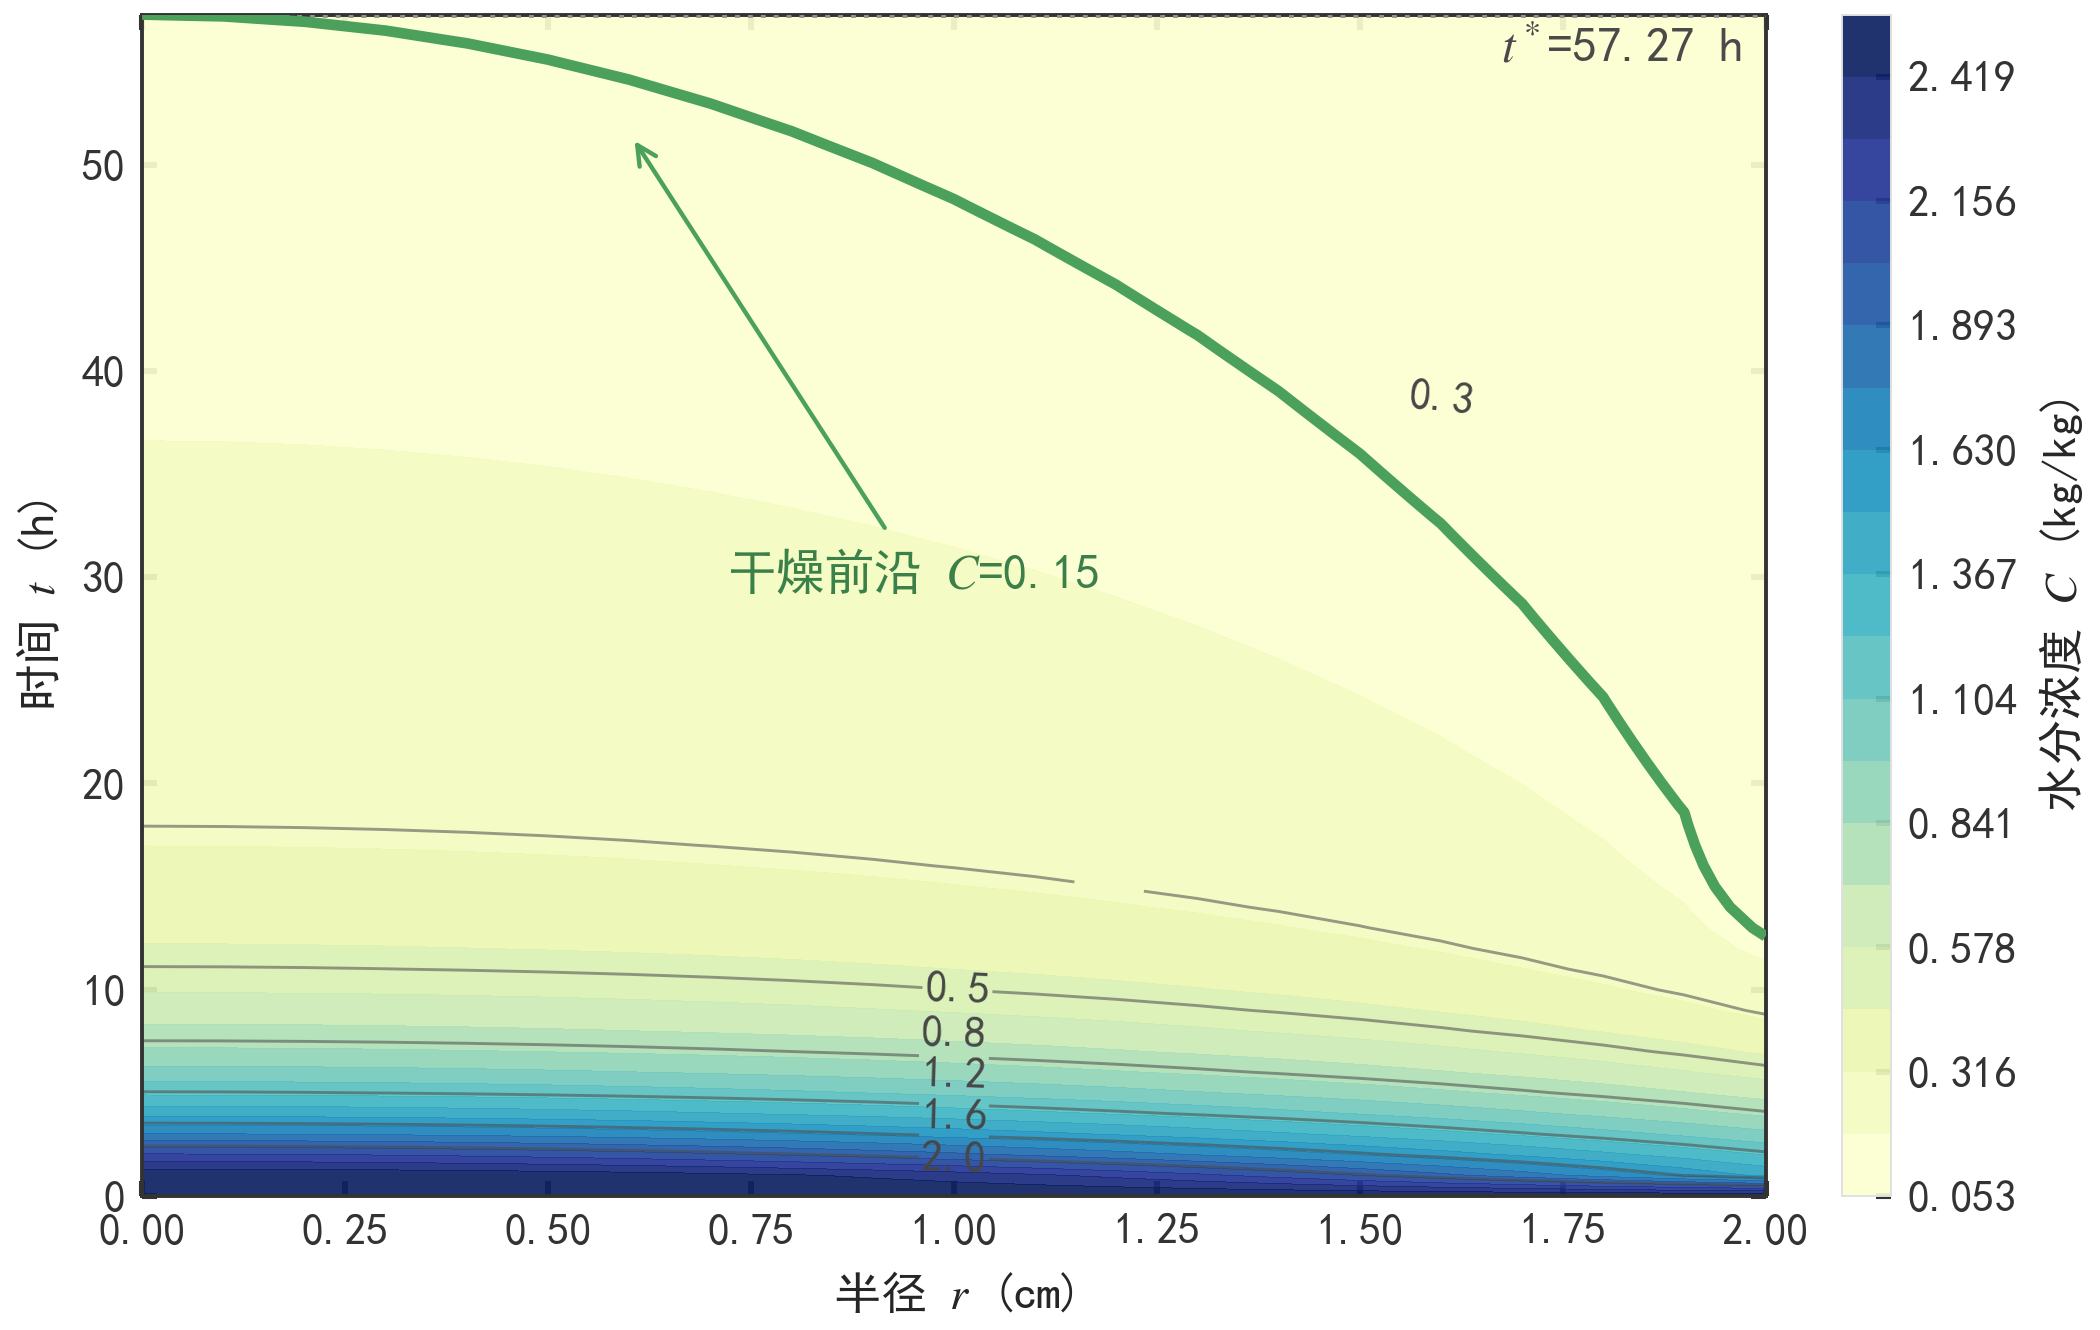
\includegraphics[width=0.86\textwidth]{figures/fig_q3_threshold_contour.png}
  \caption{干燥前沿在 $r$–$t$ 平面的推进}
  \label{fig:q3_threshold_contour}
\end{figure}

\begin{figure}[H]
  \centering
  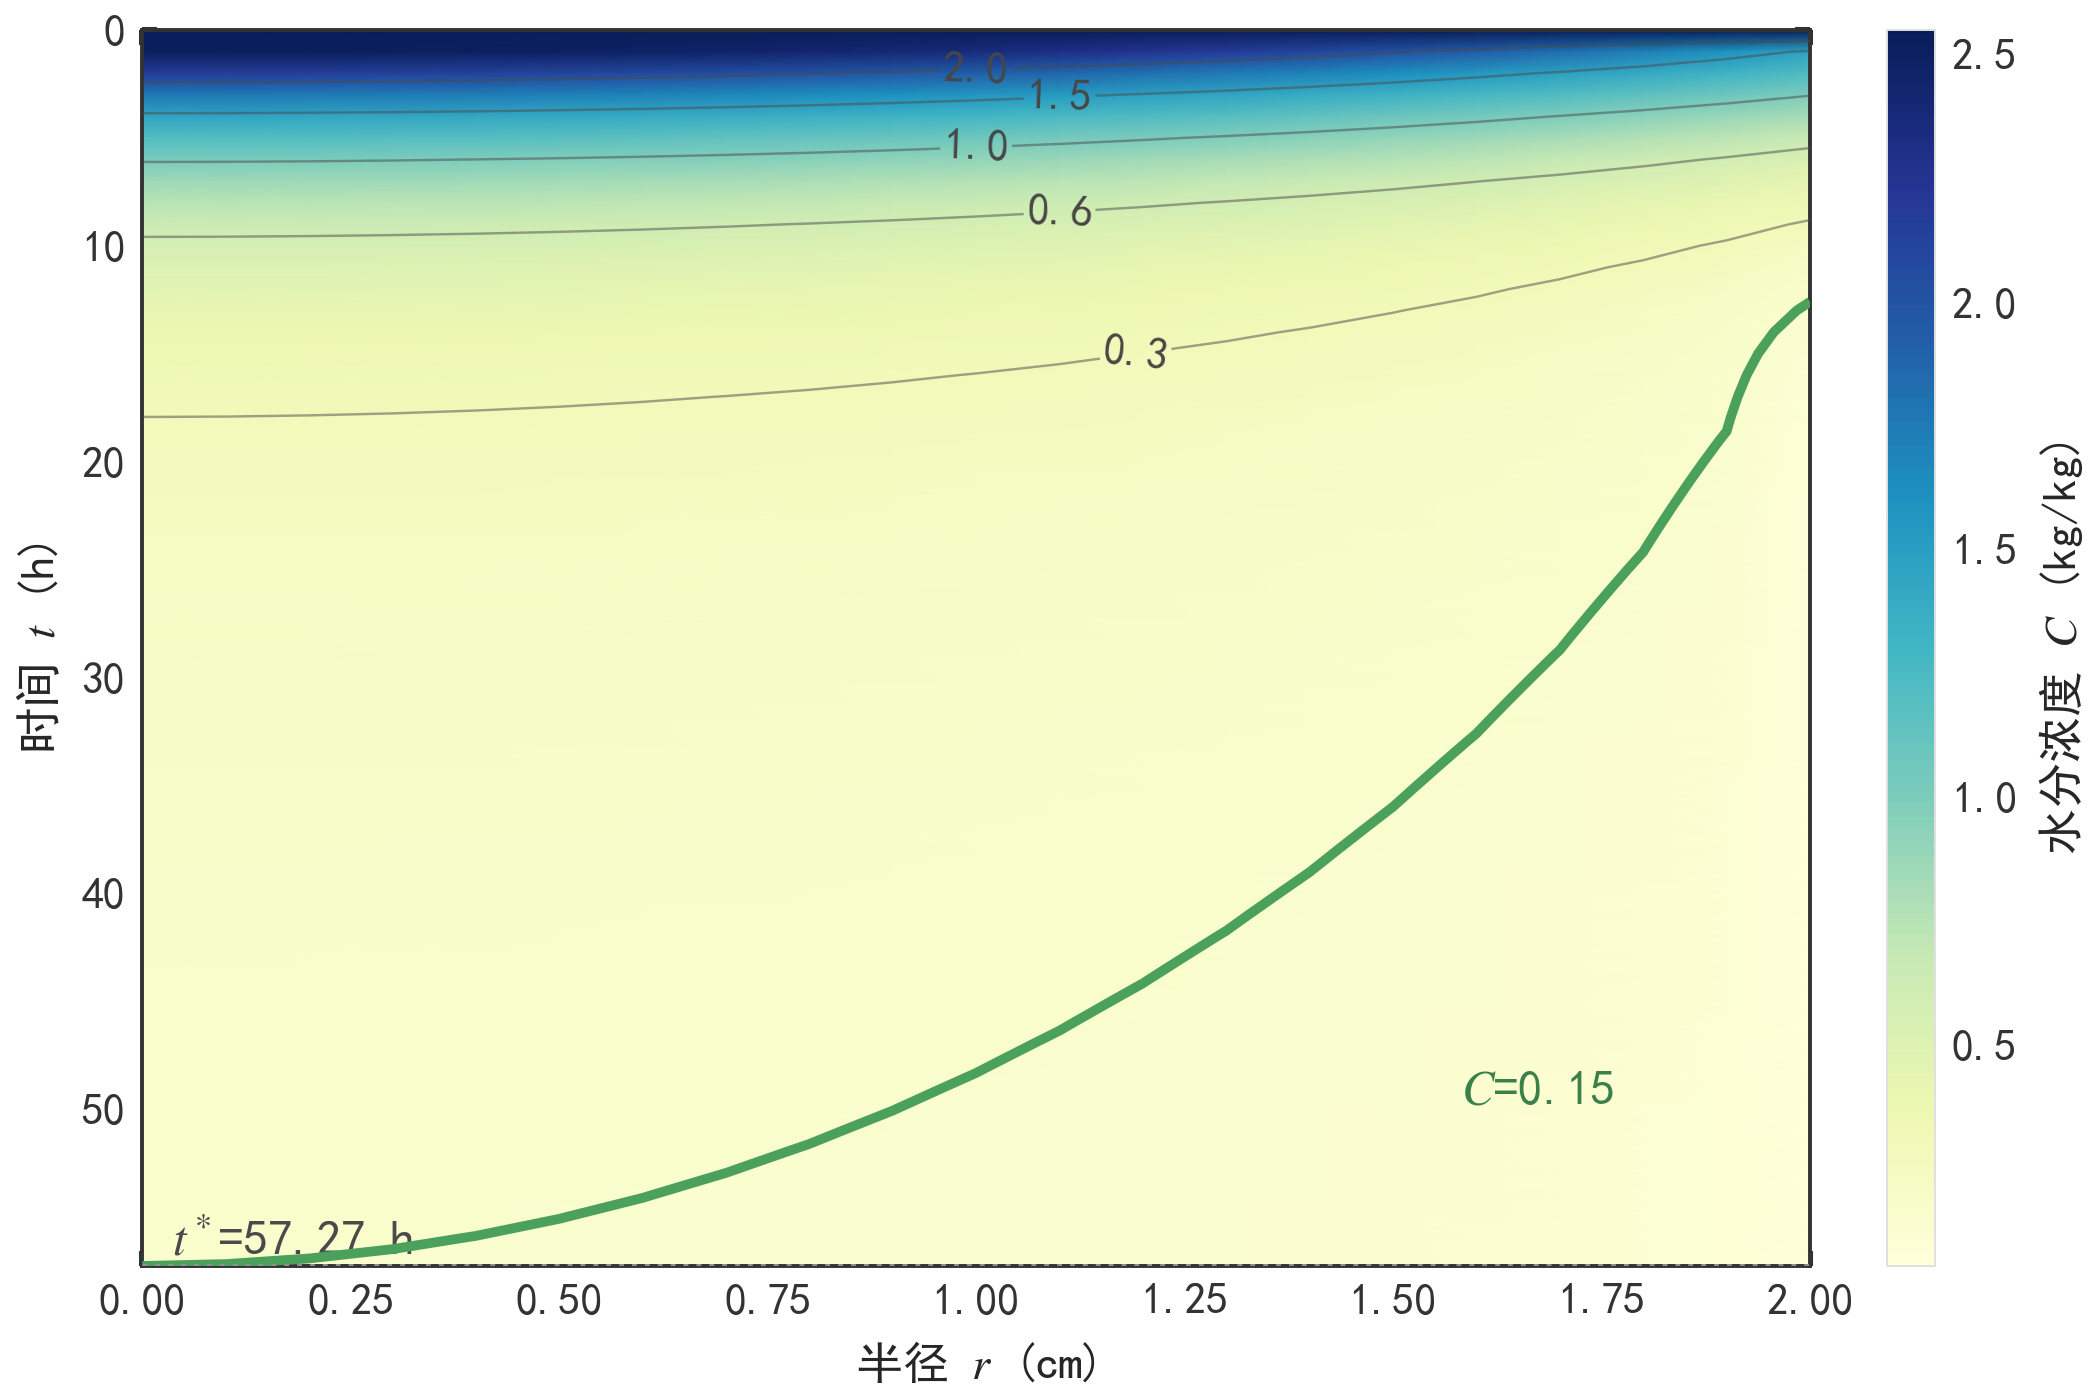
\includegraphics[width=0.86\textwidth]{figures/fig_q3_hovmoller.png}
  \caption{全时程水分场时空图}
  \label{fig:q3_hovmoller}
\end{figure}

% ── 问题 4 与对比 ─────────────────────────────────────────────
\begin{figure}[H]
  \centering
  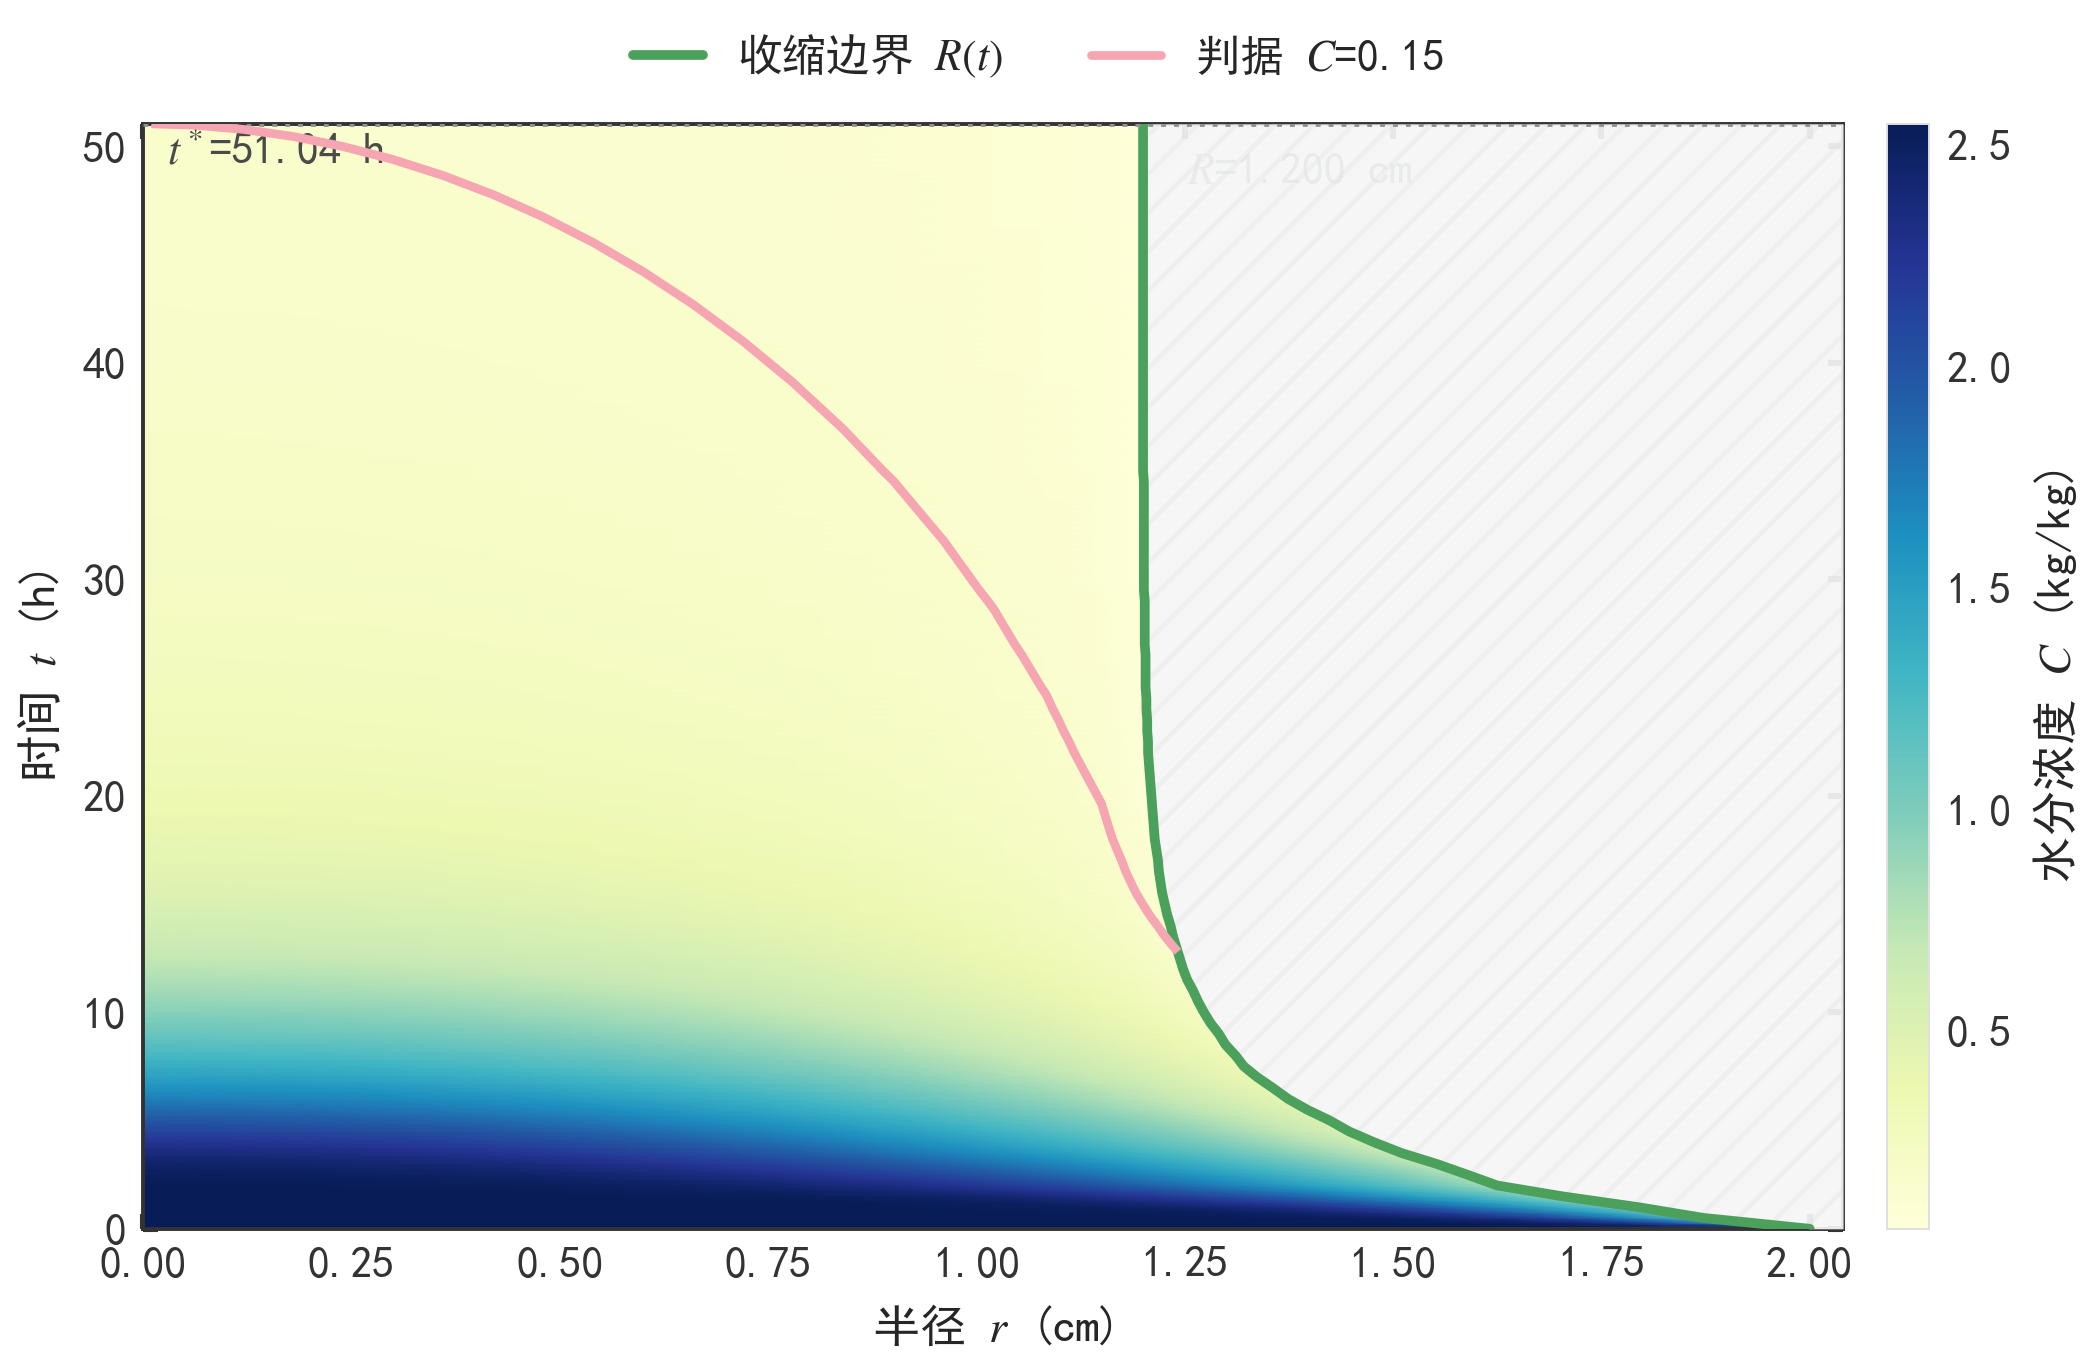
\includegraphics[width=0.86\textwidth]{figures/fig_q4_moving_domain_heatmap.png}
  \caption{收缩域上的水分时空分布}
  \label{fig:q4_moving_domain_heatmap}
\end{figure}

\begin{figure}[H]
  \centering
  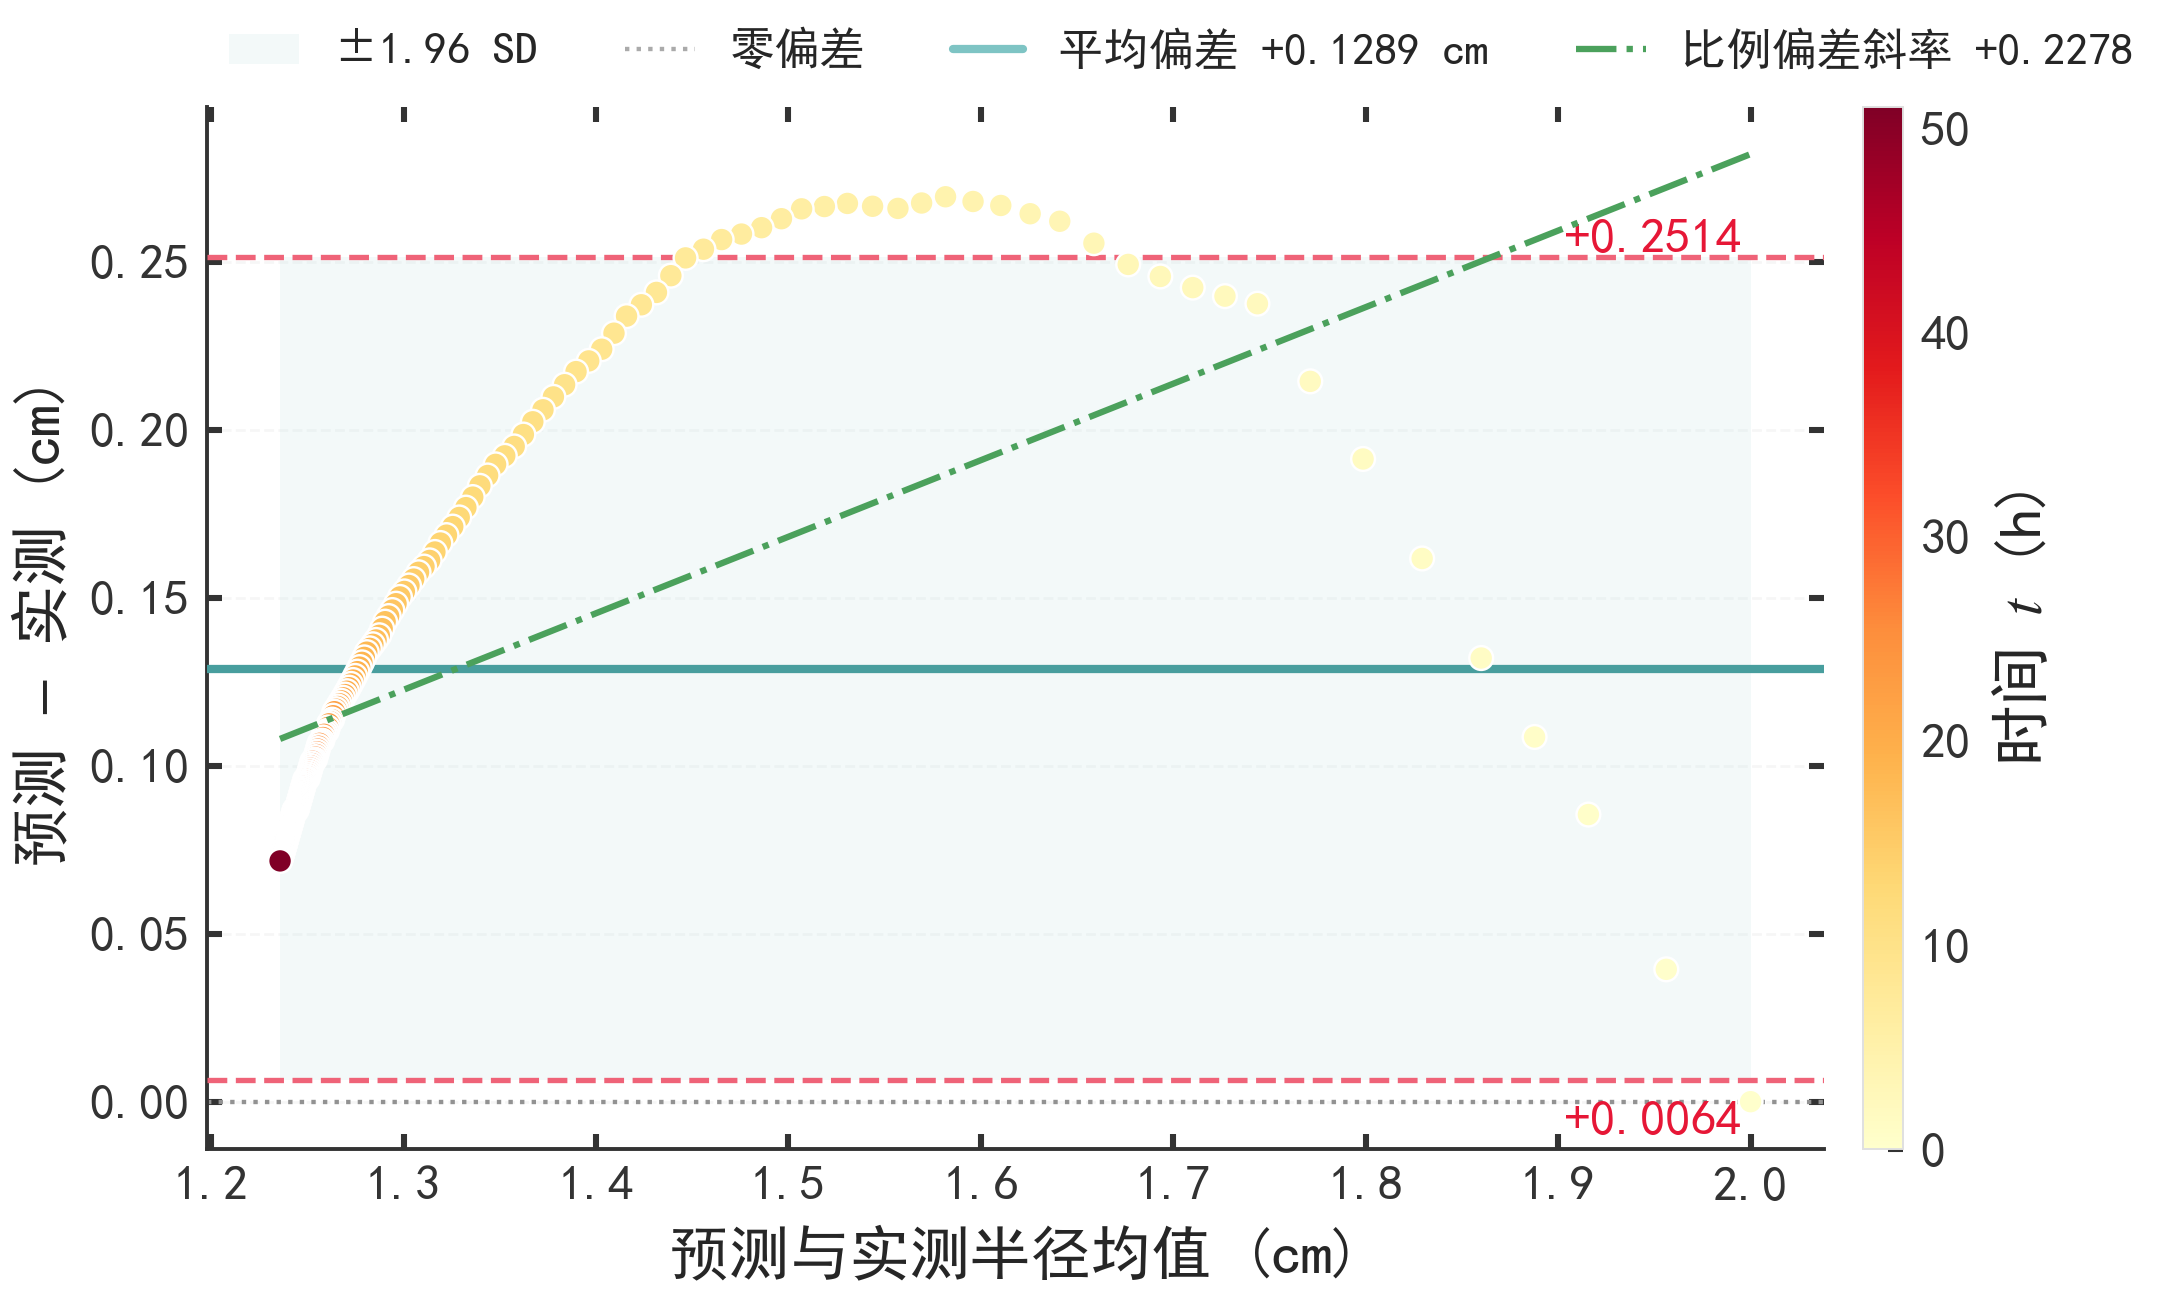
\includegraphics[width=0.90\textwidth]{figures/fig_q4_shrink_validation.png}
  \caption{预测半径与实测半径的一致性}
  \label{fig:q4_shrink_validation}
\end{figure}

\begin{figure}[H]
  \centering
  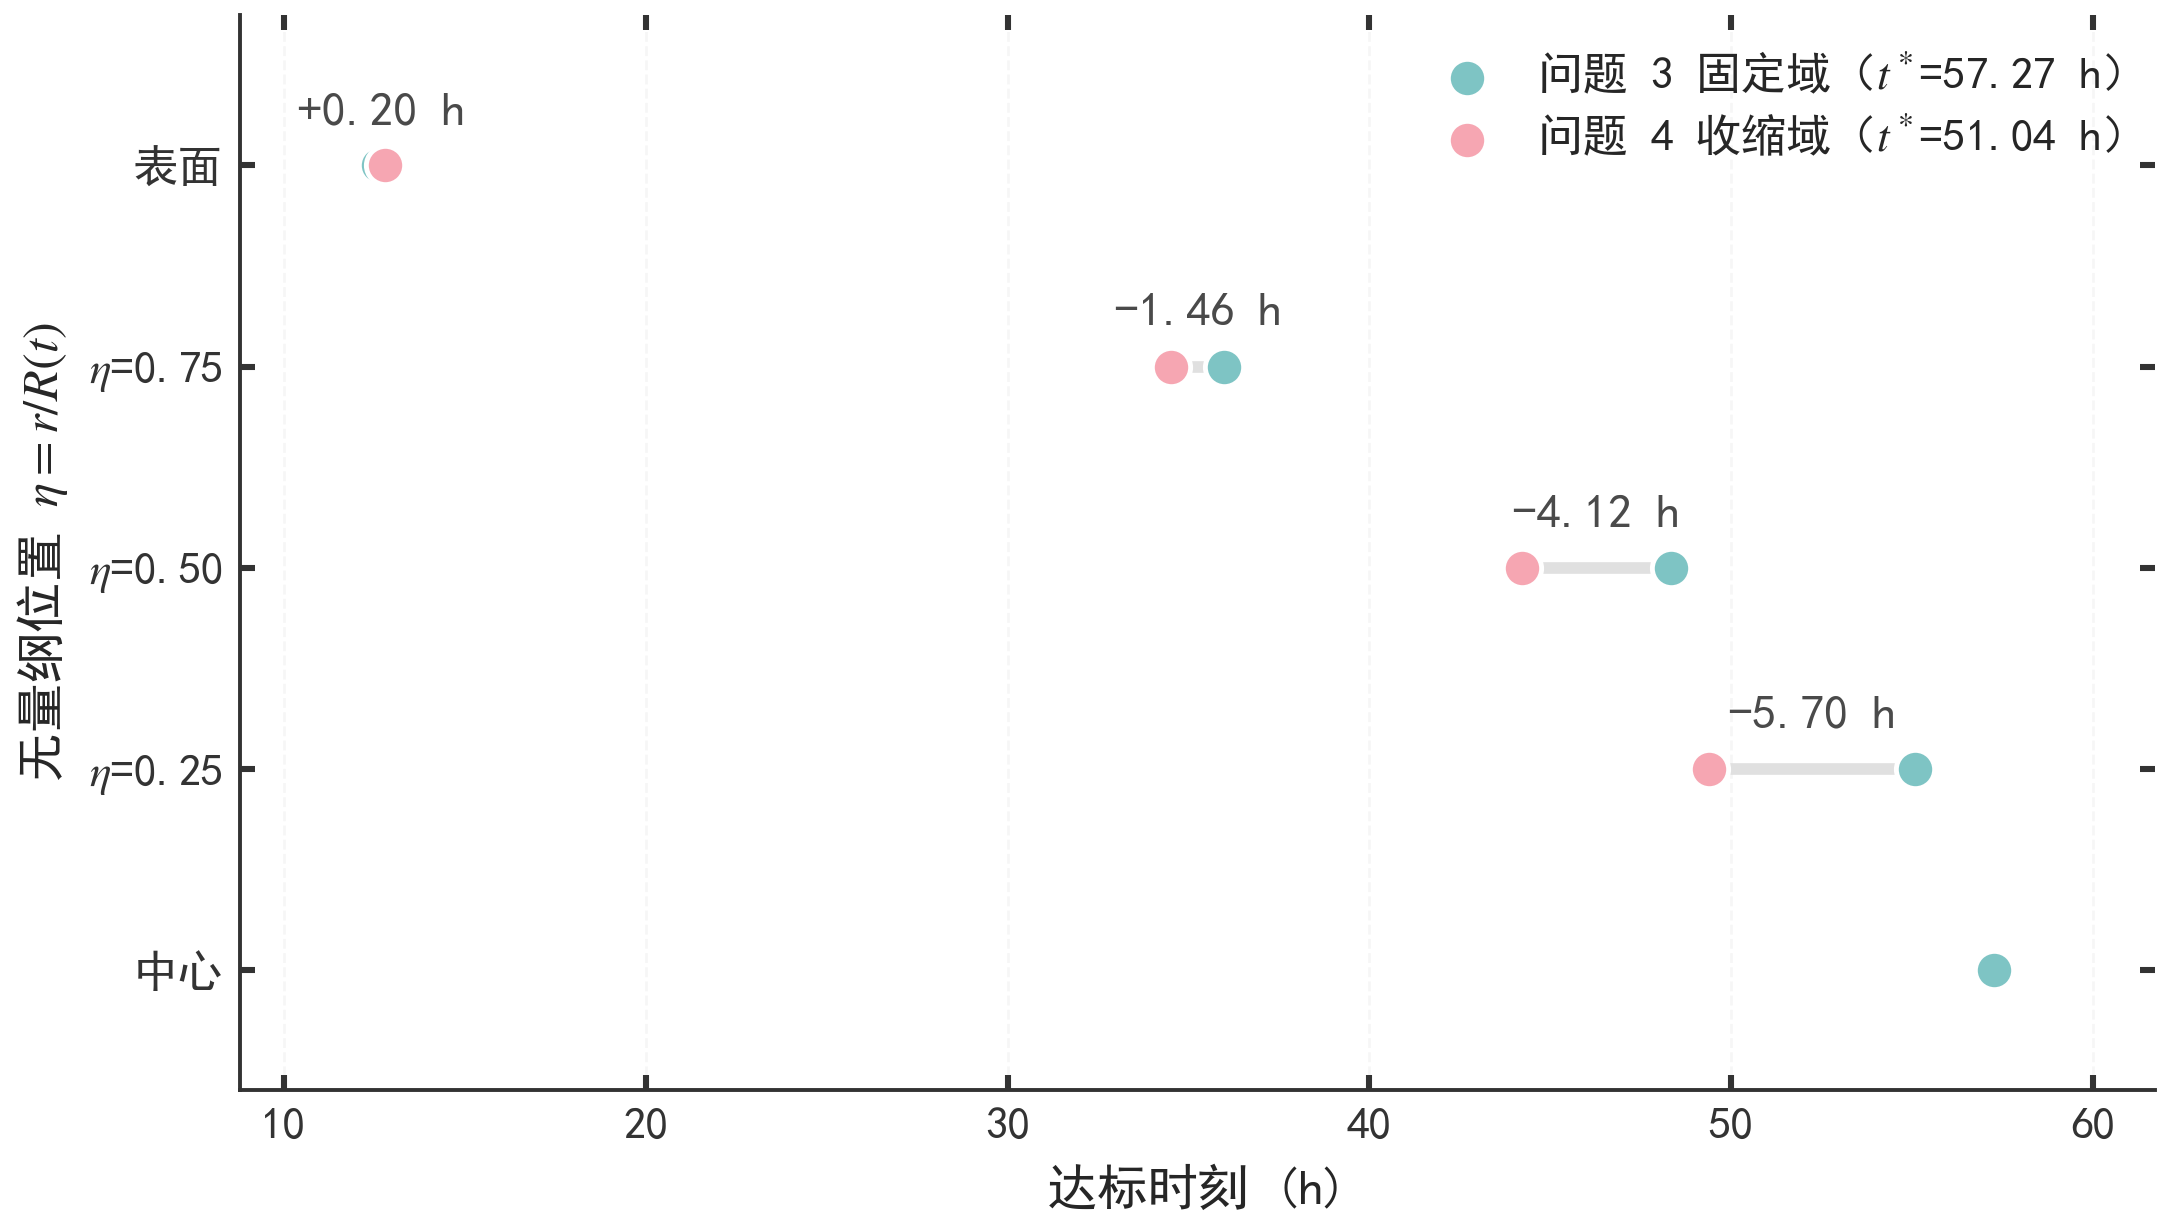
\includegraphics[width=0.90\textwidth]{figures/fig_q34_compare_dumbbell.png}
  \caption{固定域与收缩域达标时刻对比}
  \label{fig:q34_compare_dumbbell}
\end{figure}

% ── 稳健性 ────────────────────────────────────────────────────
\begin{figure}[H]
  \centering
  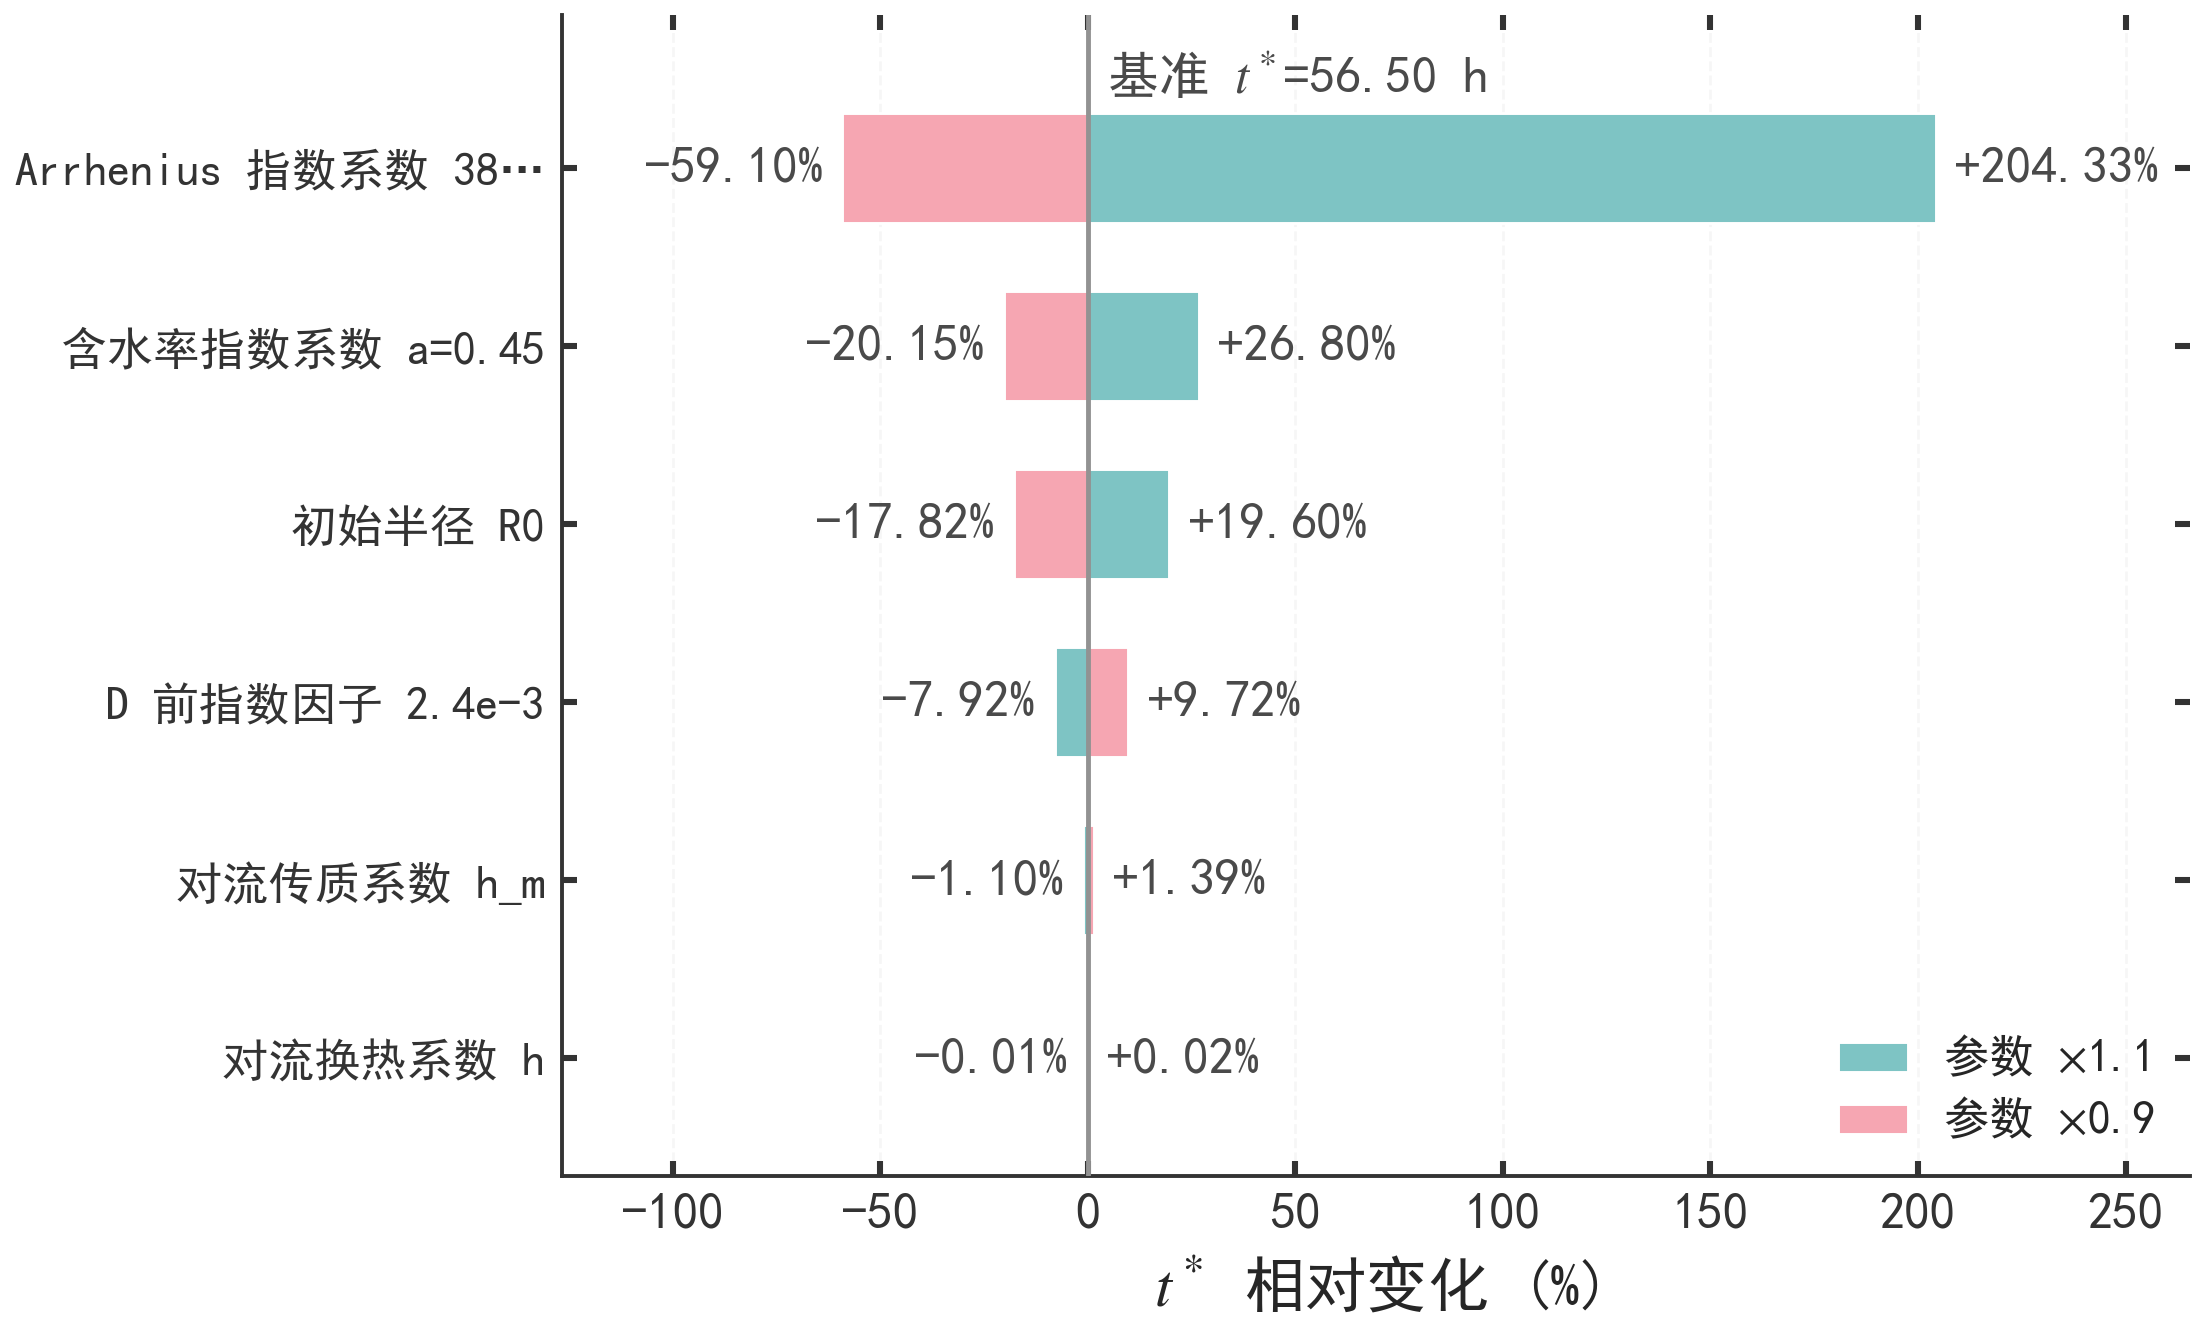
\includegraphics[width=0.92\textwidth]{figures/fig_sensitivity_tornado.png}
  \caption{参数对烘干时长的敏感性排序}
  \label{fig:sensitivity_tornado}
\end{figure}

\begin{figure}[H]
  \centering
  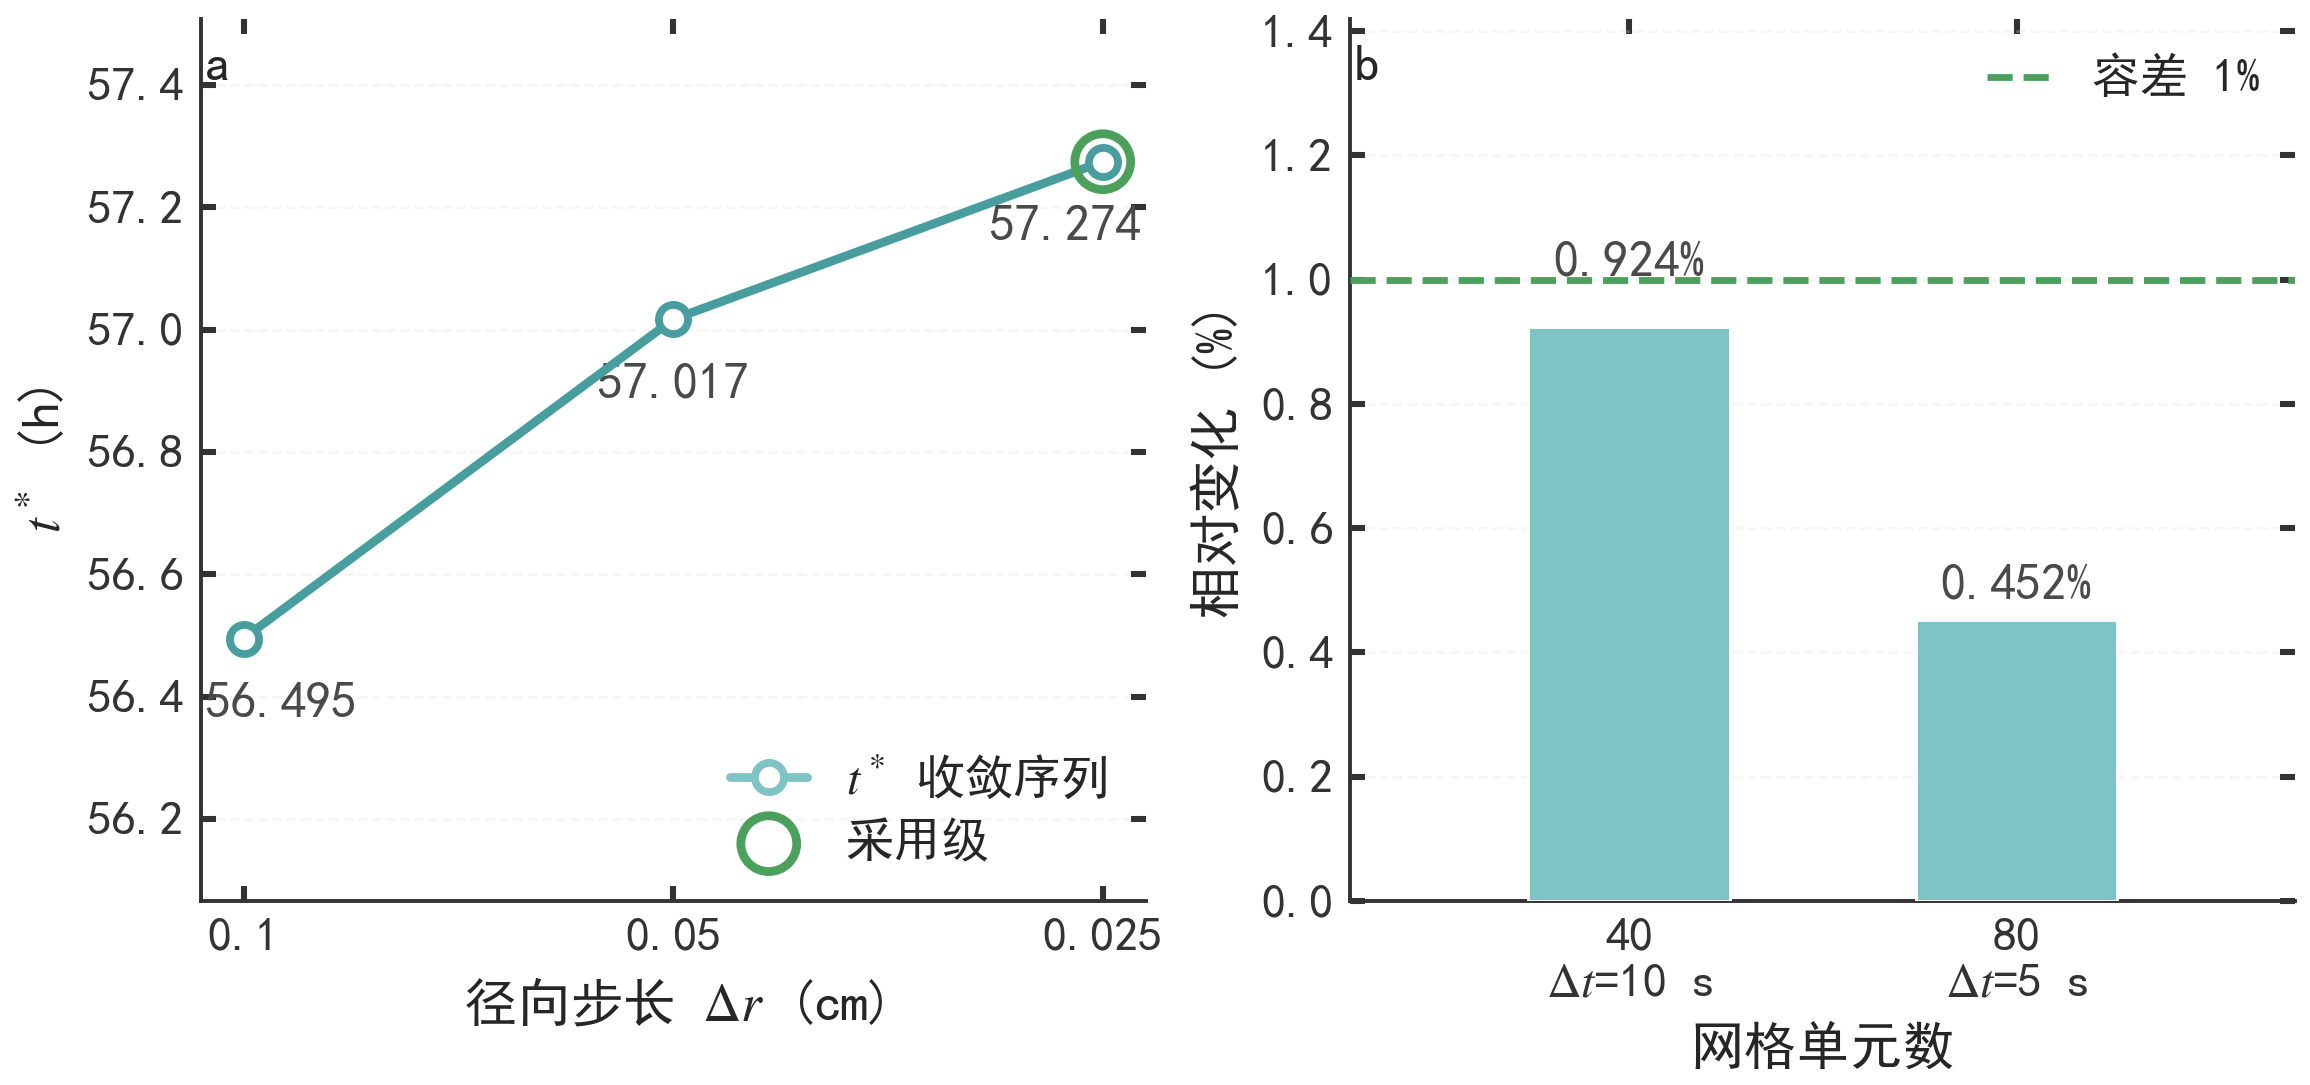
\includegraphics[width=0.96\textwidth]{figures/fig_grid_convergence.png}
  \caption{网格与时间步收敛性}
  \label{fig:grid_convergence}
\end{figure}

% ── 技术路线与流程（HTML 矢量图，插入 PDF）────────────────────
\begin{figure}[H]
  \centering
  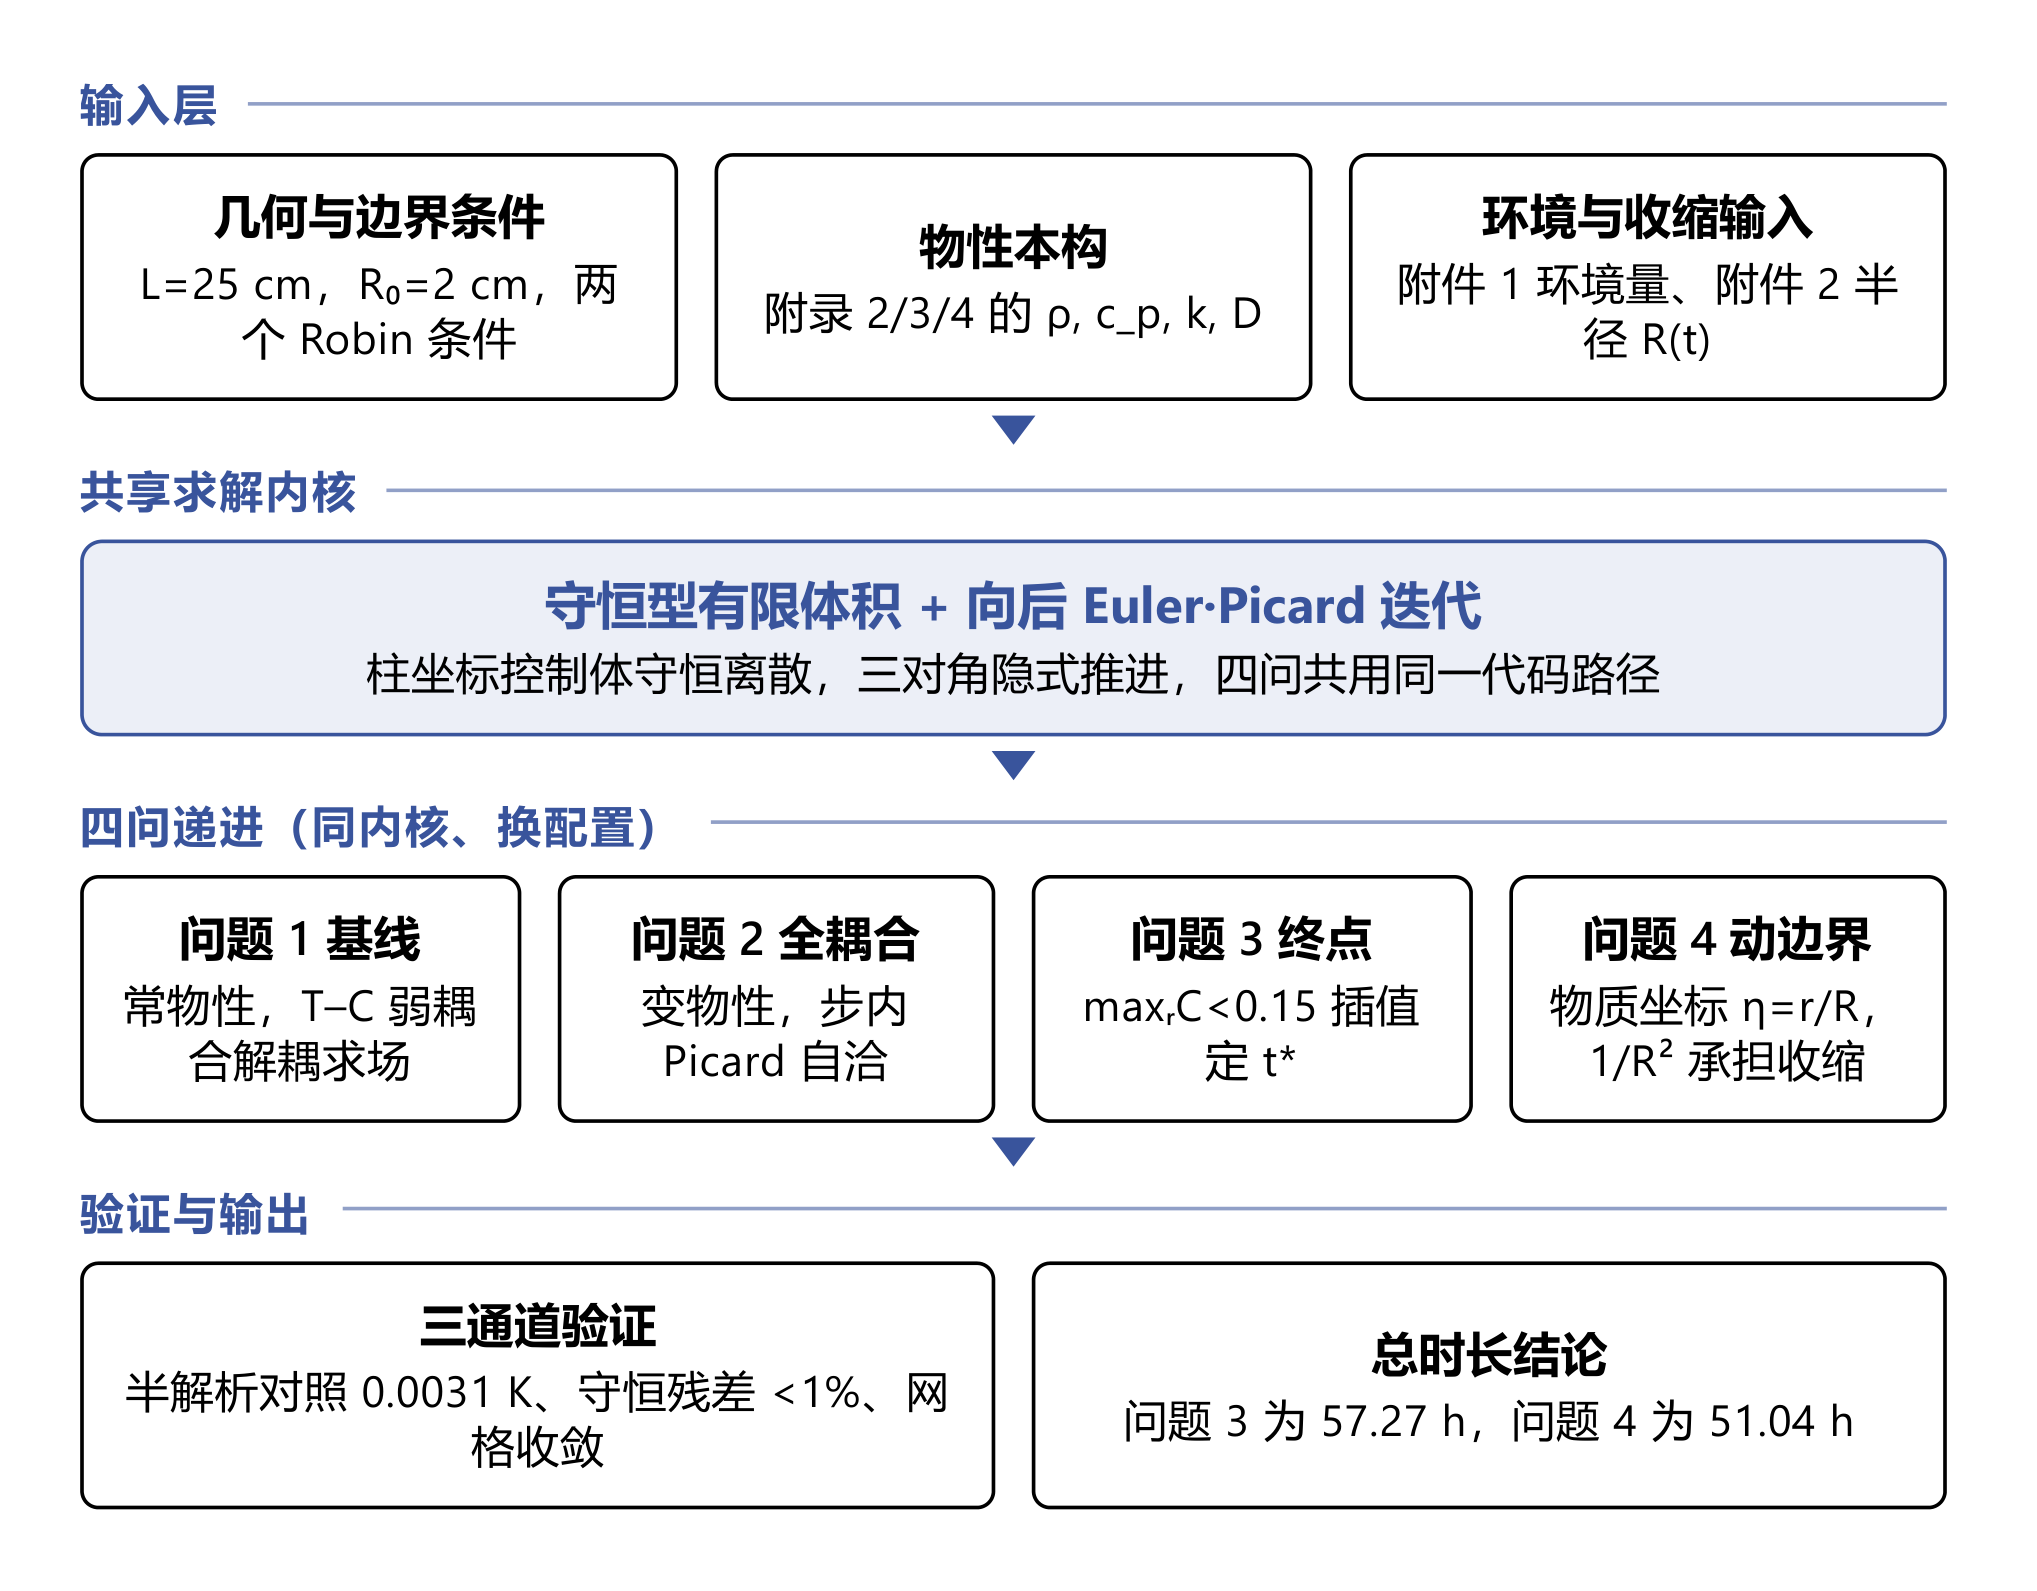
\includegraphics[width=0.96\textwidth,height=0.8\textheight,keepaspectratio]{figures/fig_roadmap.pdf}
  \caption{总体技术路线：四问递进与共用求解内核}
  \label{fig:roadmap}
\end{figure}

\begin{figure}[H]
  \centering
  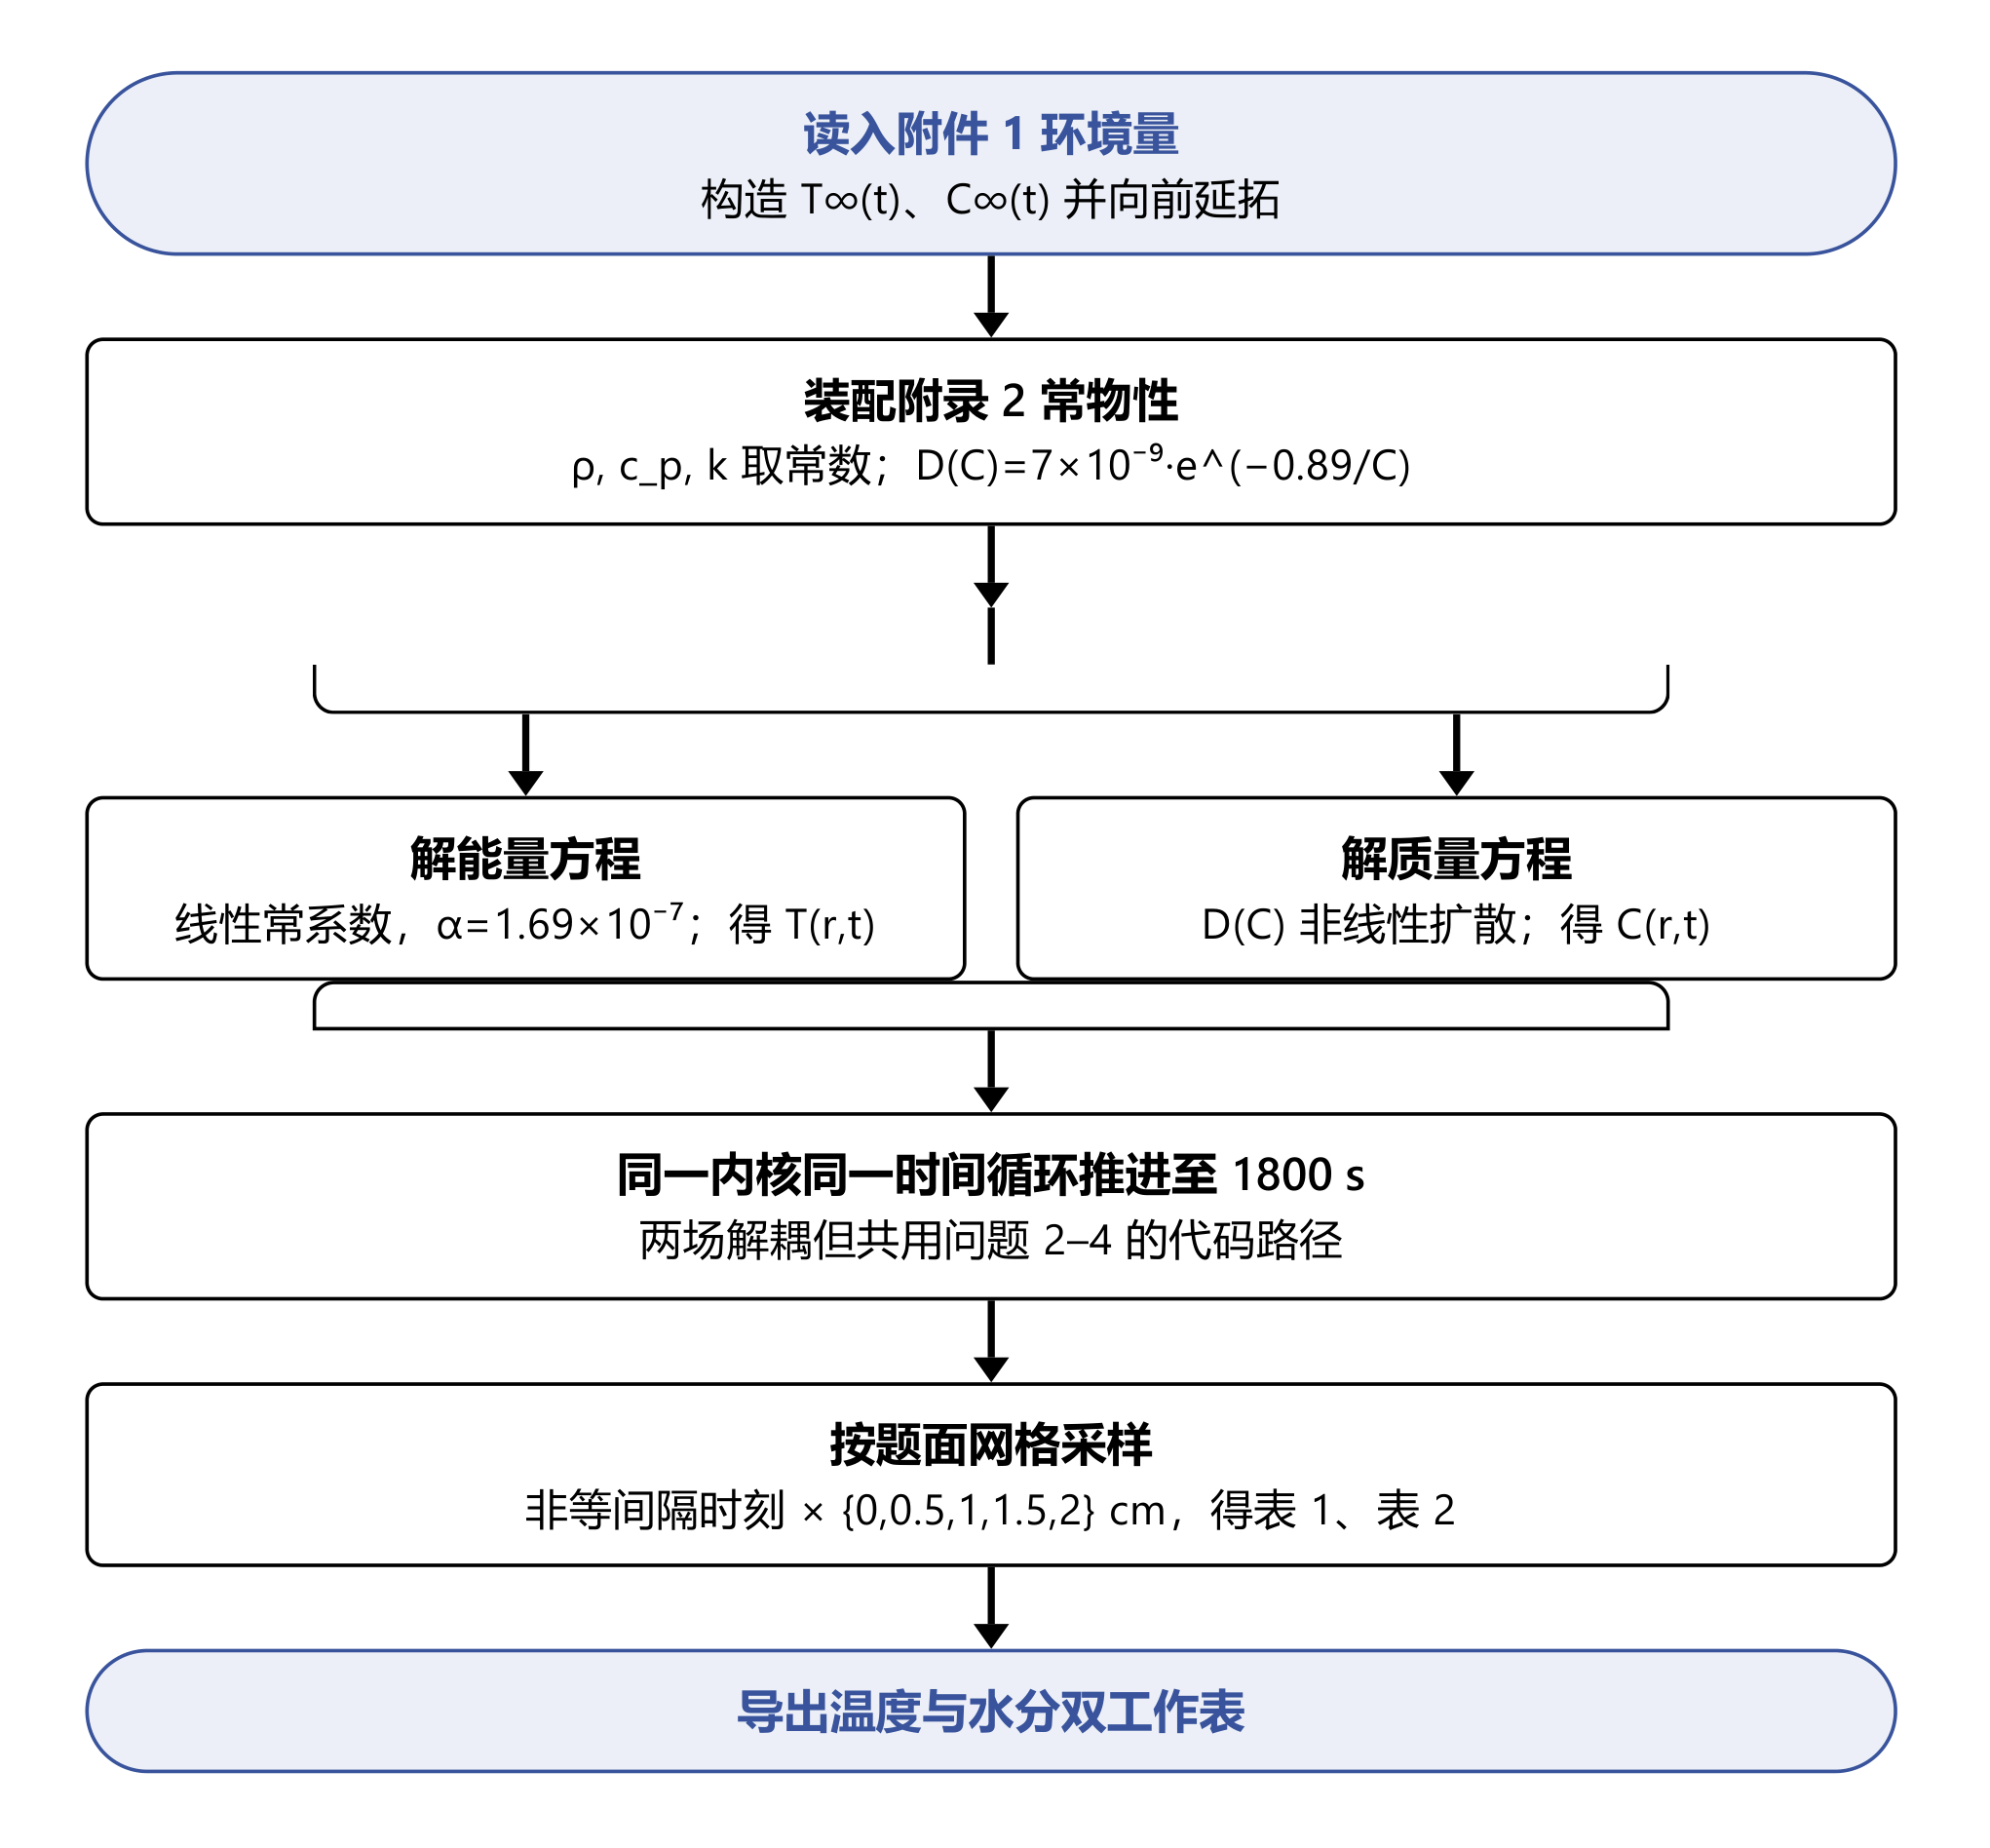
\includegraphics[width=0.96\textwidth,height=0.8\textheight,keepaspectratio]{figures/fig_flow_q1.pdf}
  \caption{问题 1 求解流程}
  \label{fig:flow_q1}
\end{figure}

\begin{figure}[H]
  \centering
  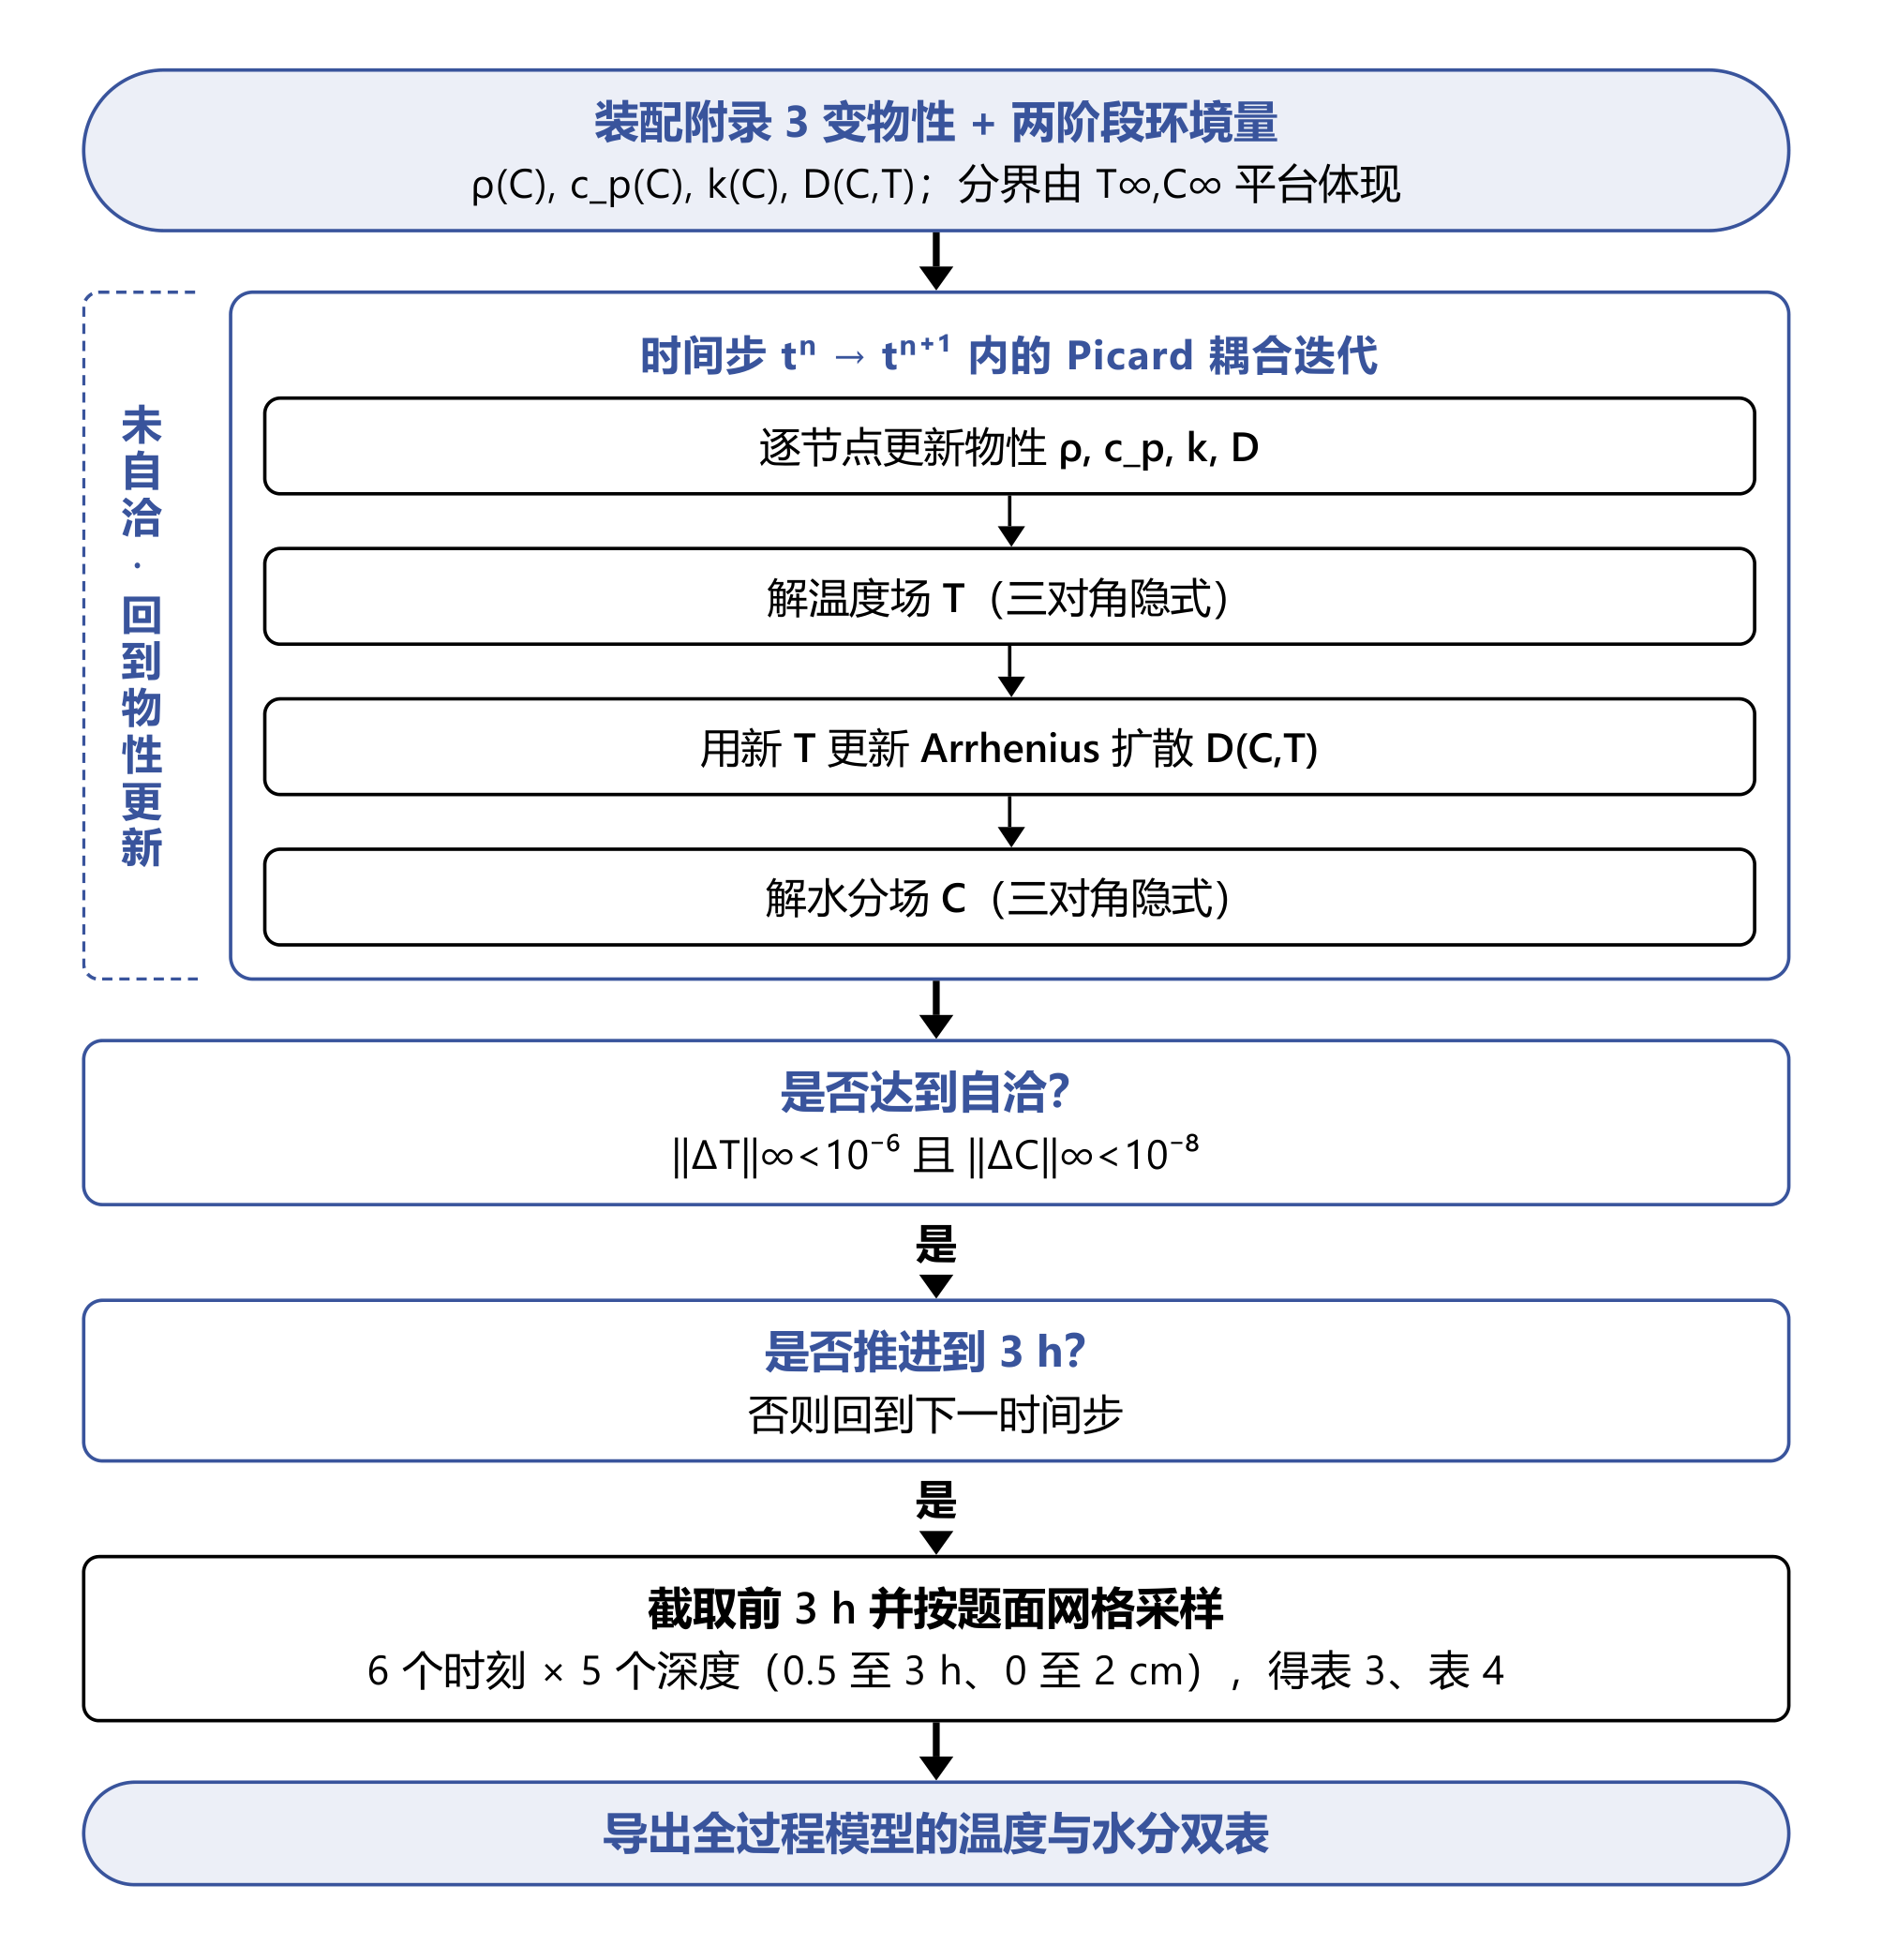
\includegraphics[width=0.94\textwidth,height=0.8\textheight,keepaspectratio]{figures/fig_flow_q2.pdf}
  \caption{问题 2 求解流程：变物性与步内 Picard 耦合迭代}
  \label{fig:flow_q2}
\end{figure}

\begin{figure}[H]
  \centering
  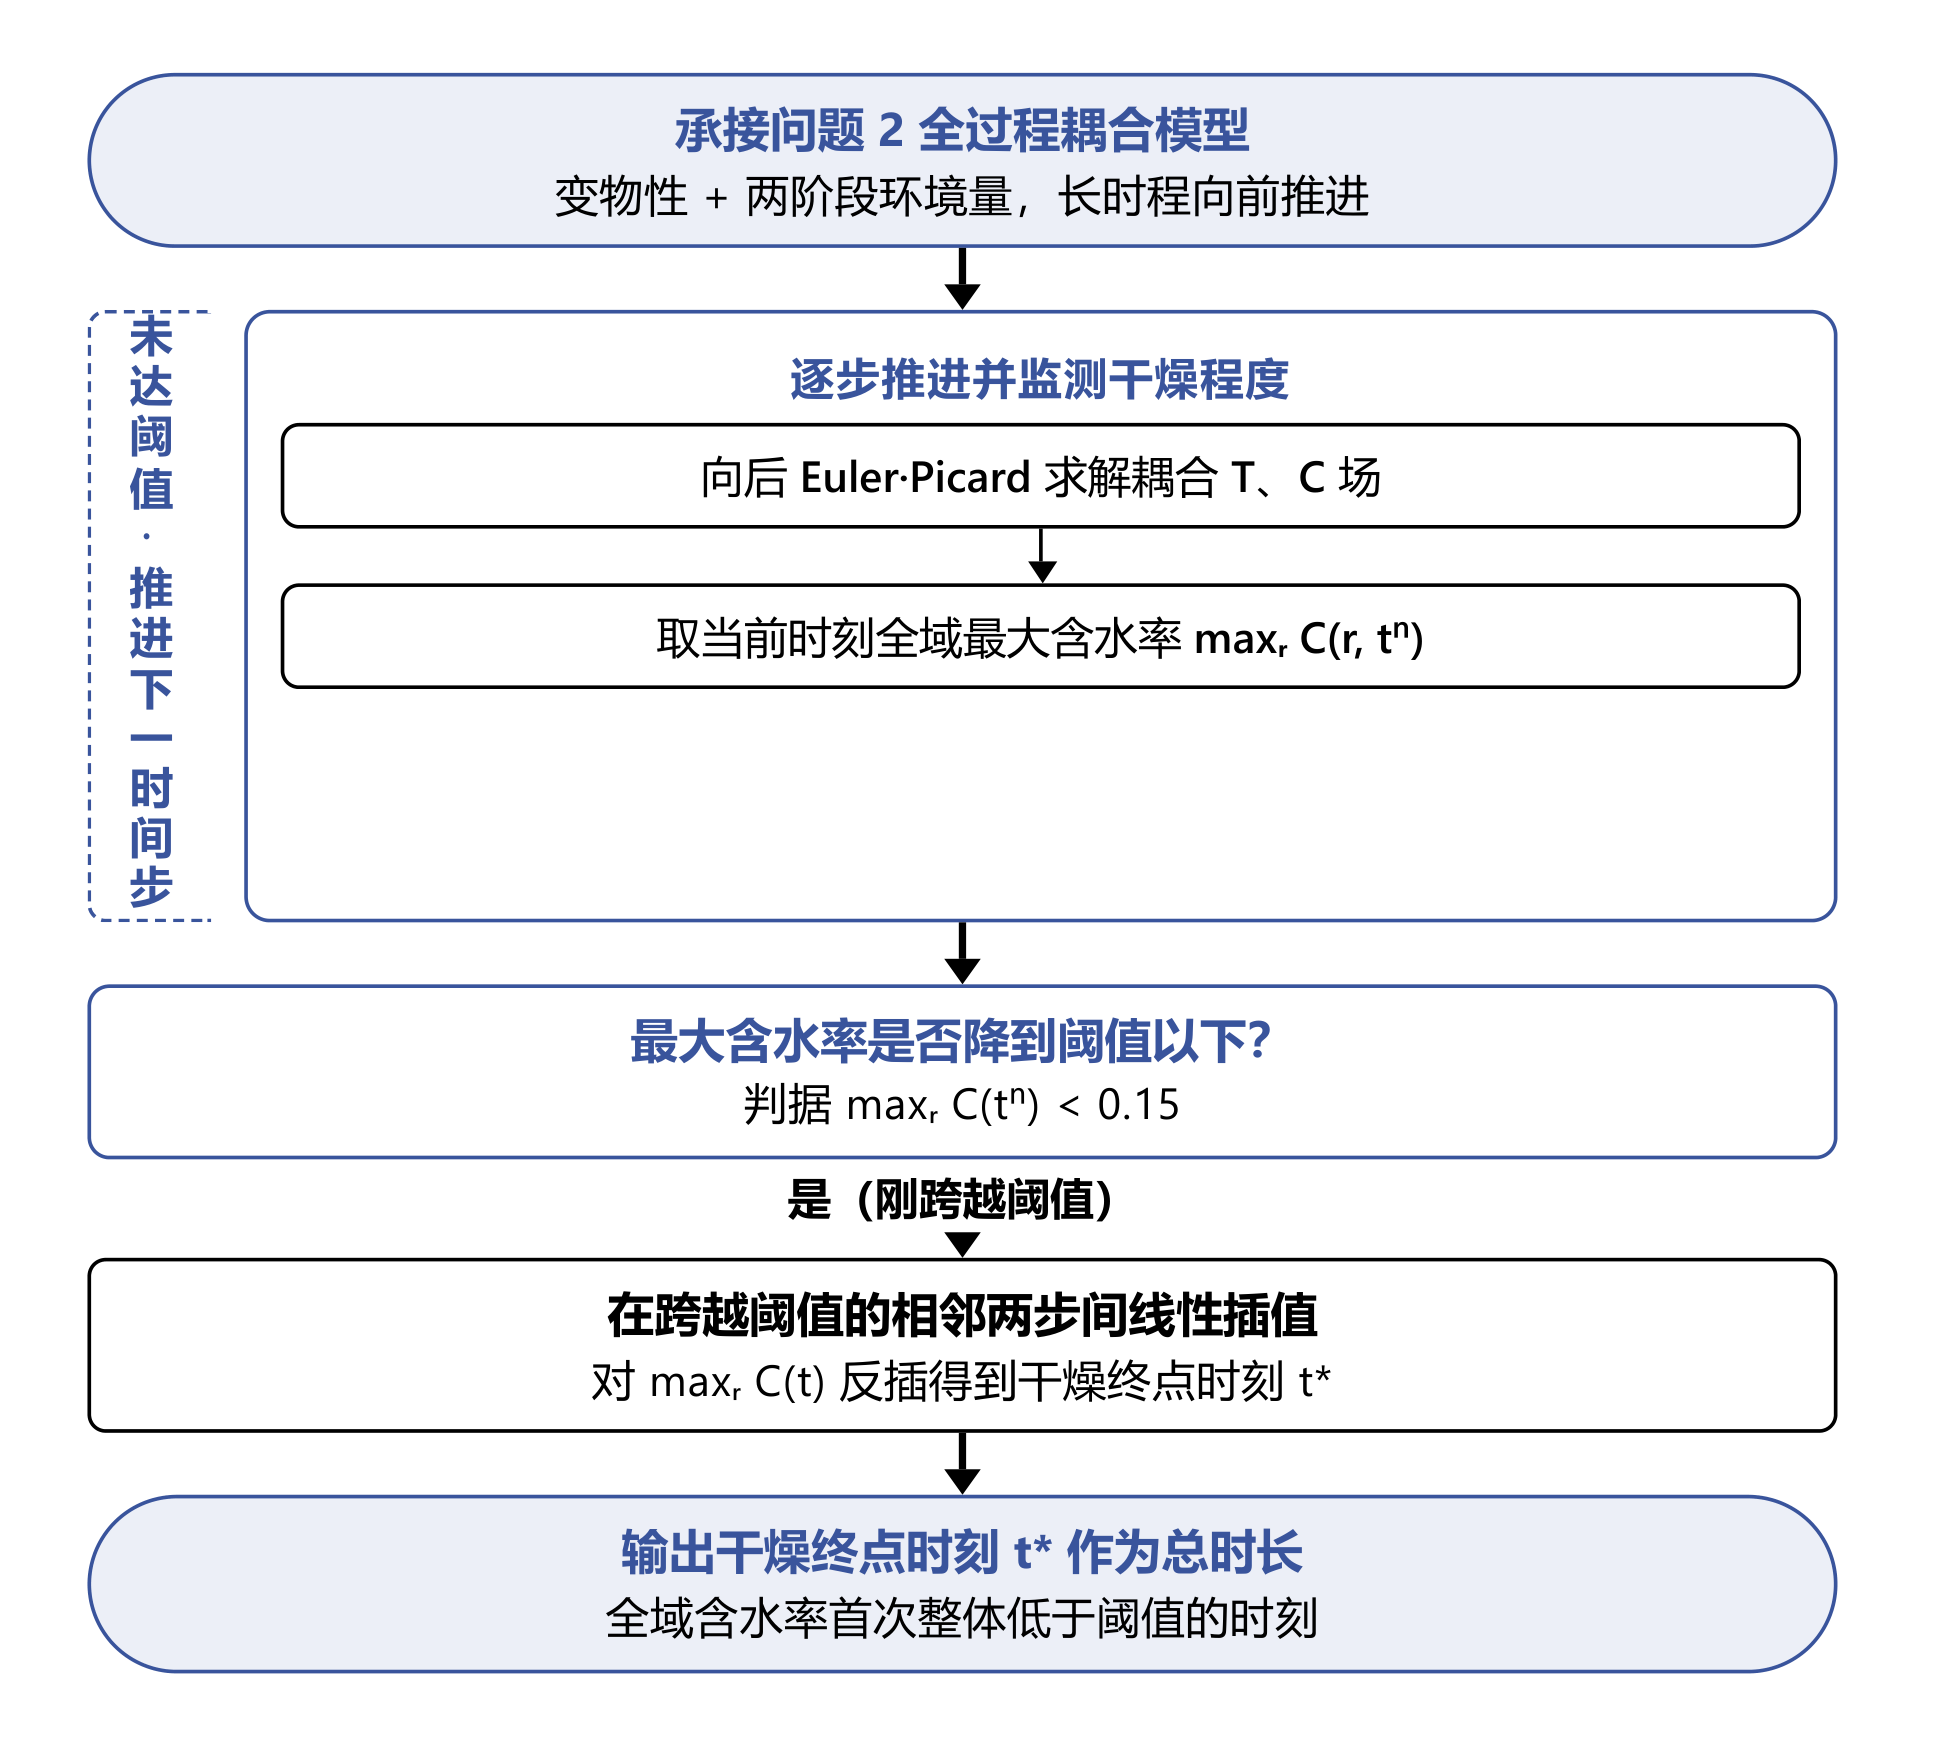
\includegraphics[width=0.9\textwidth,height=0.8\textheight,keepaspectratio]{figures/fig_flow_q3.pdf}
  \caption{问题 3 求解流程：阈值判定与插值定终点}
  \label{fig:flow_q3}
\end{figure}

\begin{figure}[H]
  \centering
  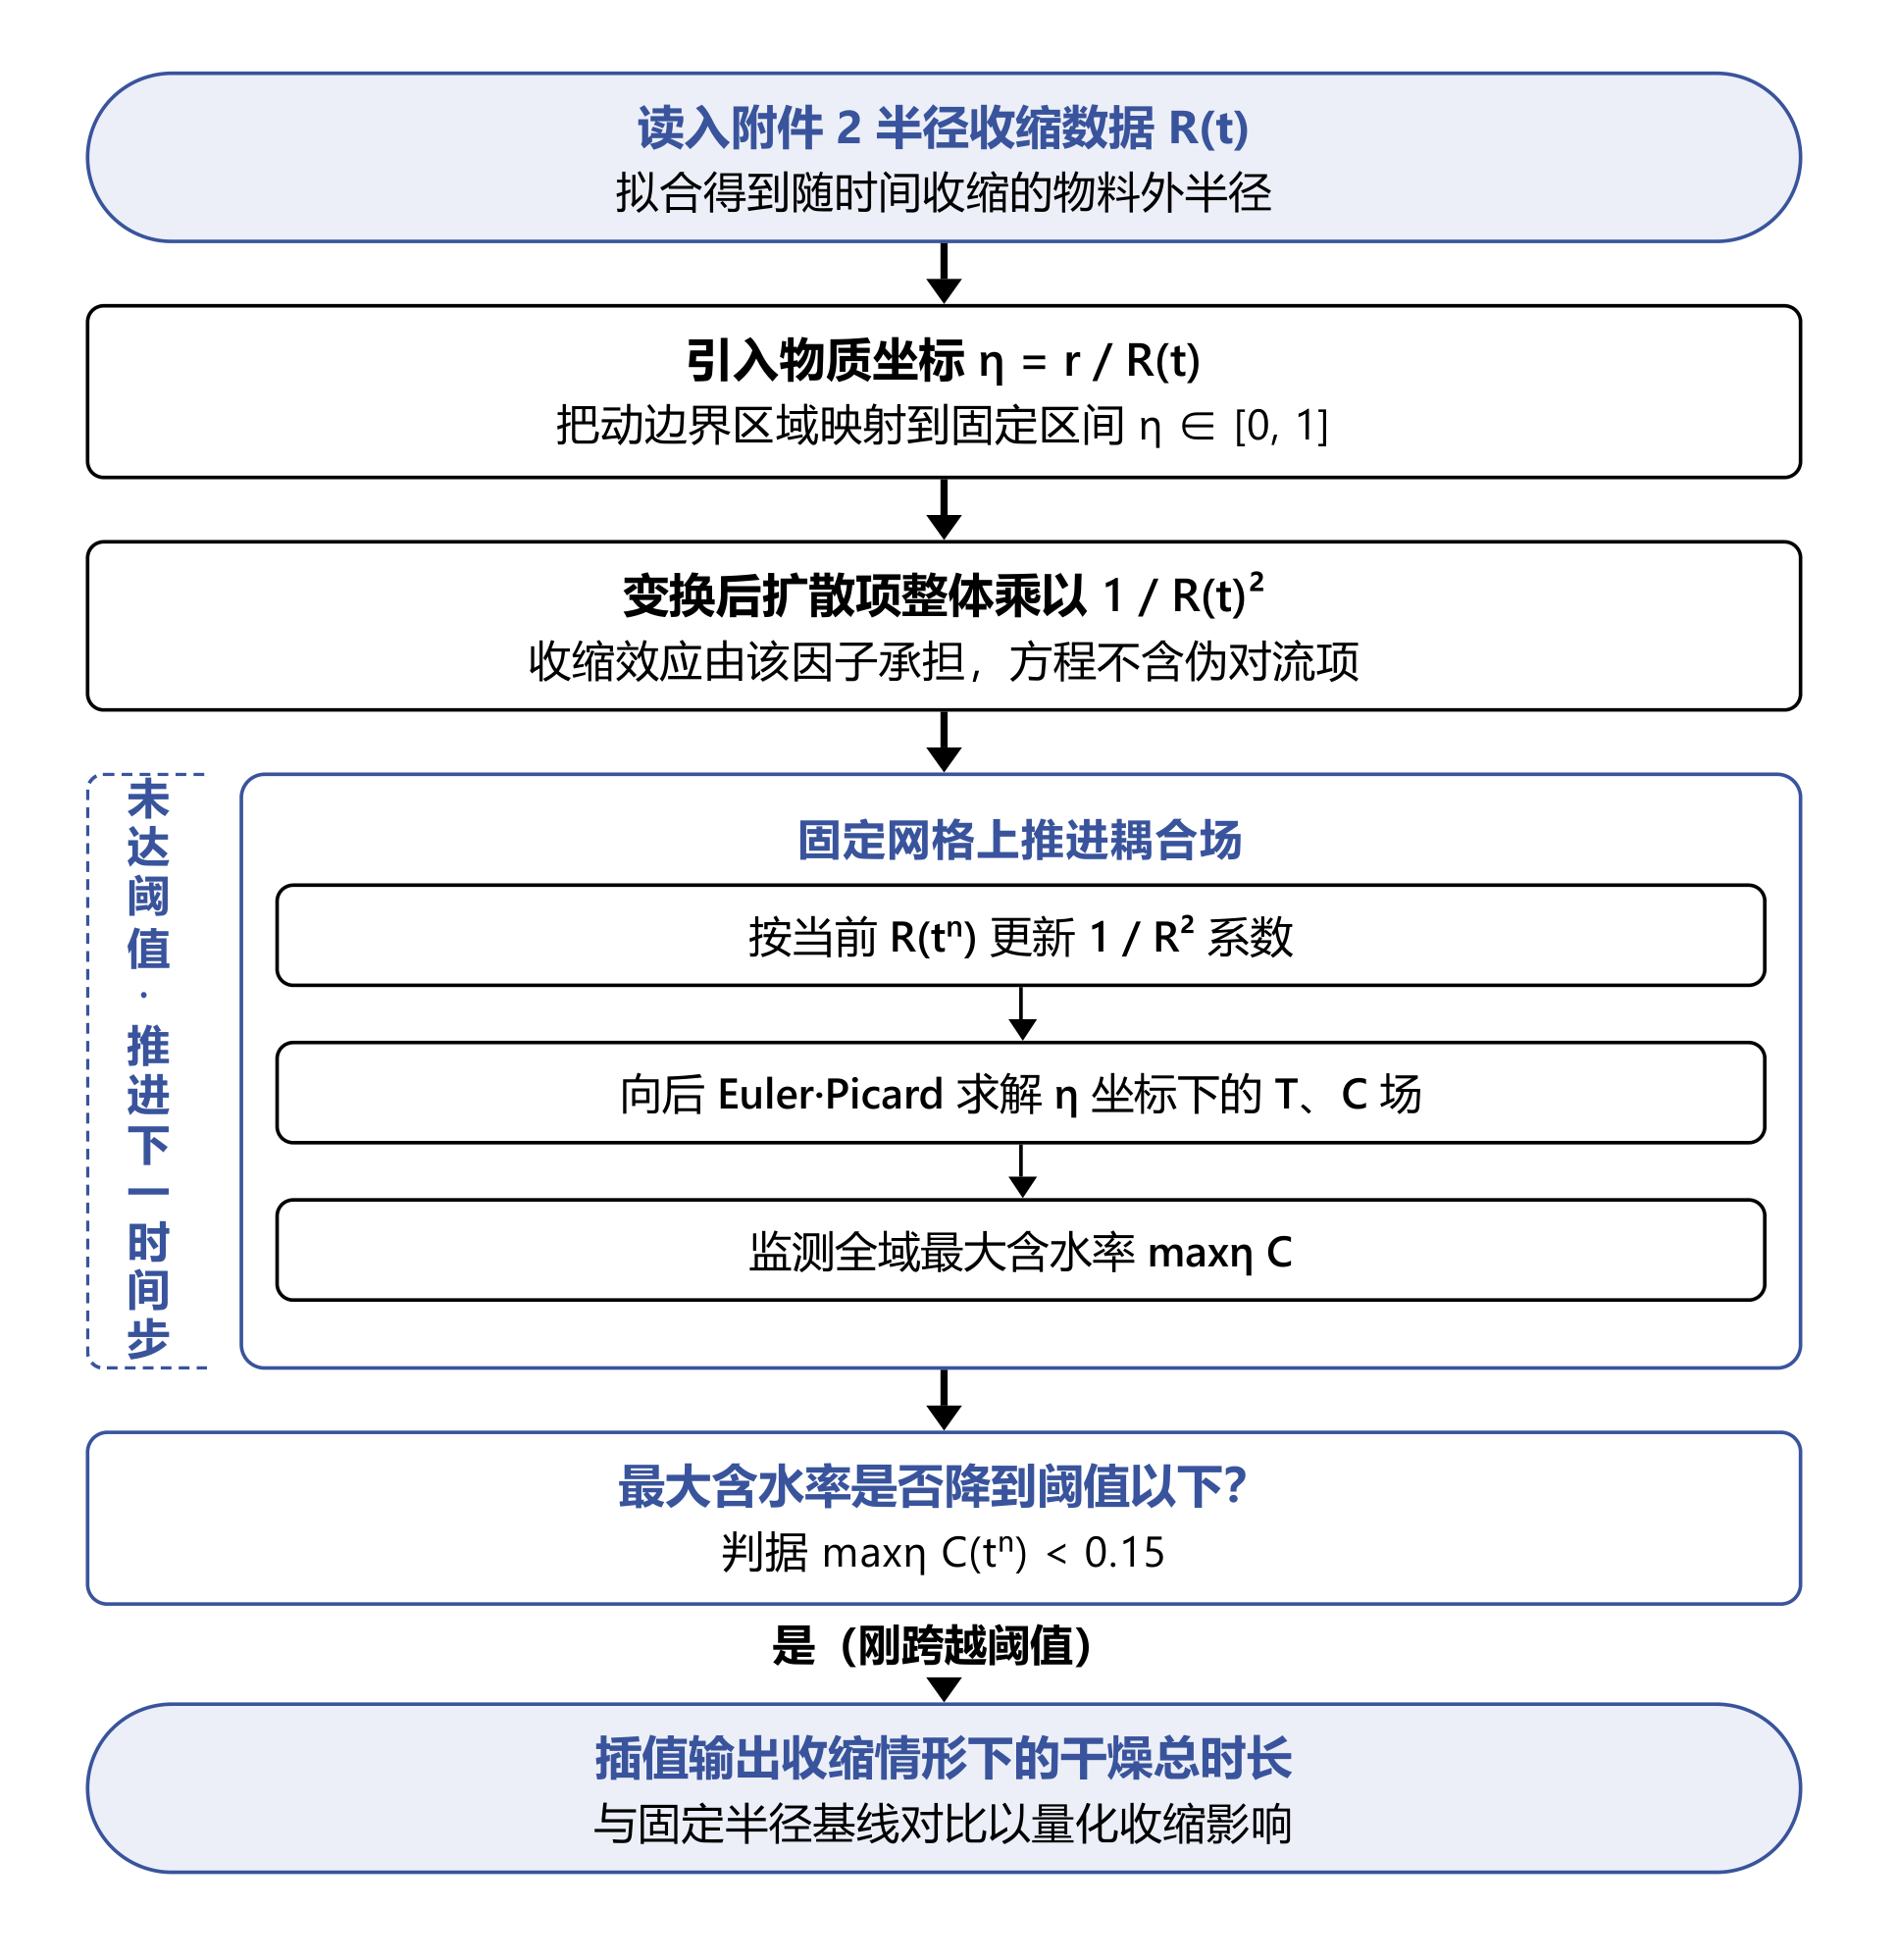
\includegraphics[width=0.9\textwidth,height=0.8\textheight,keepaspectratio]{figures/fig_flow_q4.pdf}
  \caption{问题 4 求解流程：物质坐标下的动边界推进}
  \label{fig:flow_q4}
\end{figure}

\begin{figure}[H]
  \centering
  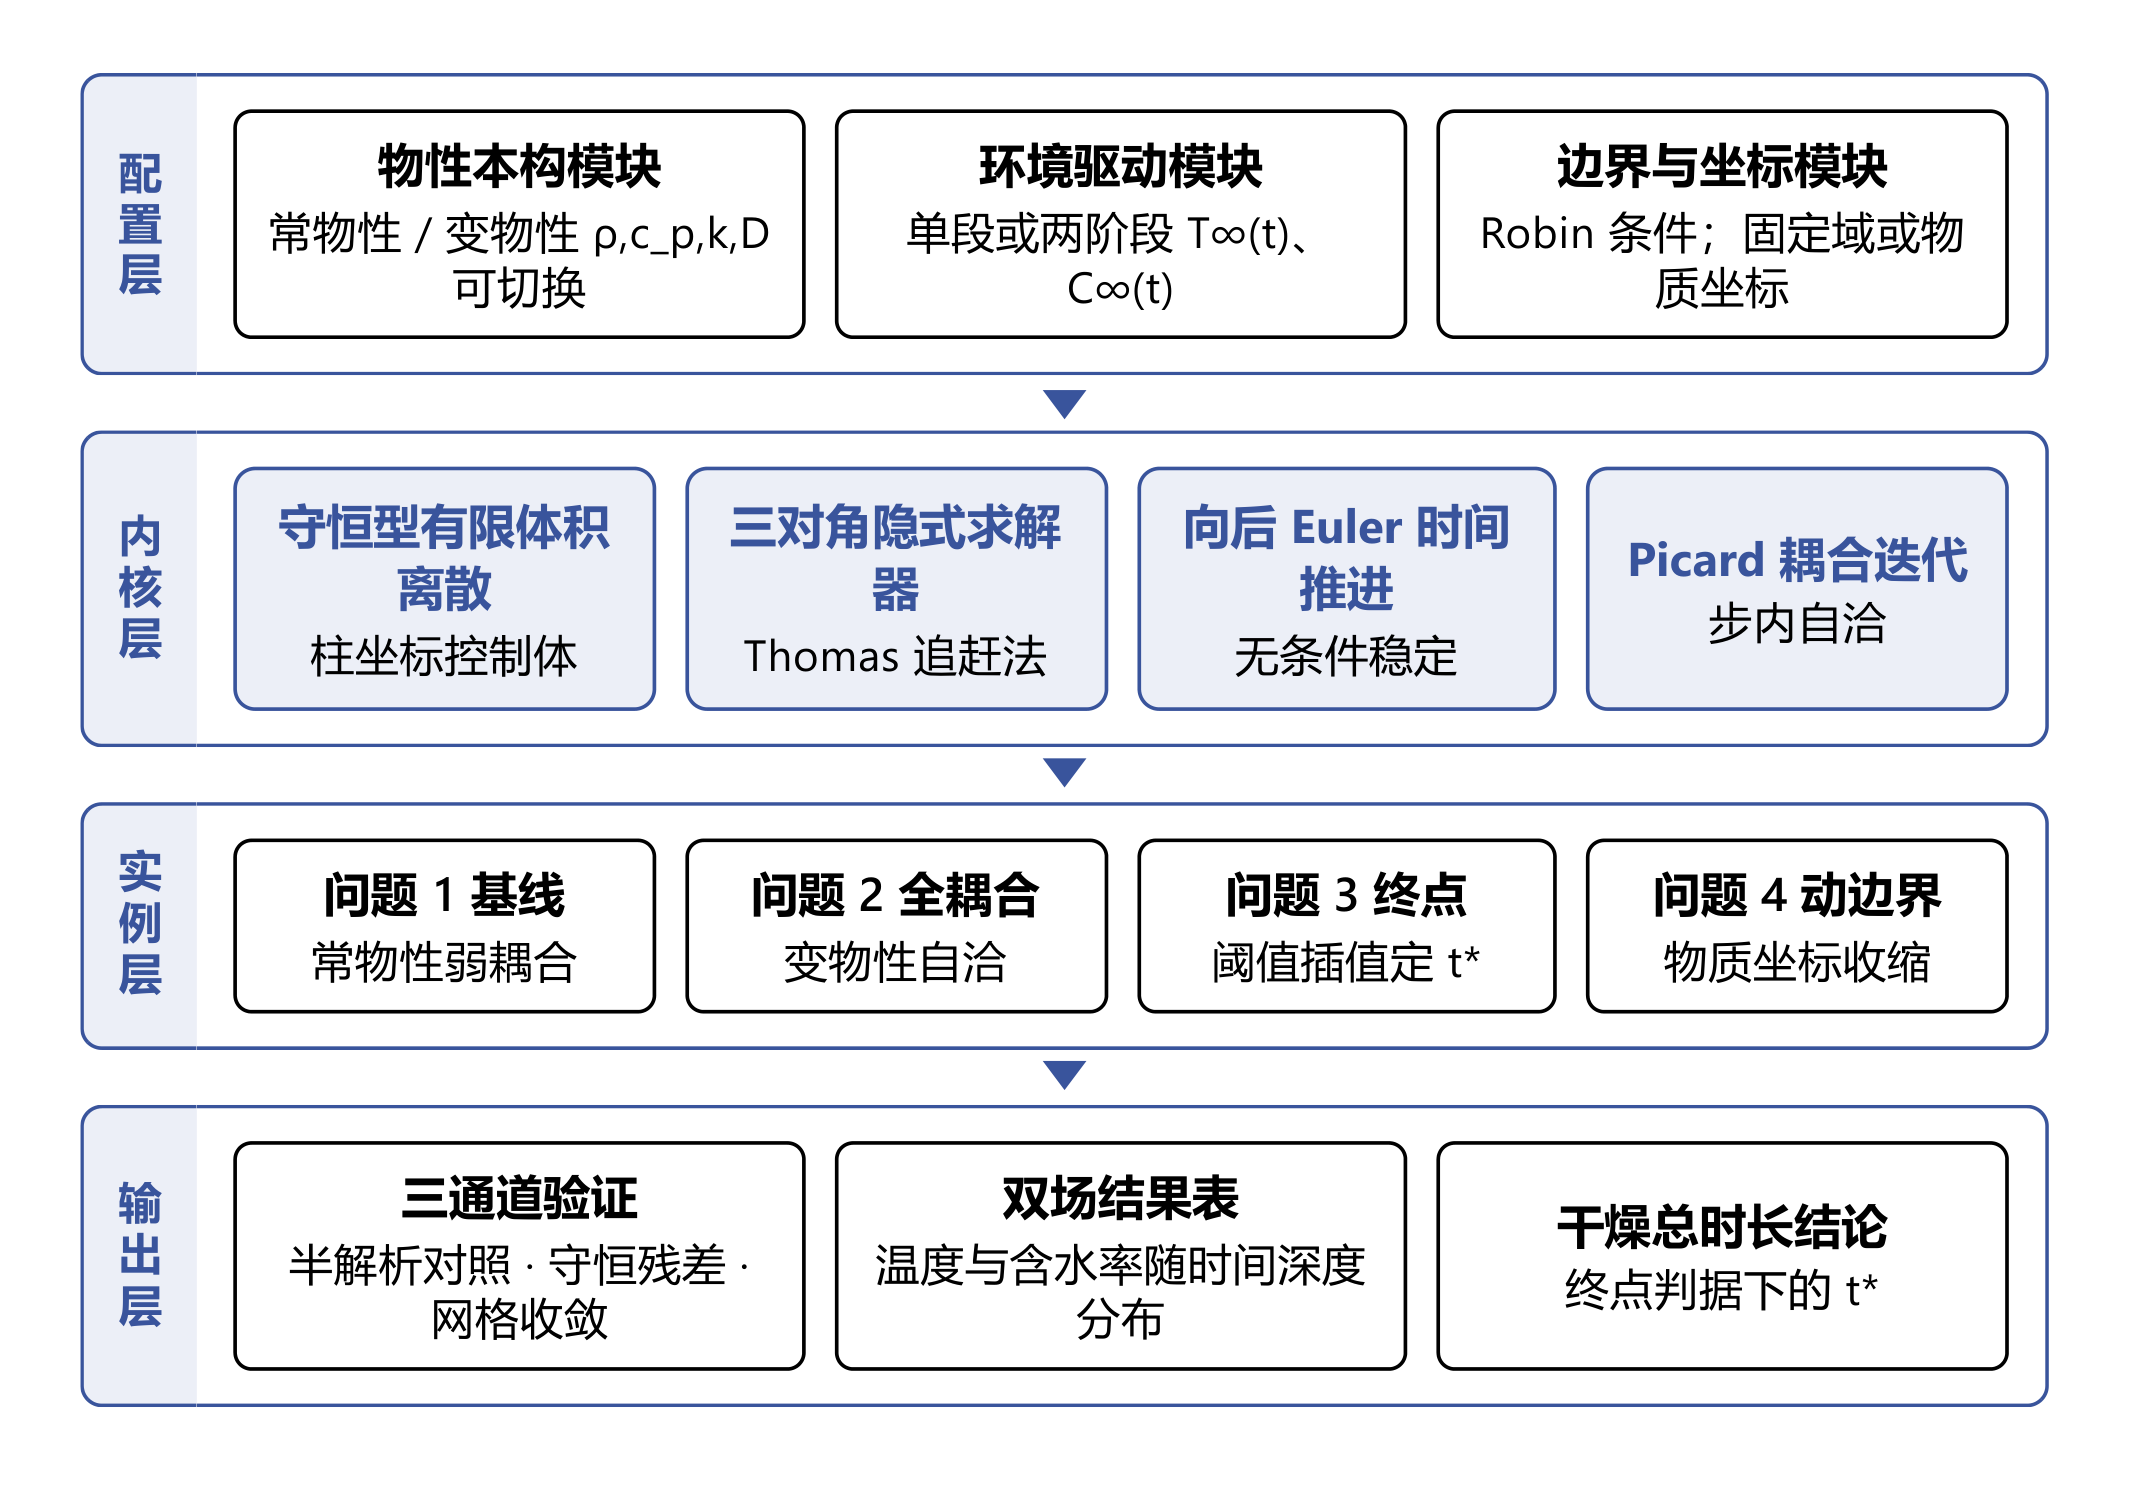
\includegraphics[width=0.9\textwidth,height=0.8\textheight,keepaspectratio]{figures/fig_solver_architecture.pdf}
  \caption{求解器架构：一套内核 + 四组配置}
  \label{fig:solver_architecture}
\end{figure}

% ── 几何与离散构造（TikZ 矢量图）──────────────────────────────
\begin{figure}[H]
  \centering
  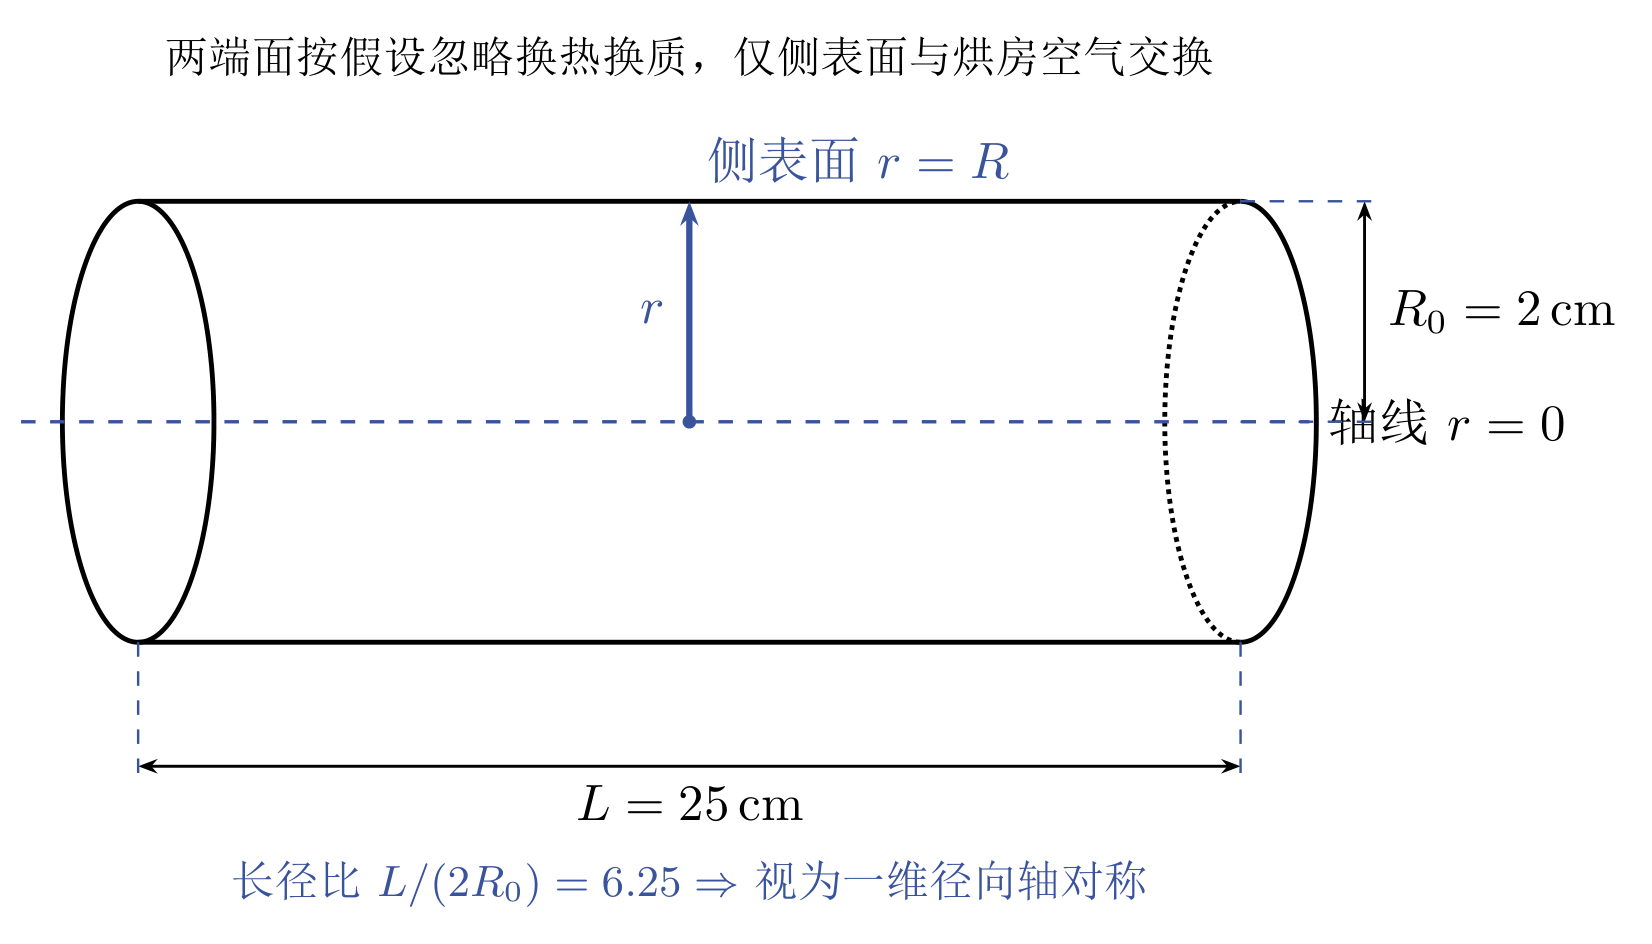
\includegraphics[width=0.9\textwidth,height=0.8\textheight,keepaspectratio]{figures/tikz_cylinder_geometry.pdf}
  \caption{圆柱几何、径向坐标与长径比}
  \label{fig:cylinder_geometry}
\end{figure}

\begin{figure}[H]
  \centering
  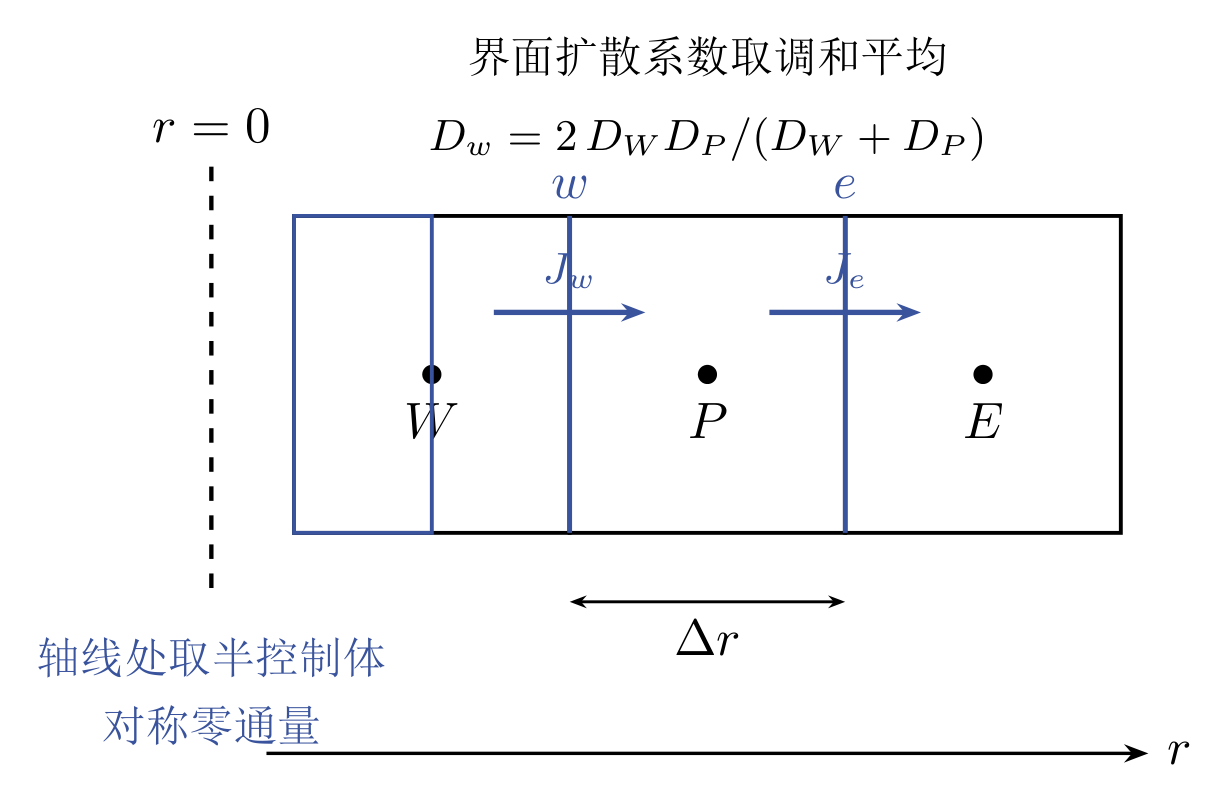
\includegraphics[width=0.9\textwidth,height=0.8\textheight,keepaspectratio]{figures/tikz_control_volume.pdf}
  \caption{守恒型有限体积径向控制体与界面通量}
  \label{fig:control_volume}
\end{figure}

\begin{figure}[H]
  \centering
  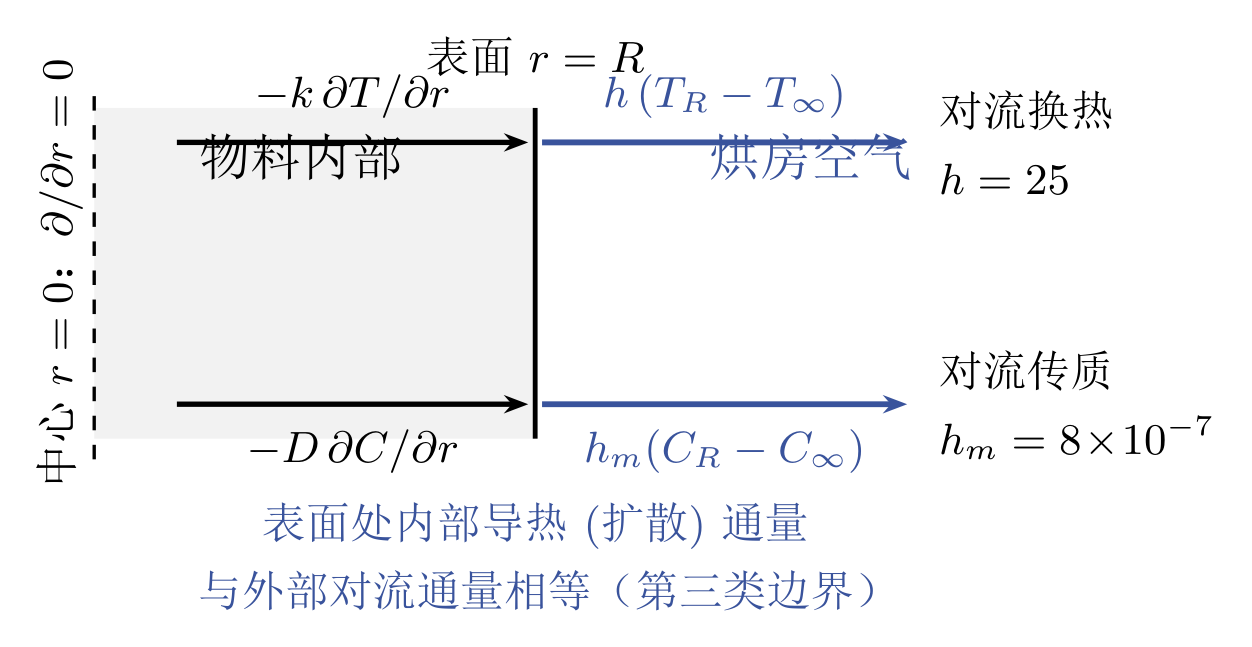
\includegraphics[width=0.9\textwidth,height=0.8\textheight,keepaspectratio]{figures/tikz_boundary_conditions.pdf}
  \caption{表面两个 Robin 条件的通量平衡}
  \label{fig:boundary_conditions}
\end{figure}

\begin{figure}[H]
  \centering
  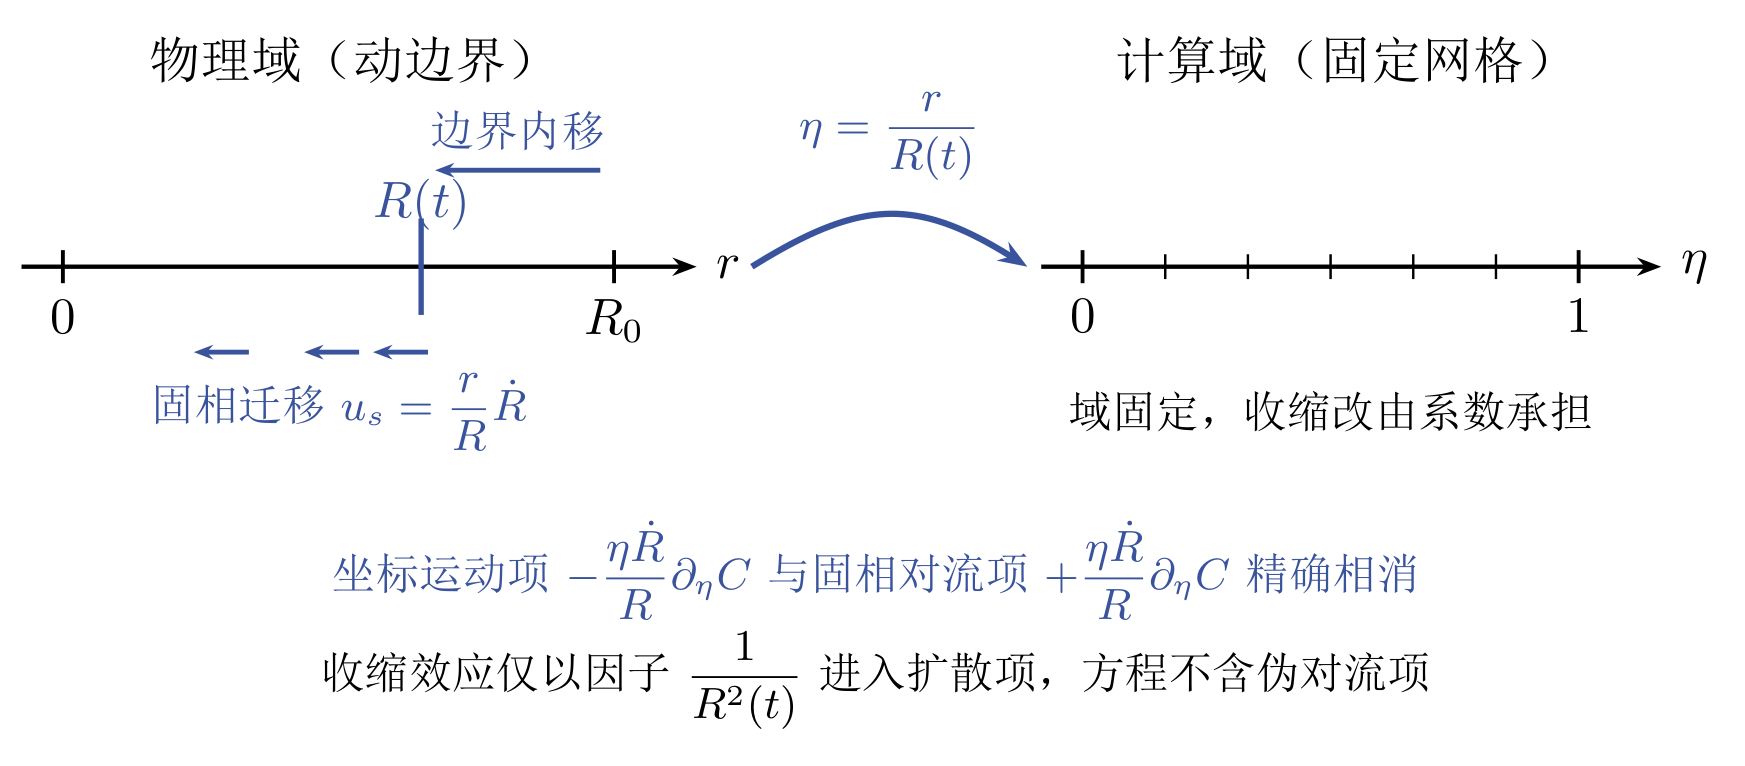
\includegraphics[width=0.9\textwidth,height=0.8\textheight,keepaspectratio]{figures/tikz_moving_boundary_transform.pdf}
  \caption{物质坐标变换与伪对流项的相消}
  \label{fig:moving_boundary_transform}
\end{figure}
